\chapter{Sucre}
\section*{15 avril 2015}
A Potosi je quitte Lucie et Frédéric qui vont directement vers La Paz. \newline
 De mon côté je continue vers Sucre : 150km avec beaucoup de descente pour passer de 4000m à 2800m \newline
 \newline
\centerline{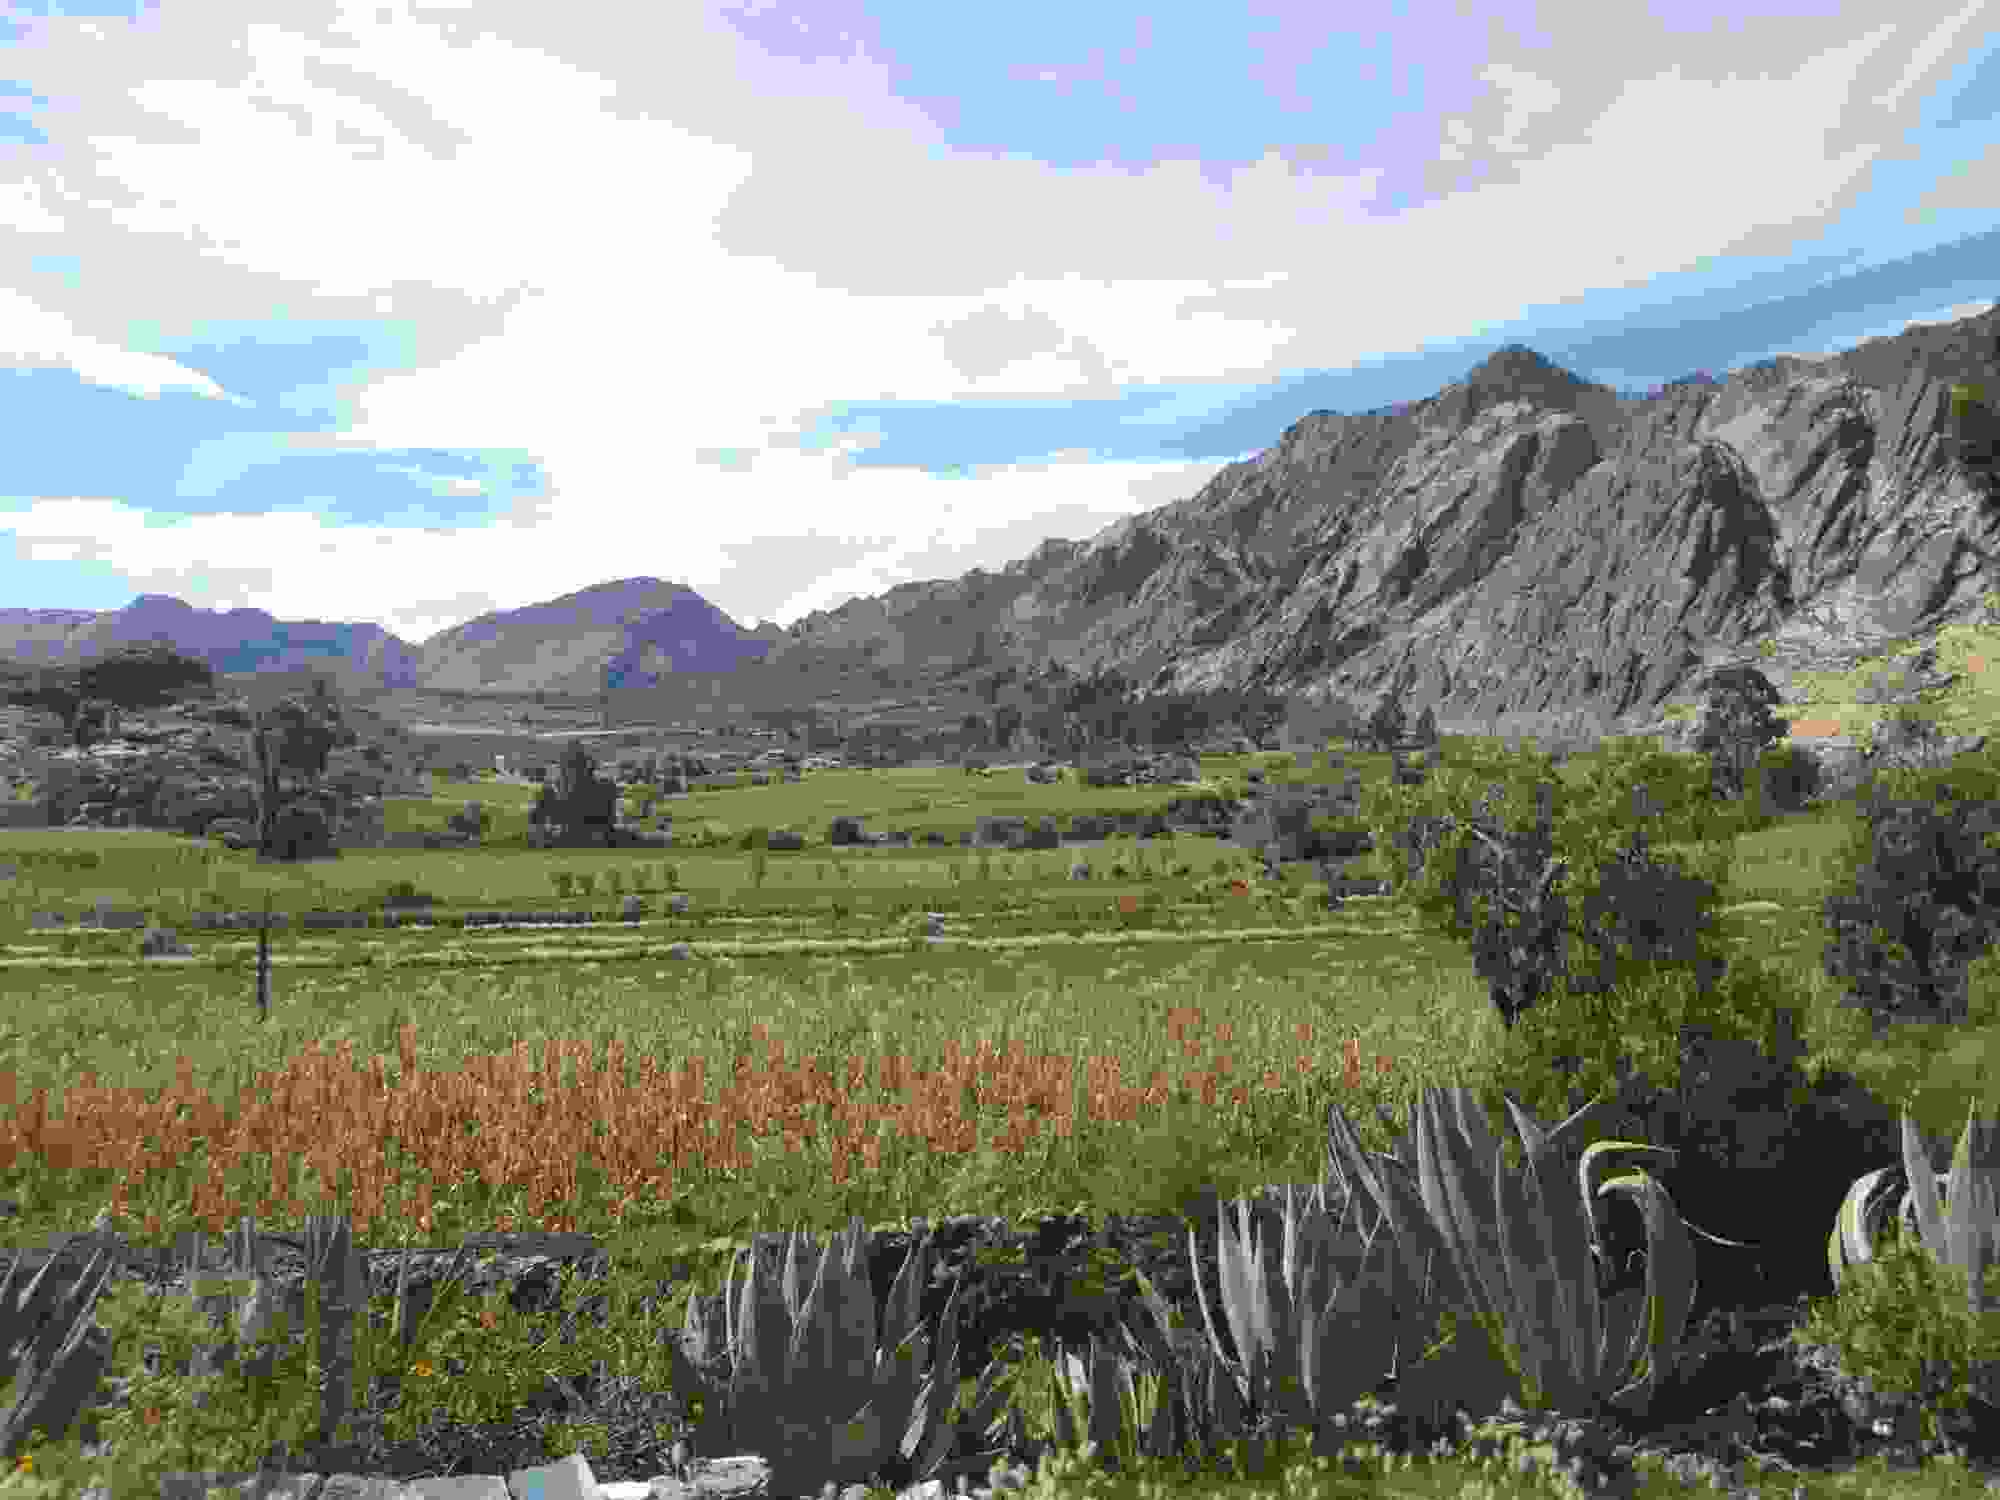
\includegraphics[width=\mywidth]{../wp-content/uploads/2015/04/wpid-wp-1429062375616.jpg} } 
 \newline
 \newline
\centerline{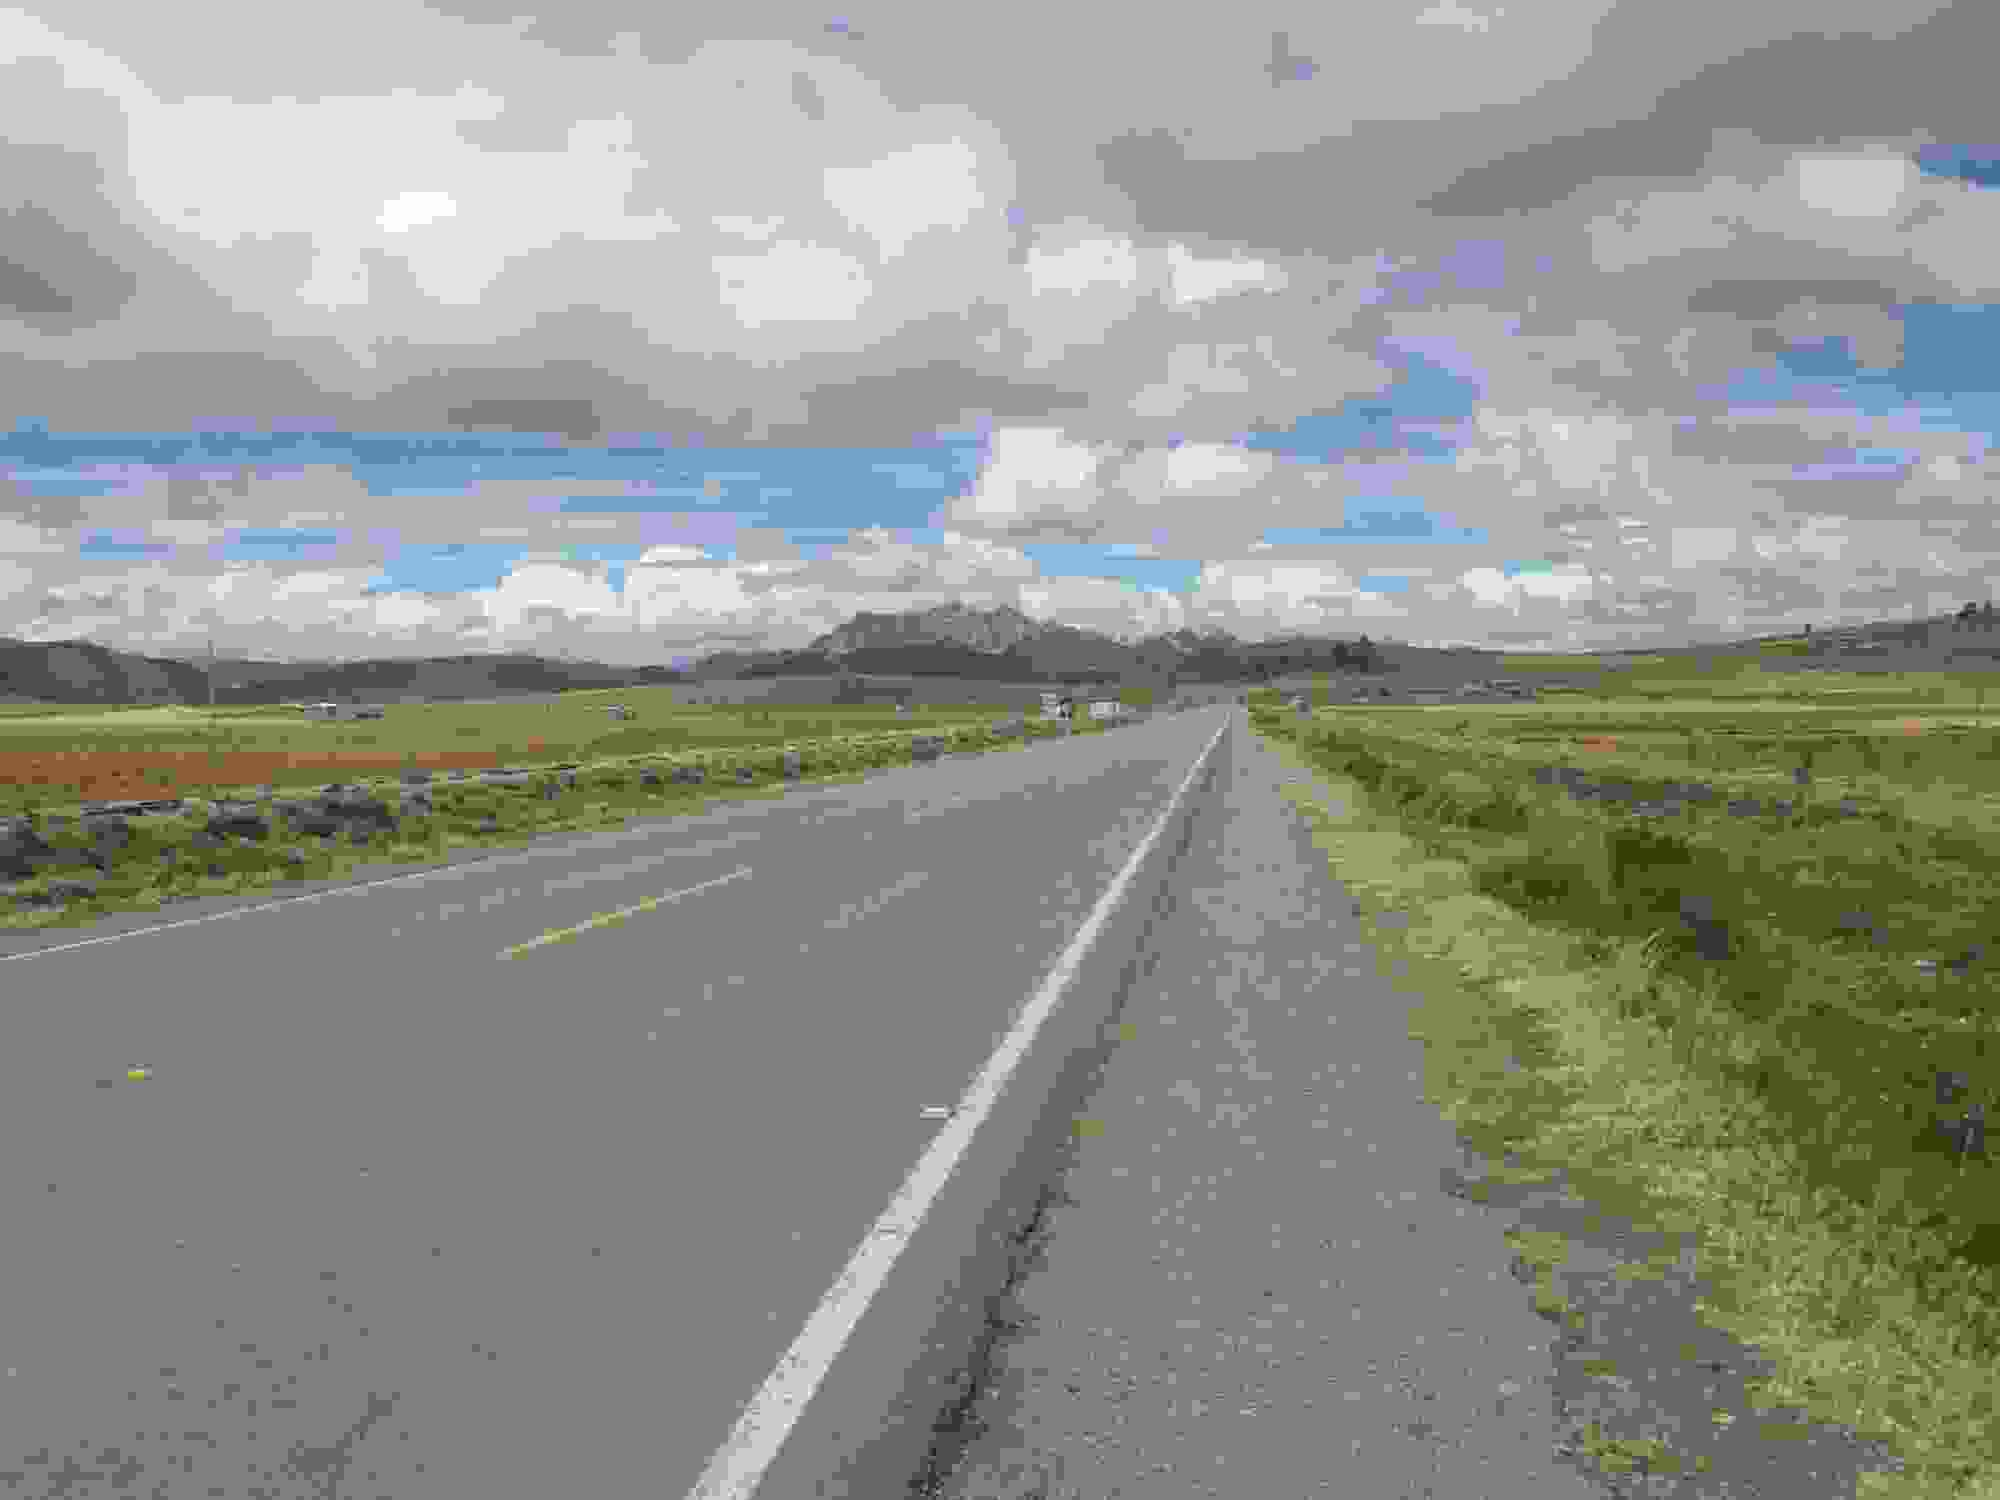
\includegraphics[width=\mywidth]{../wp-content/uploads/2015/04/wpid-wp-1429062400183.jpg} } 
 \newline
 Les lamas sont progressivement remplacés par les vaches et les moutons. Beaucoup de chiens aussi dont quelques uns un peu agressifs. \newline
 Toujours de beaux paysages sur la route.  \newline
 \newline
\centerline{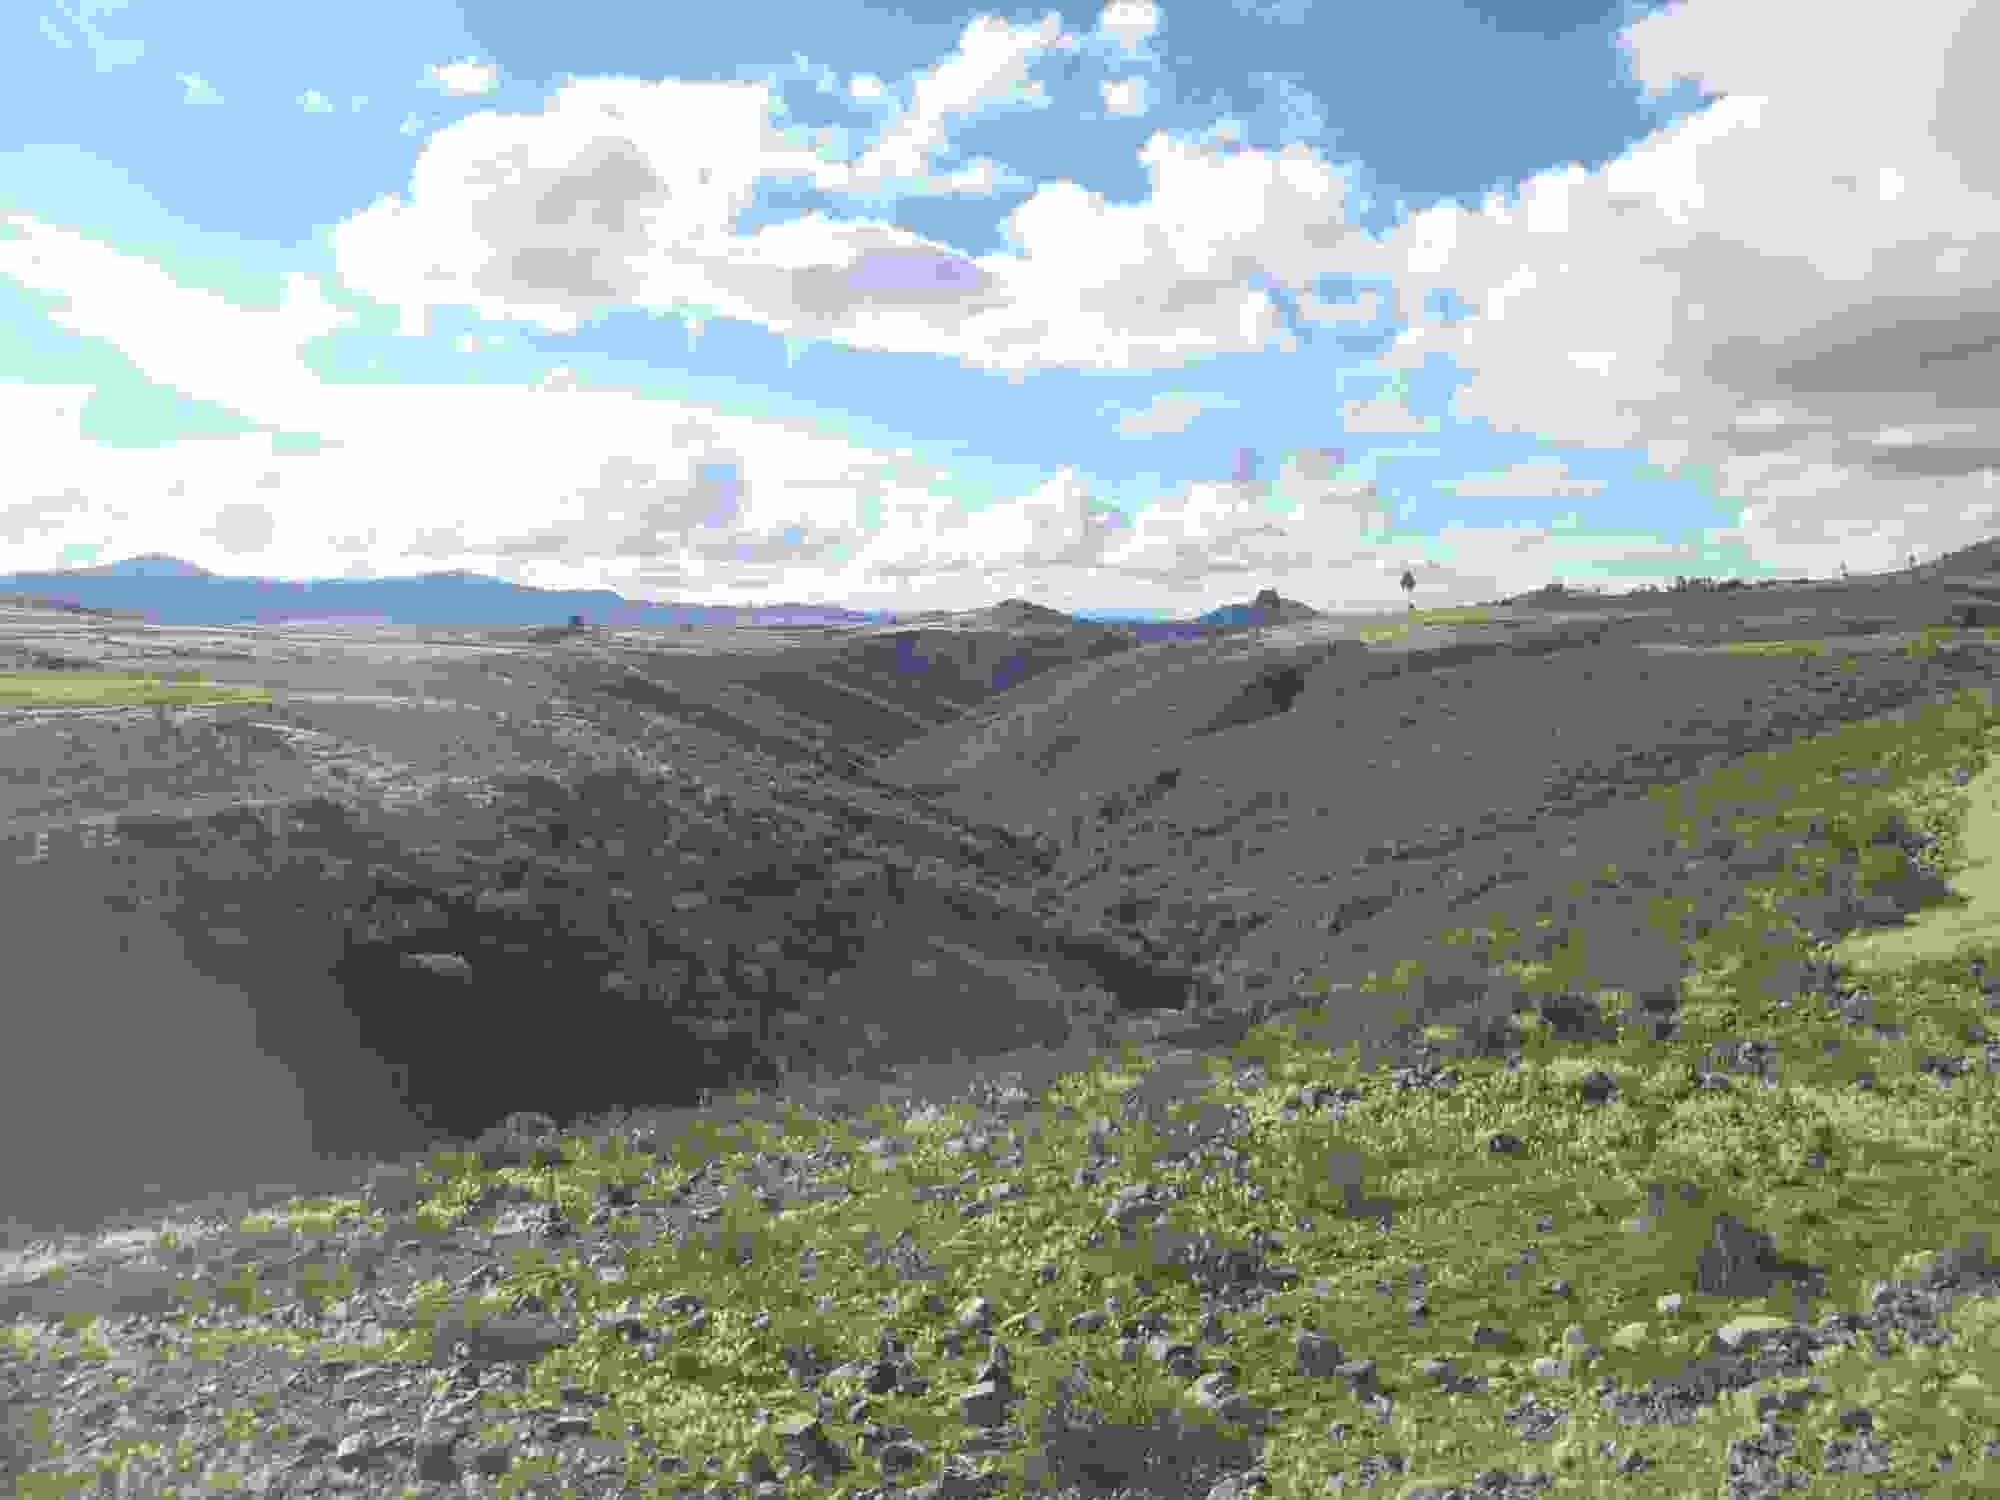
\includegraphics[width=\mywidth]{../wp-content/uploads/2015/04/wpid-wp-1429062516923.jpg} } 
 \newline
 \newline
\centerline{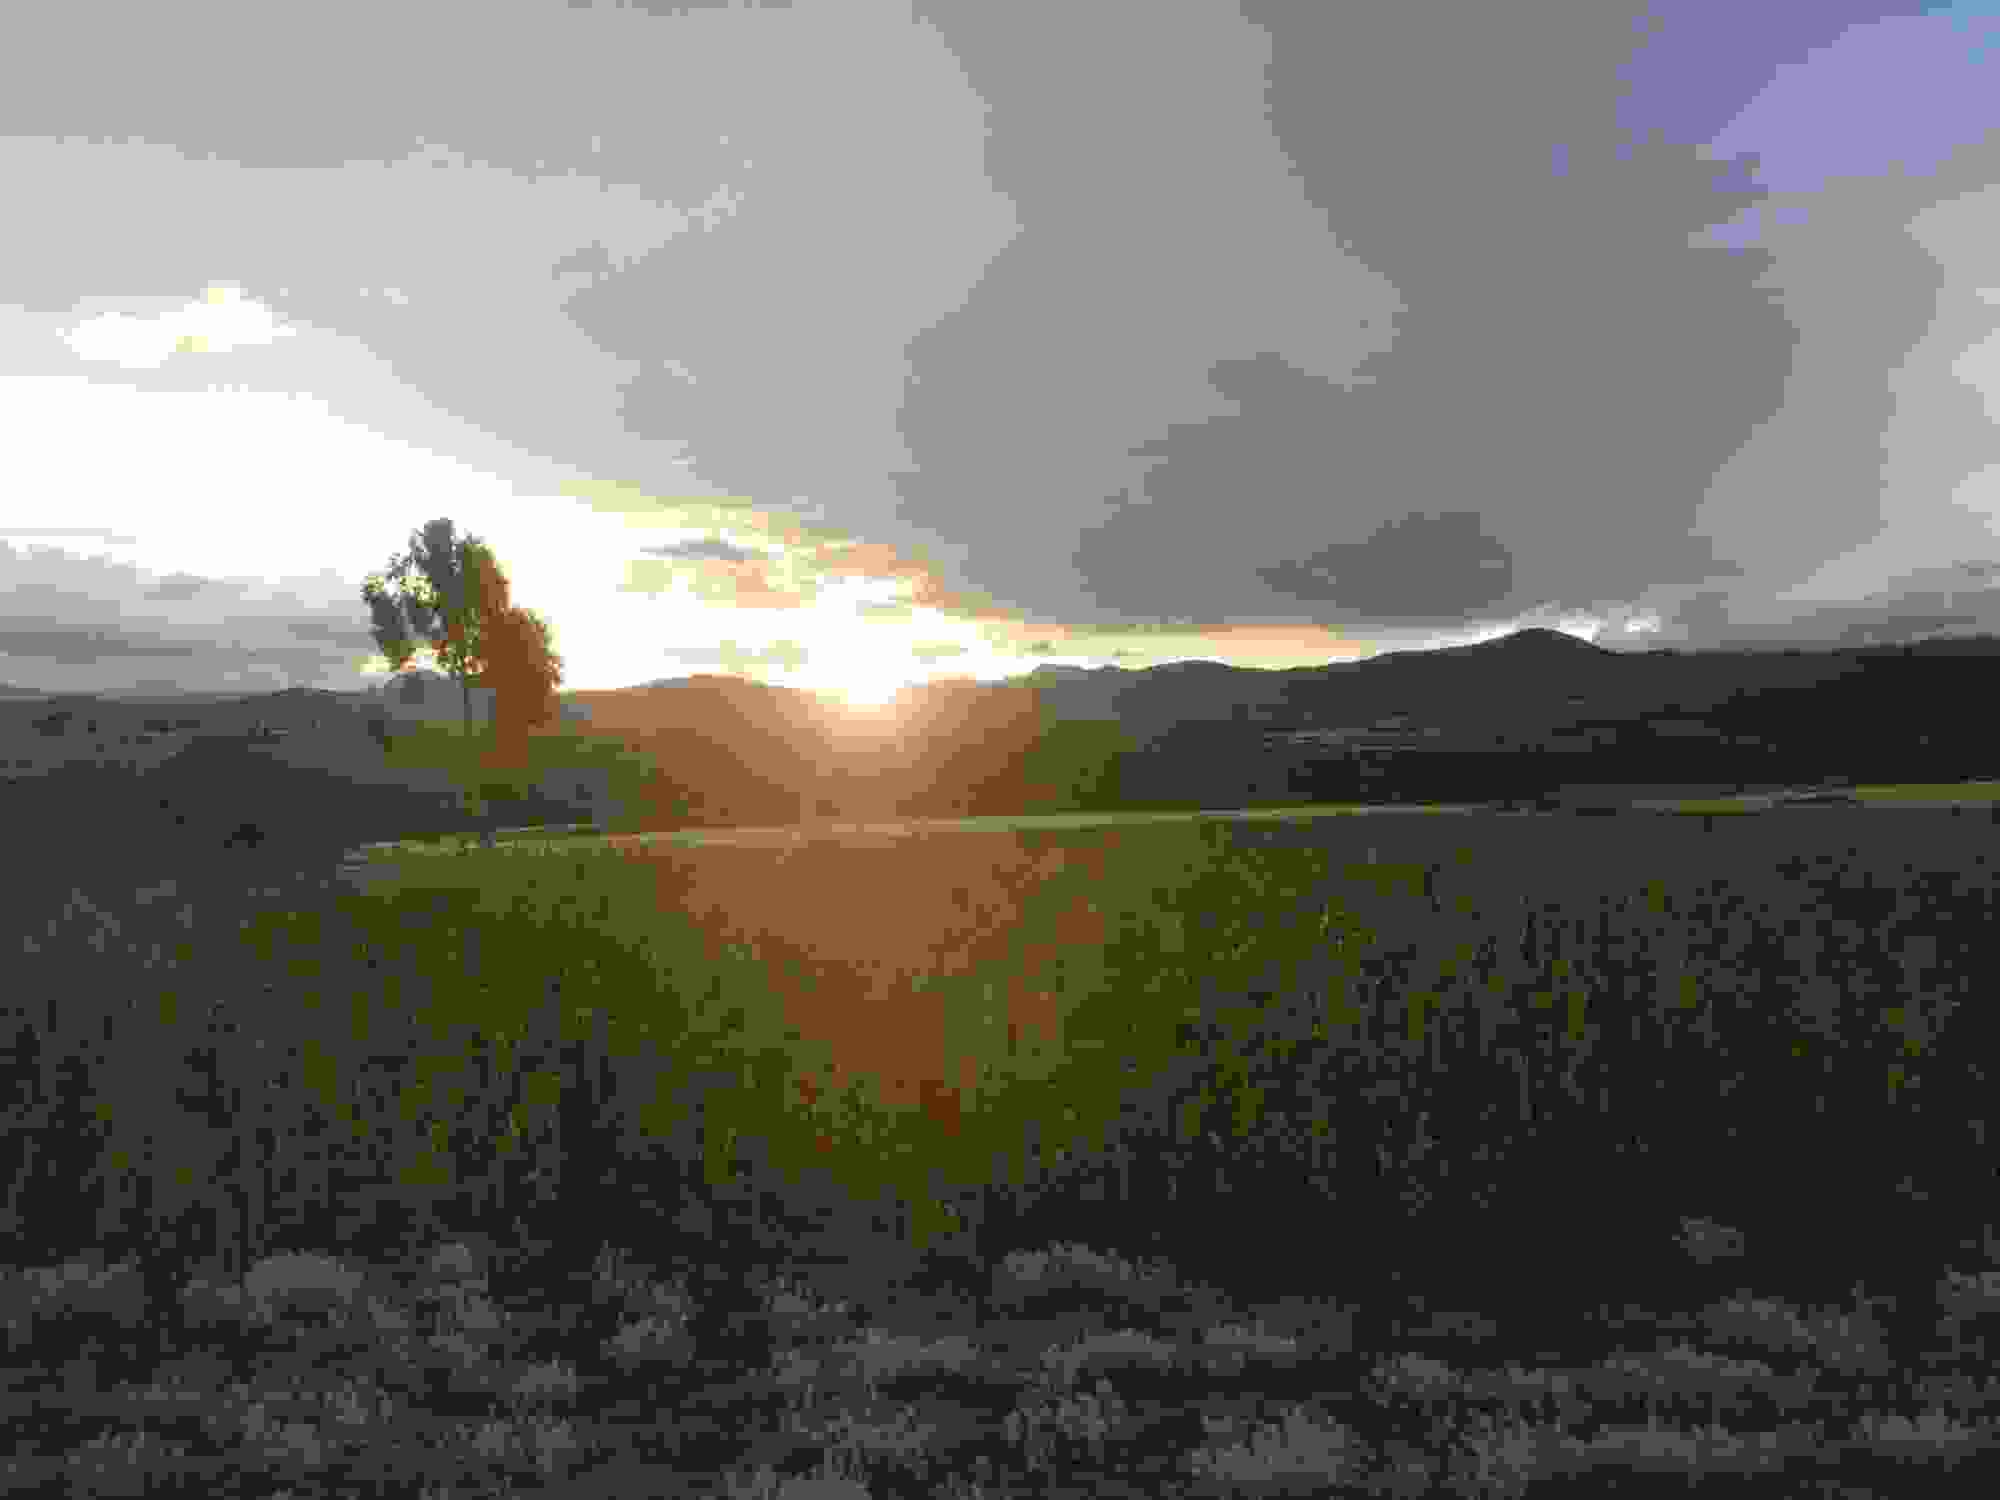
\includegraphics[width=\mywidth]{../wp-content/uploads/2015/04/wpid-wp-1429062575398.jpg} } 
 \newline
 \newline
\centerline{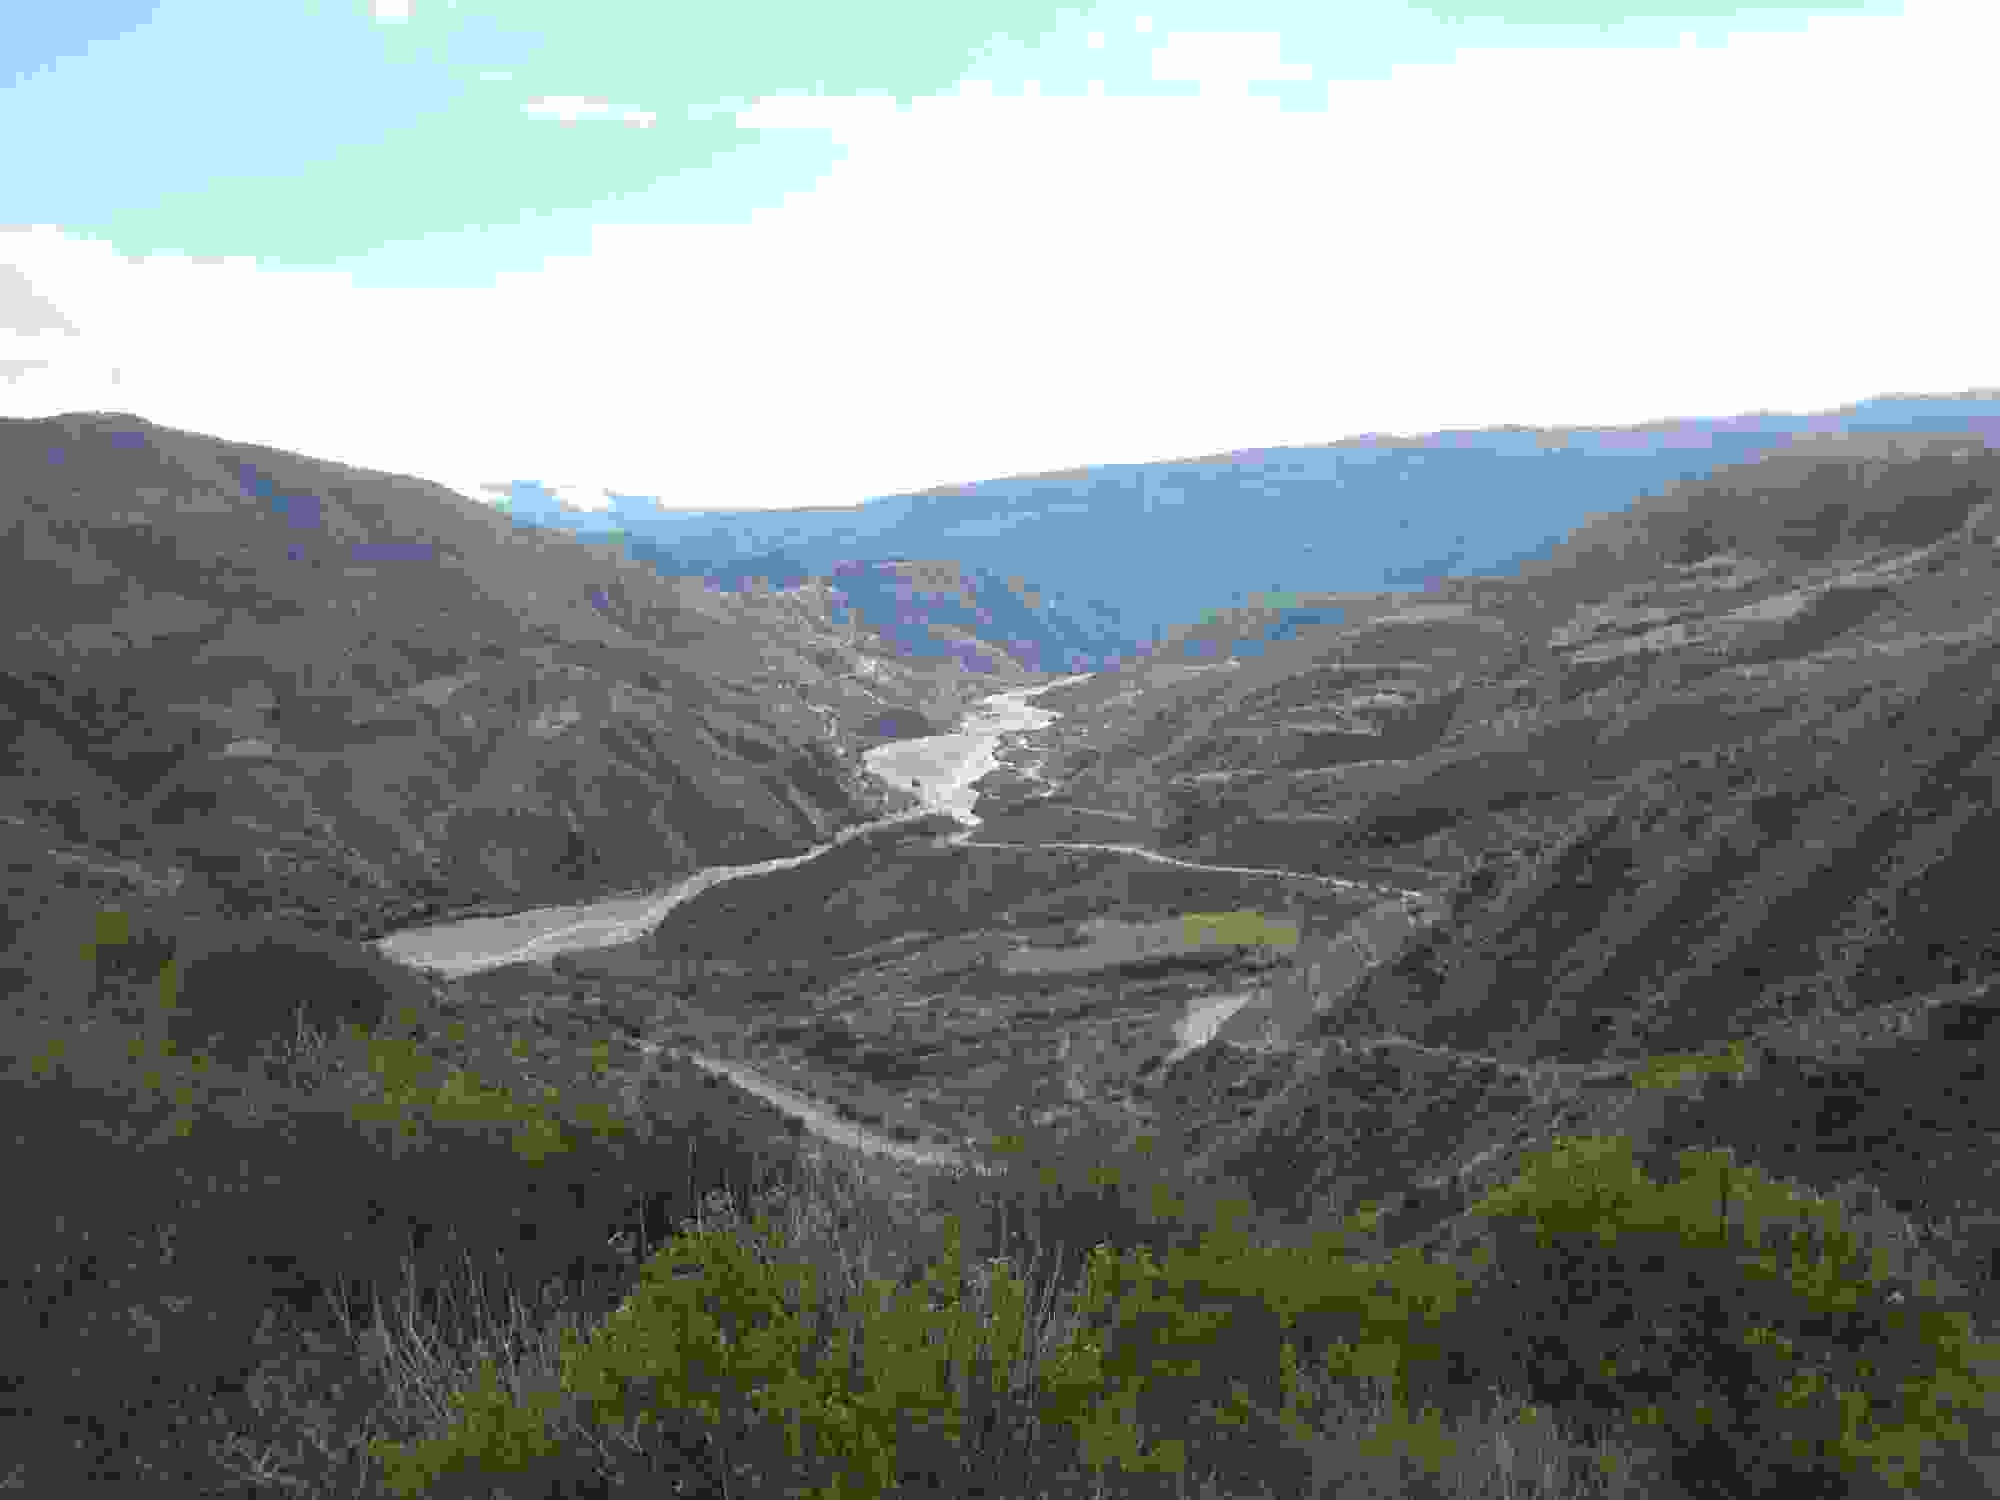
\includegraphics[width=\mywidth]{../wp-content/uploads/2015/04/wpid-wp-1429062588750.jpg} } 
 \newline
 En 2 jours j'arrive à Sucre, la capitale judiciaire du pays. \newline
 La ville contraste énormément avec ce que j'ai vu de la Bolivie jusqu'à présent : très agréable, plutôt propre et avec un climat doux. Même les gens semblent plus souriants.  \newline
 \newline
\centerline{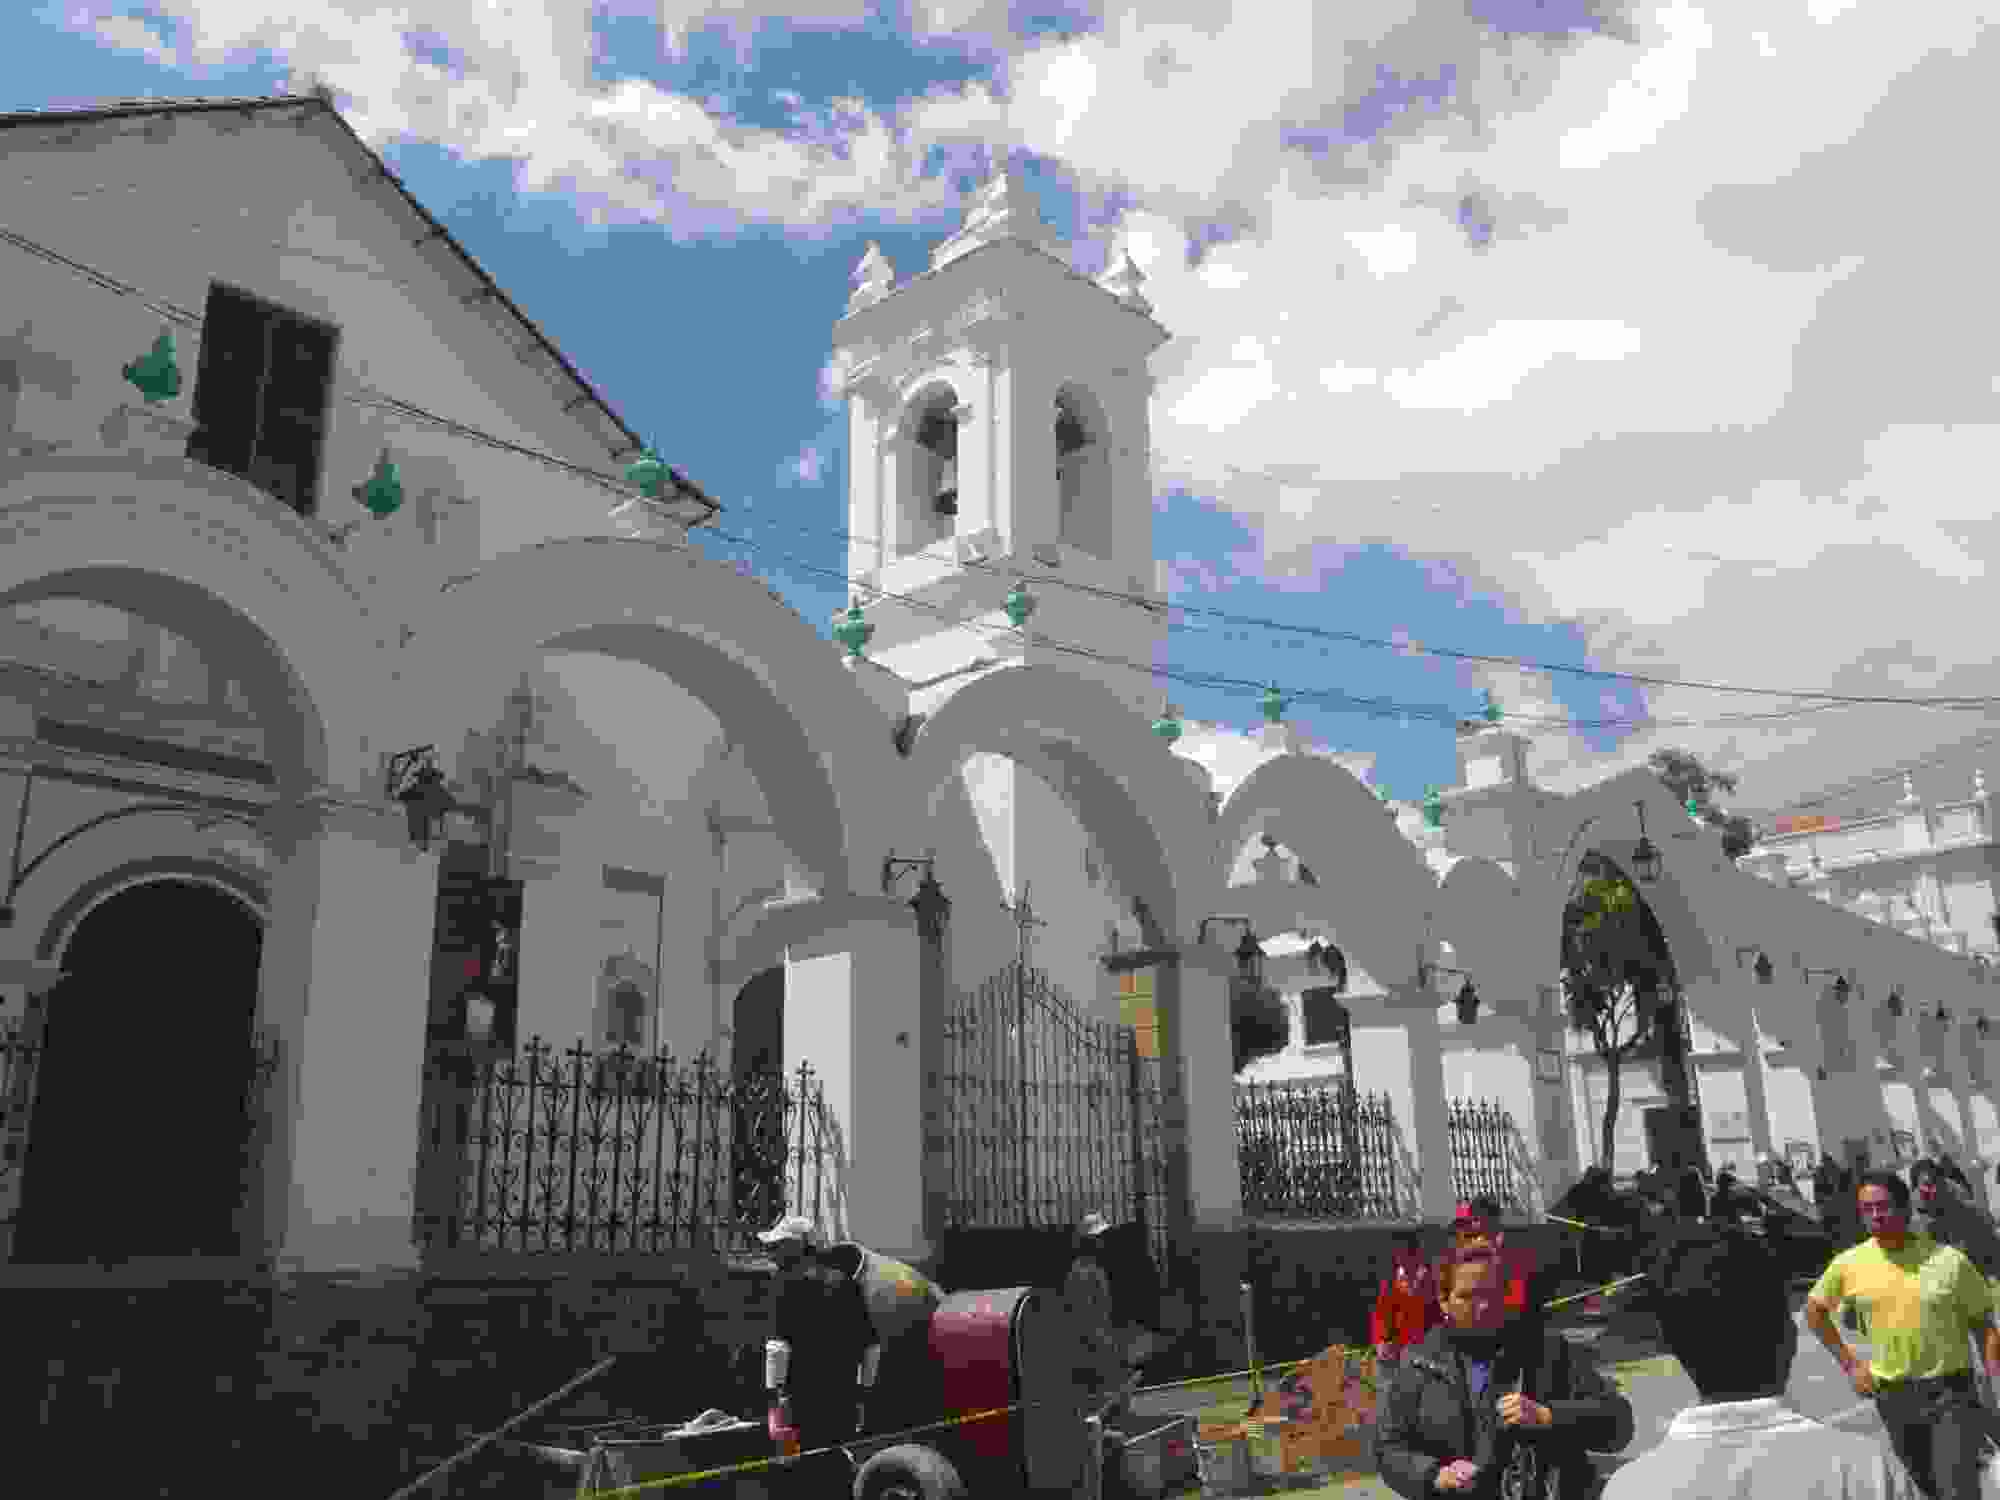
\includegraphics[width=\mywidth]{../wp-content/uploads/2015/04/wpid-wp-1429063237665.jpg} } 
 \newline
 \newline
\centerline{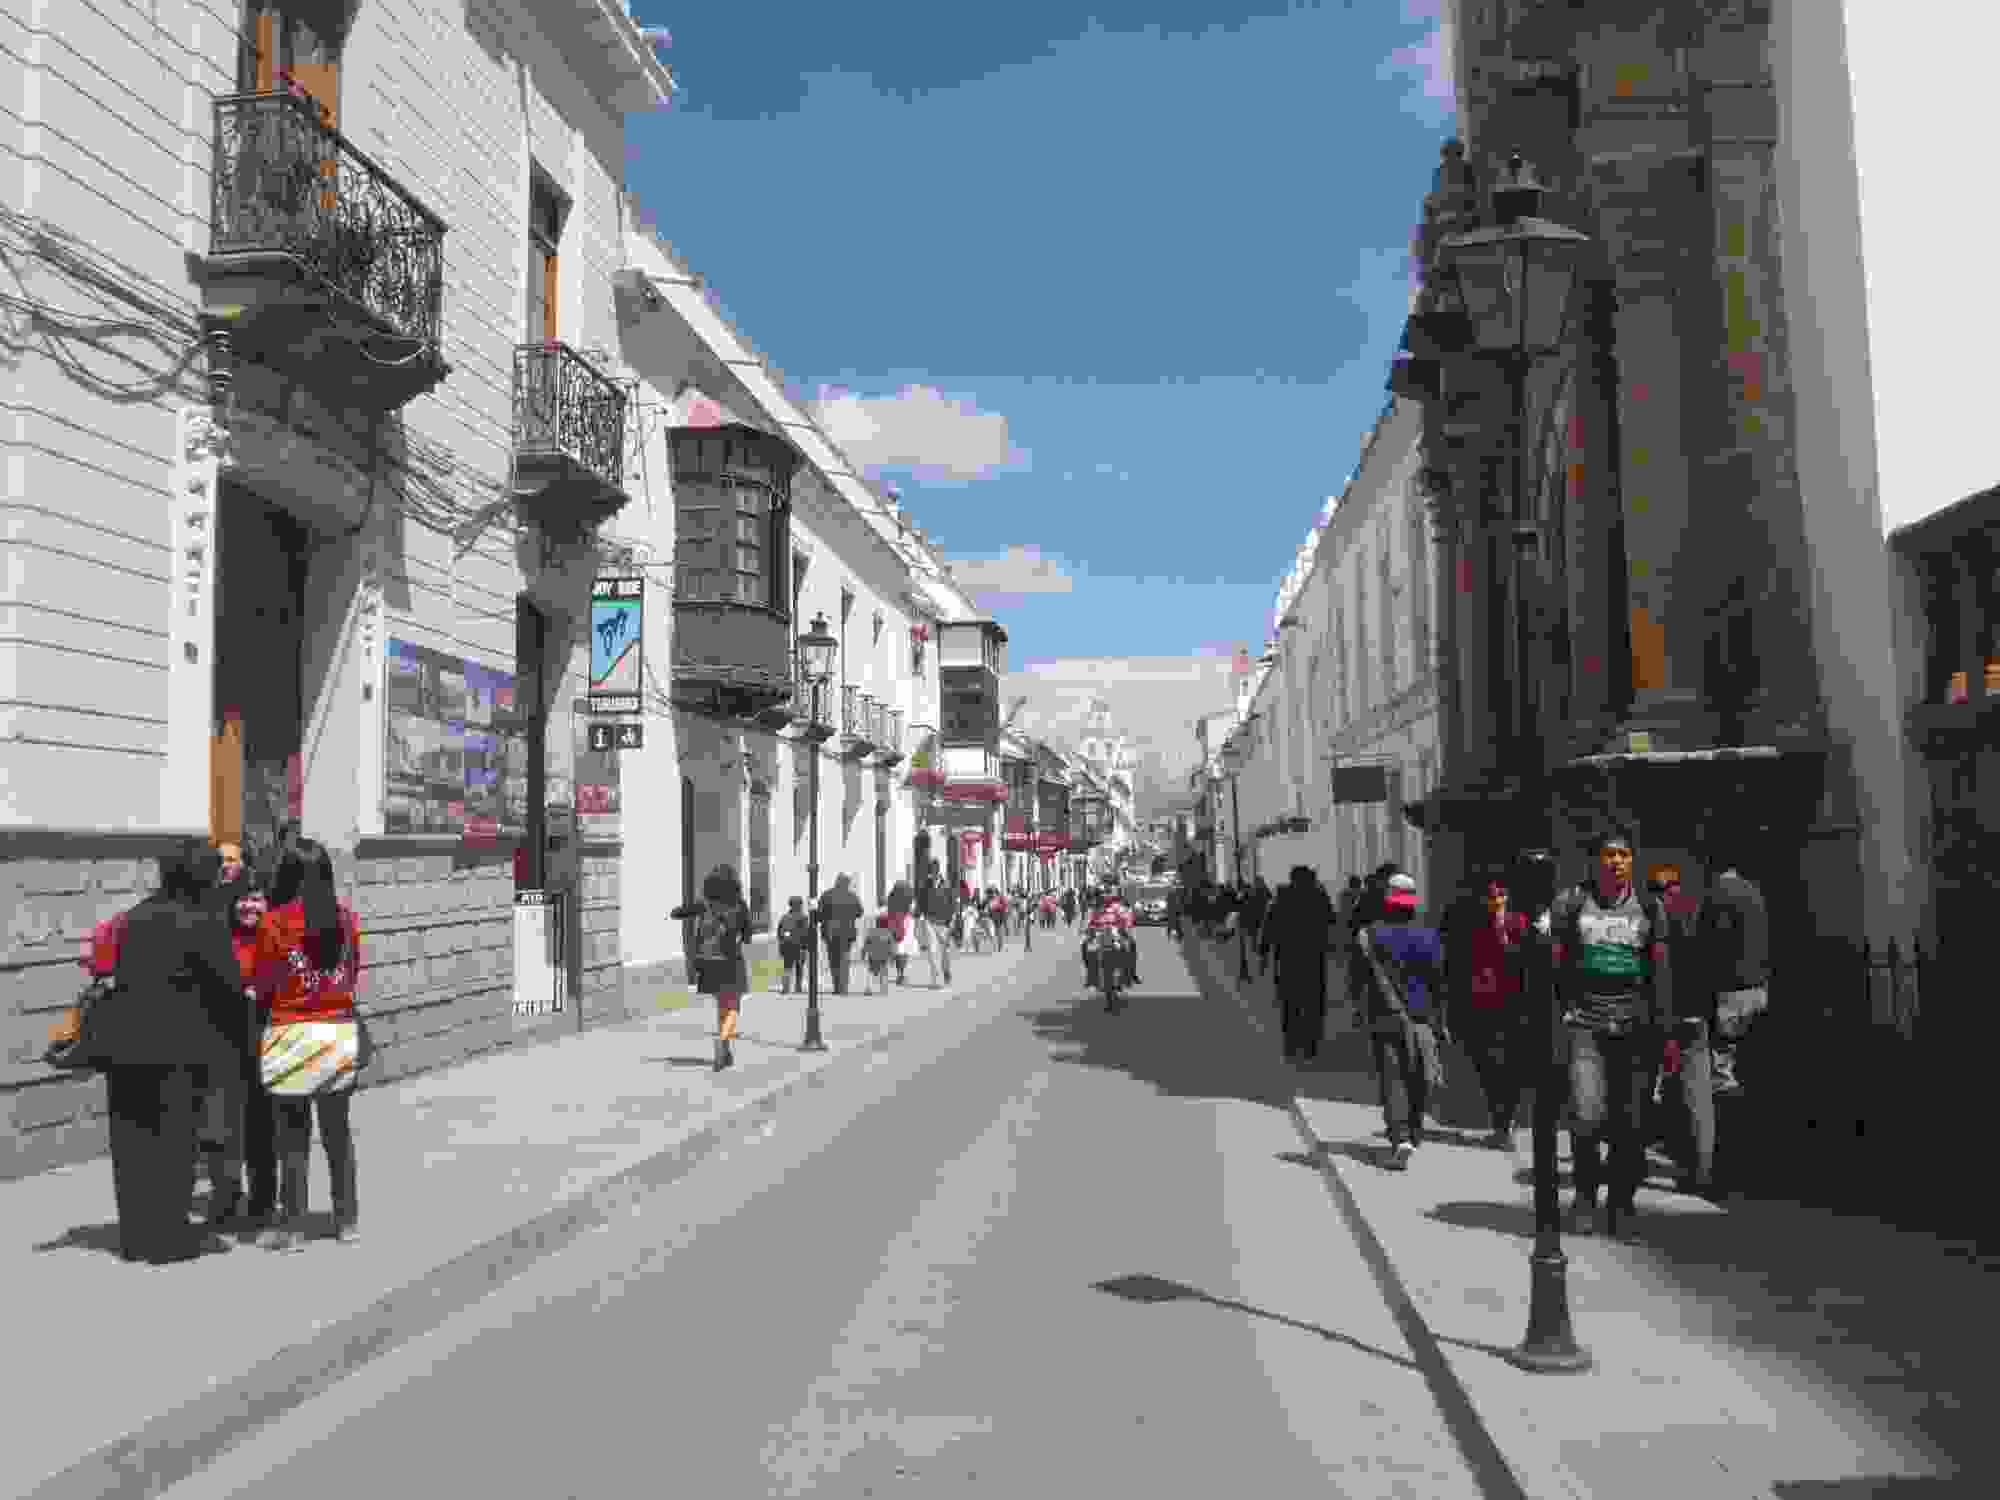
\includegraphics[width=\mywidth]{../wp-content/uploads/2015/04/wpid-wp-1429063251282.jpg} } 
 \newline
 La Plaza 25 de Mayo \newline
 \newline
\centerline{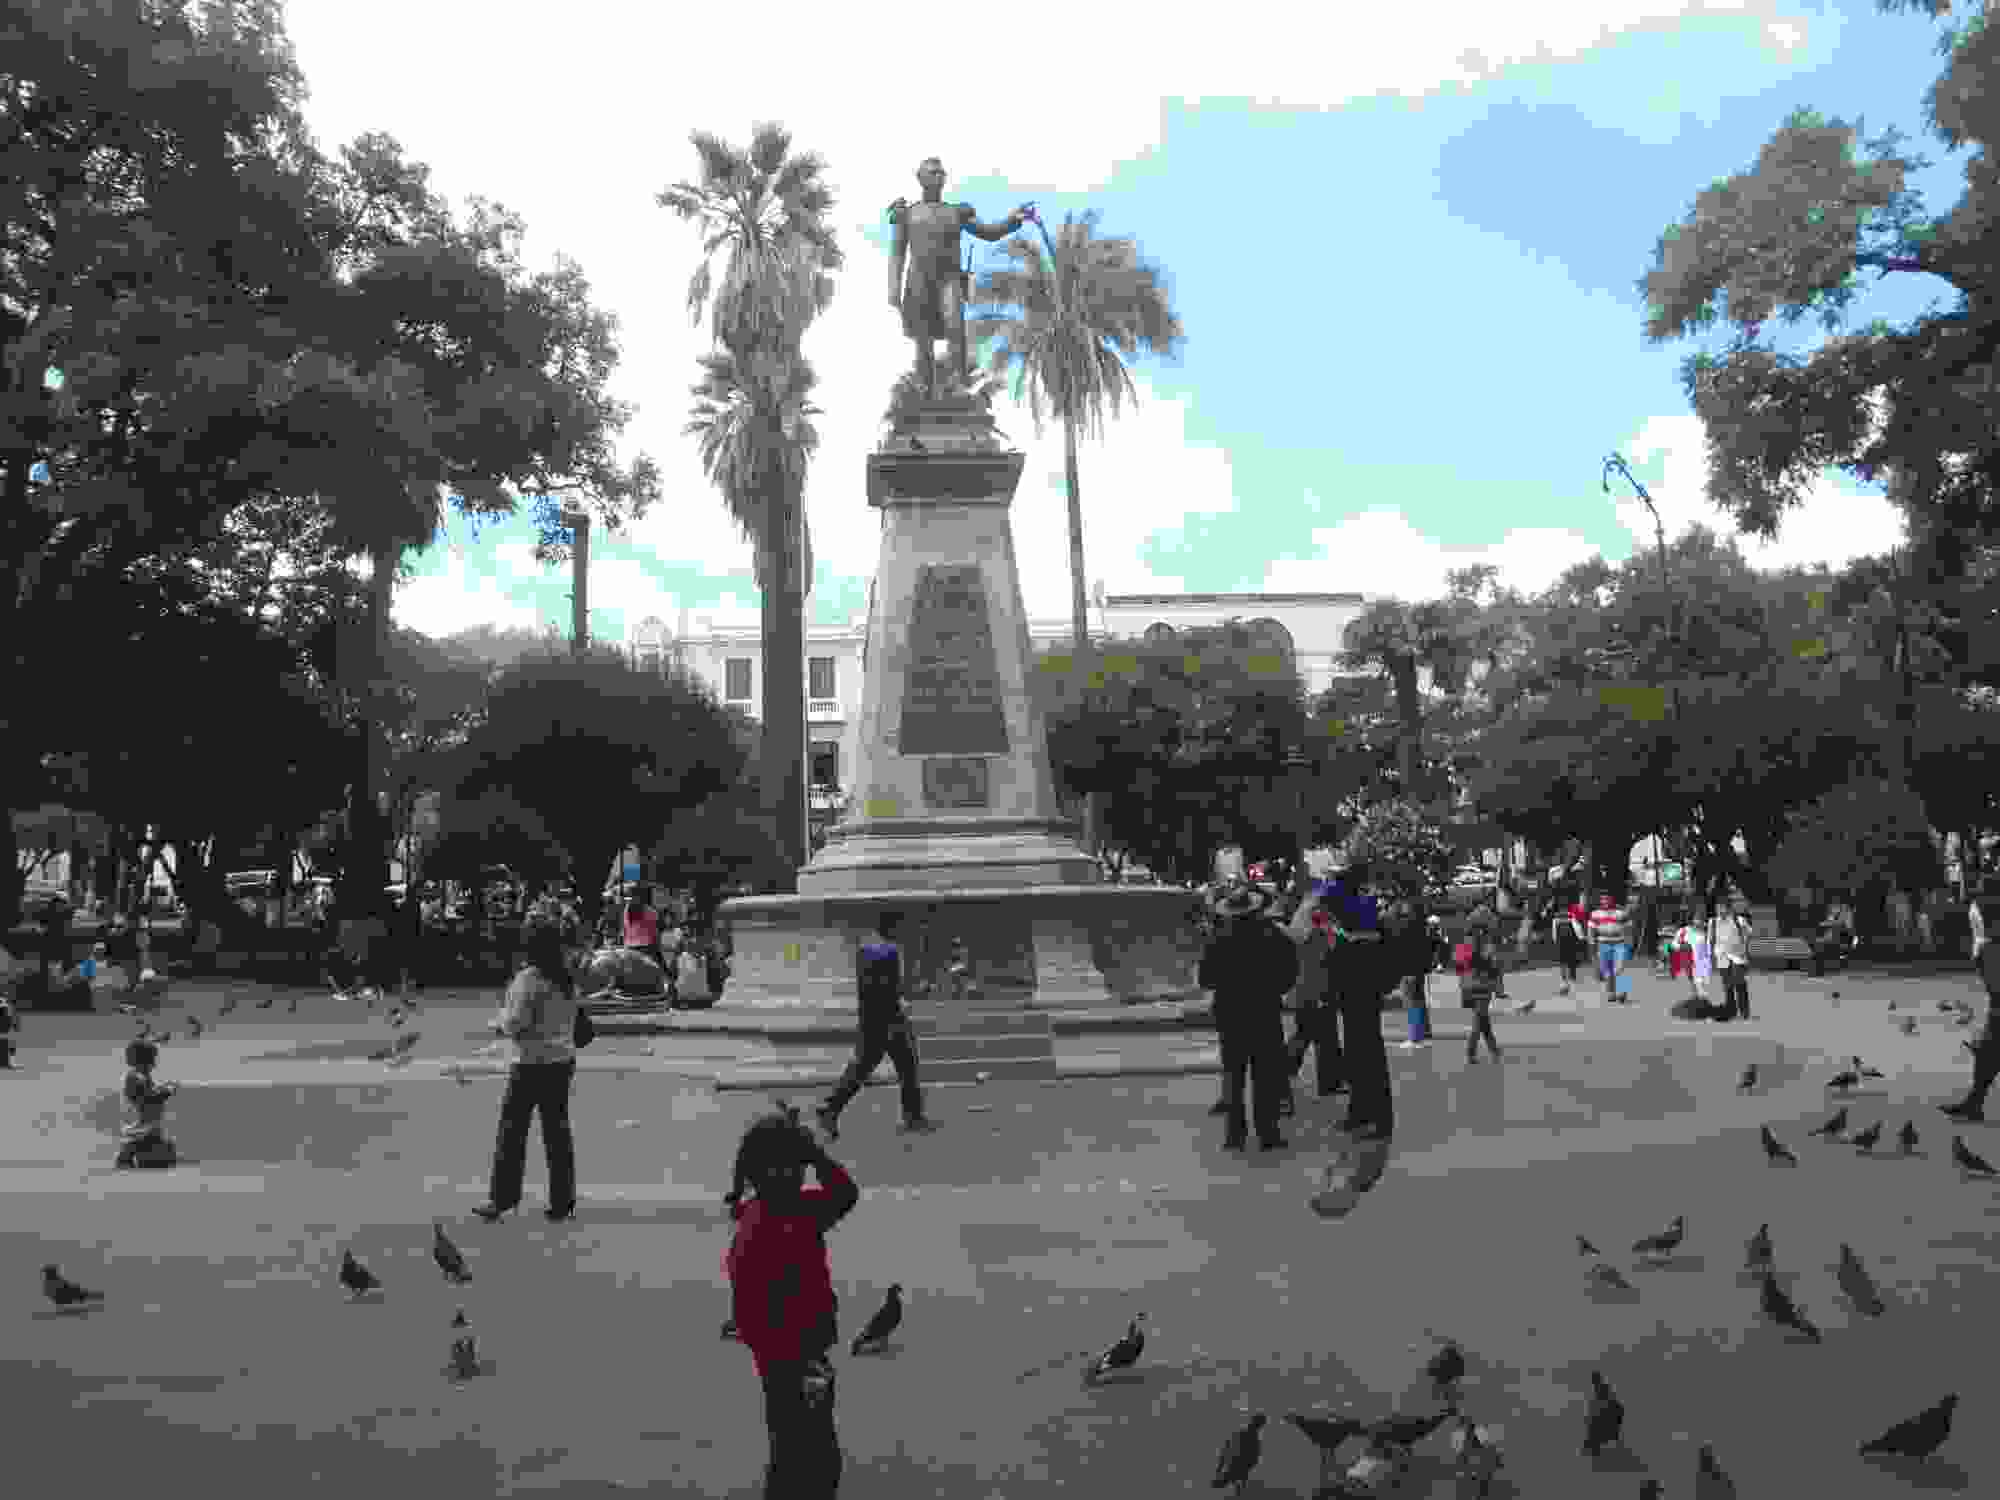
\includegraphics[width=\mywidth]{../wp-content/uploads/2015/04/wpid-wp-1429063361085.jpg} } 
 \newline
 \newline
\centerline{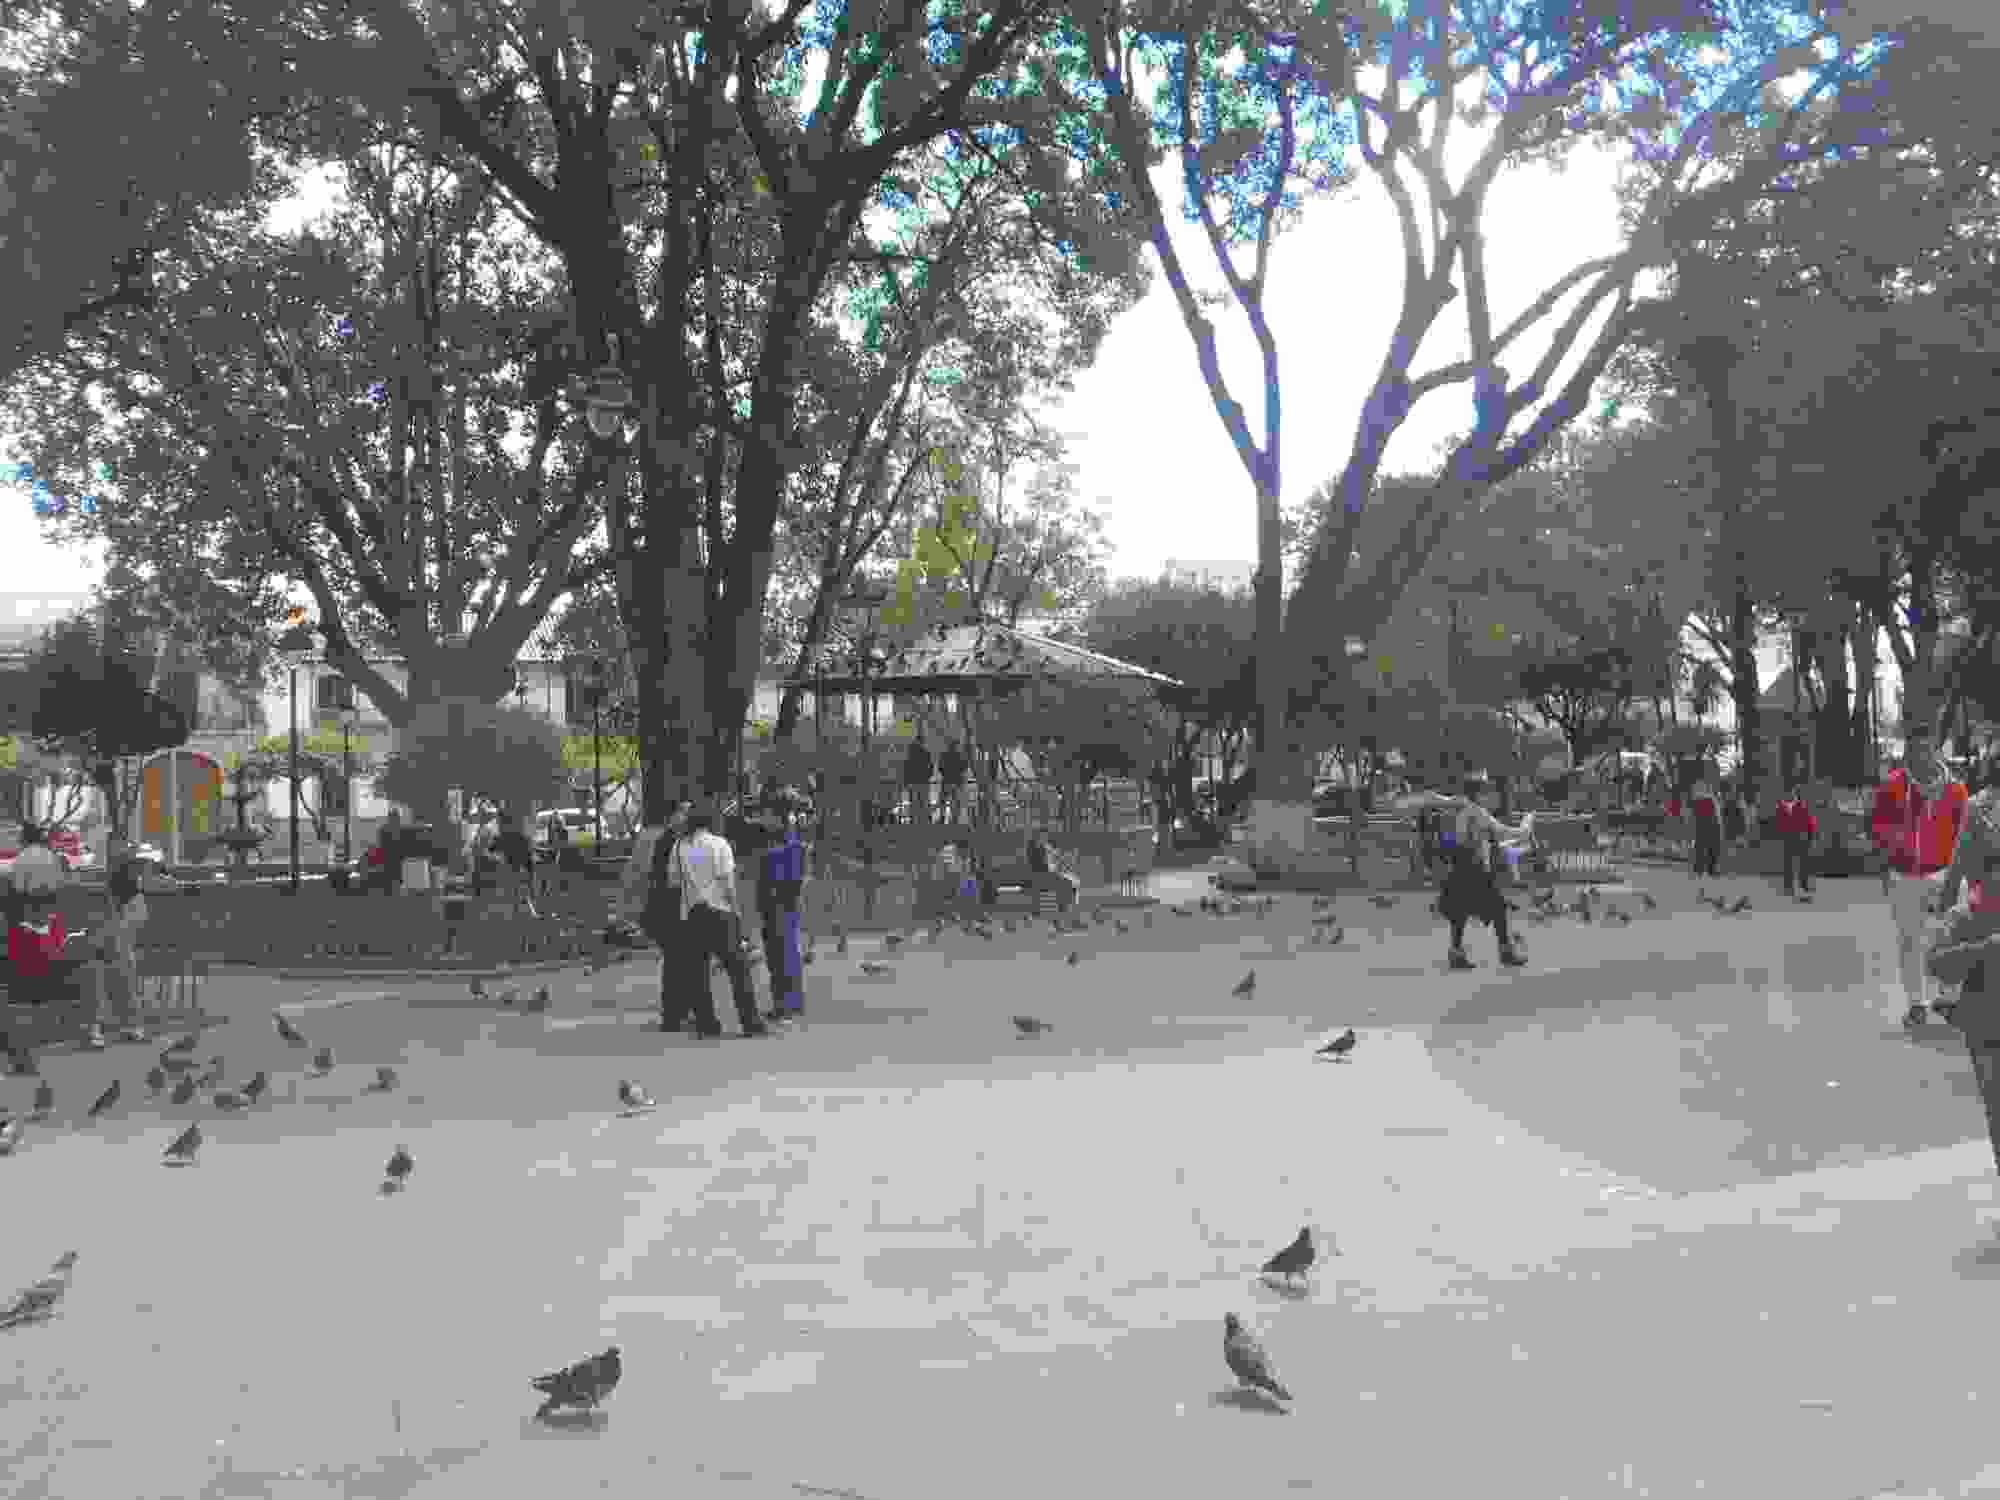
\includegraphics[width=\mywidth]{../wp-content/uploads/2015/04/wpid-wp-1429063375686.jpg} } 
 \newline
 La Casa de la Libertad : la visite explique l'histoire de l'indépendance de la Bolivie avec notamment son premier président Simon Bolivar qui a inspiré le nom du pays.  \newline
 \newline
\centerline{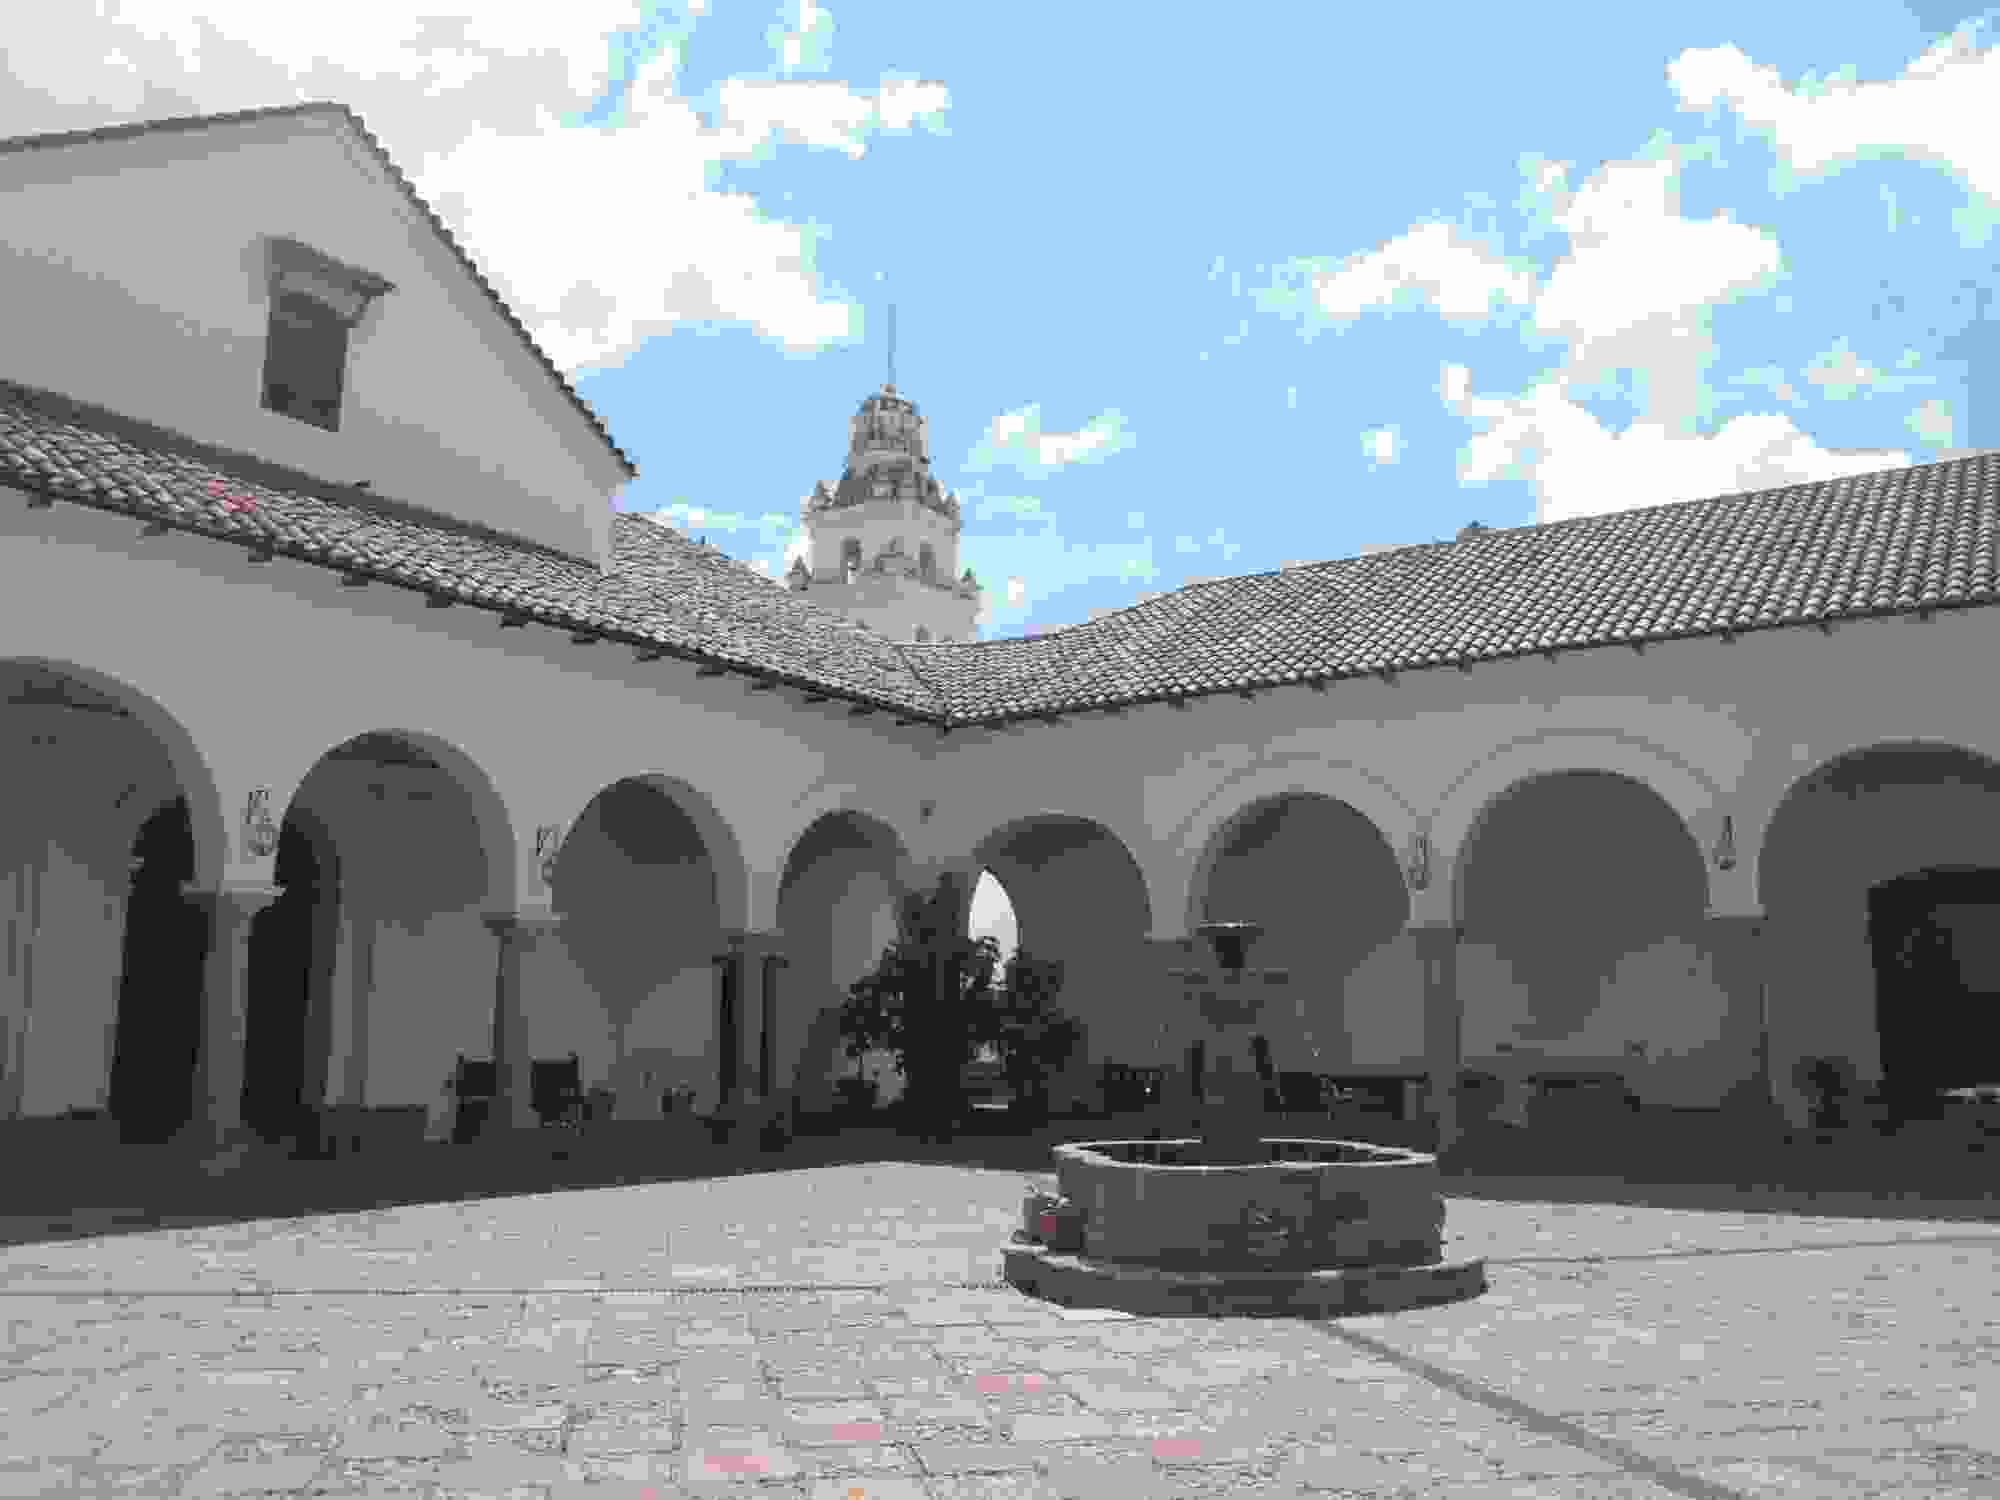
\includegraphics[width=\mywidth]{../wp-content/uploads/2015/04/wpid-wp-1429119927557.jpg} } 
 \newline
 \newline
\centerline{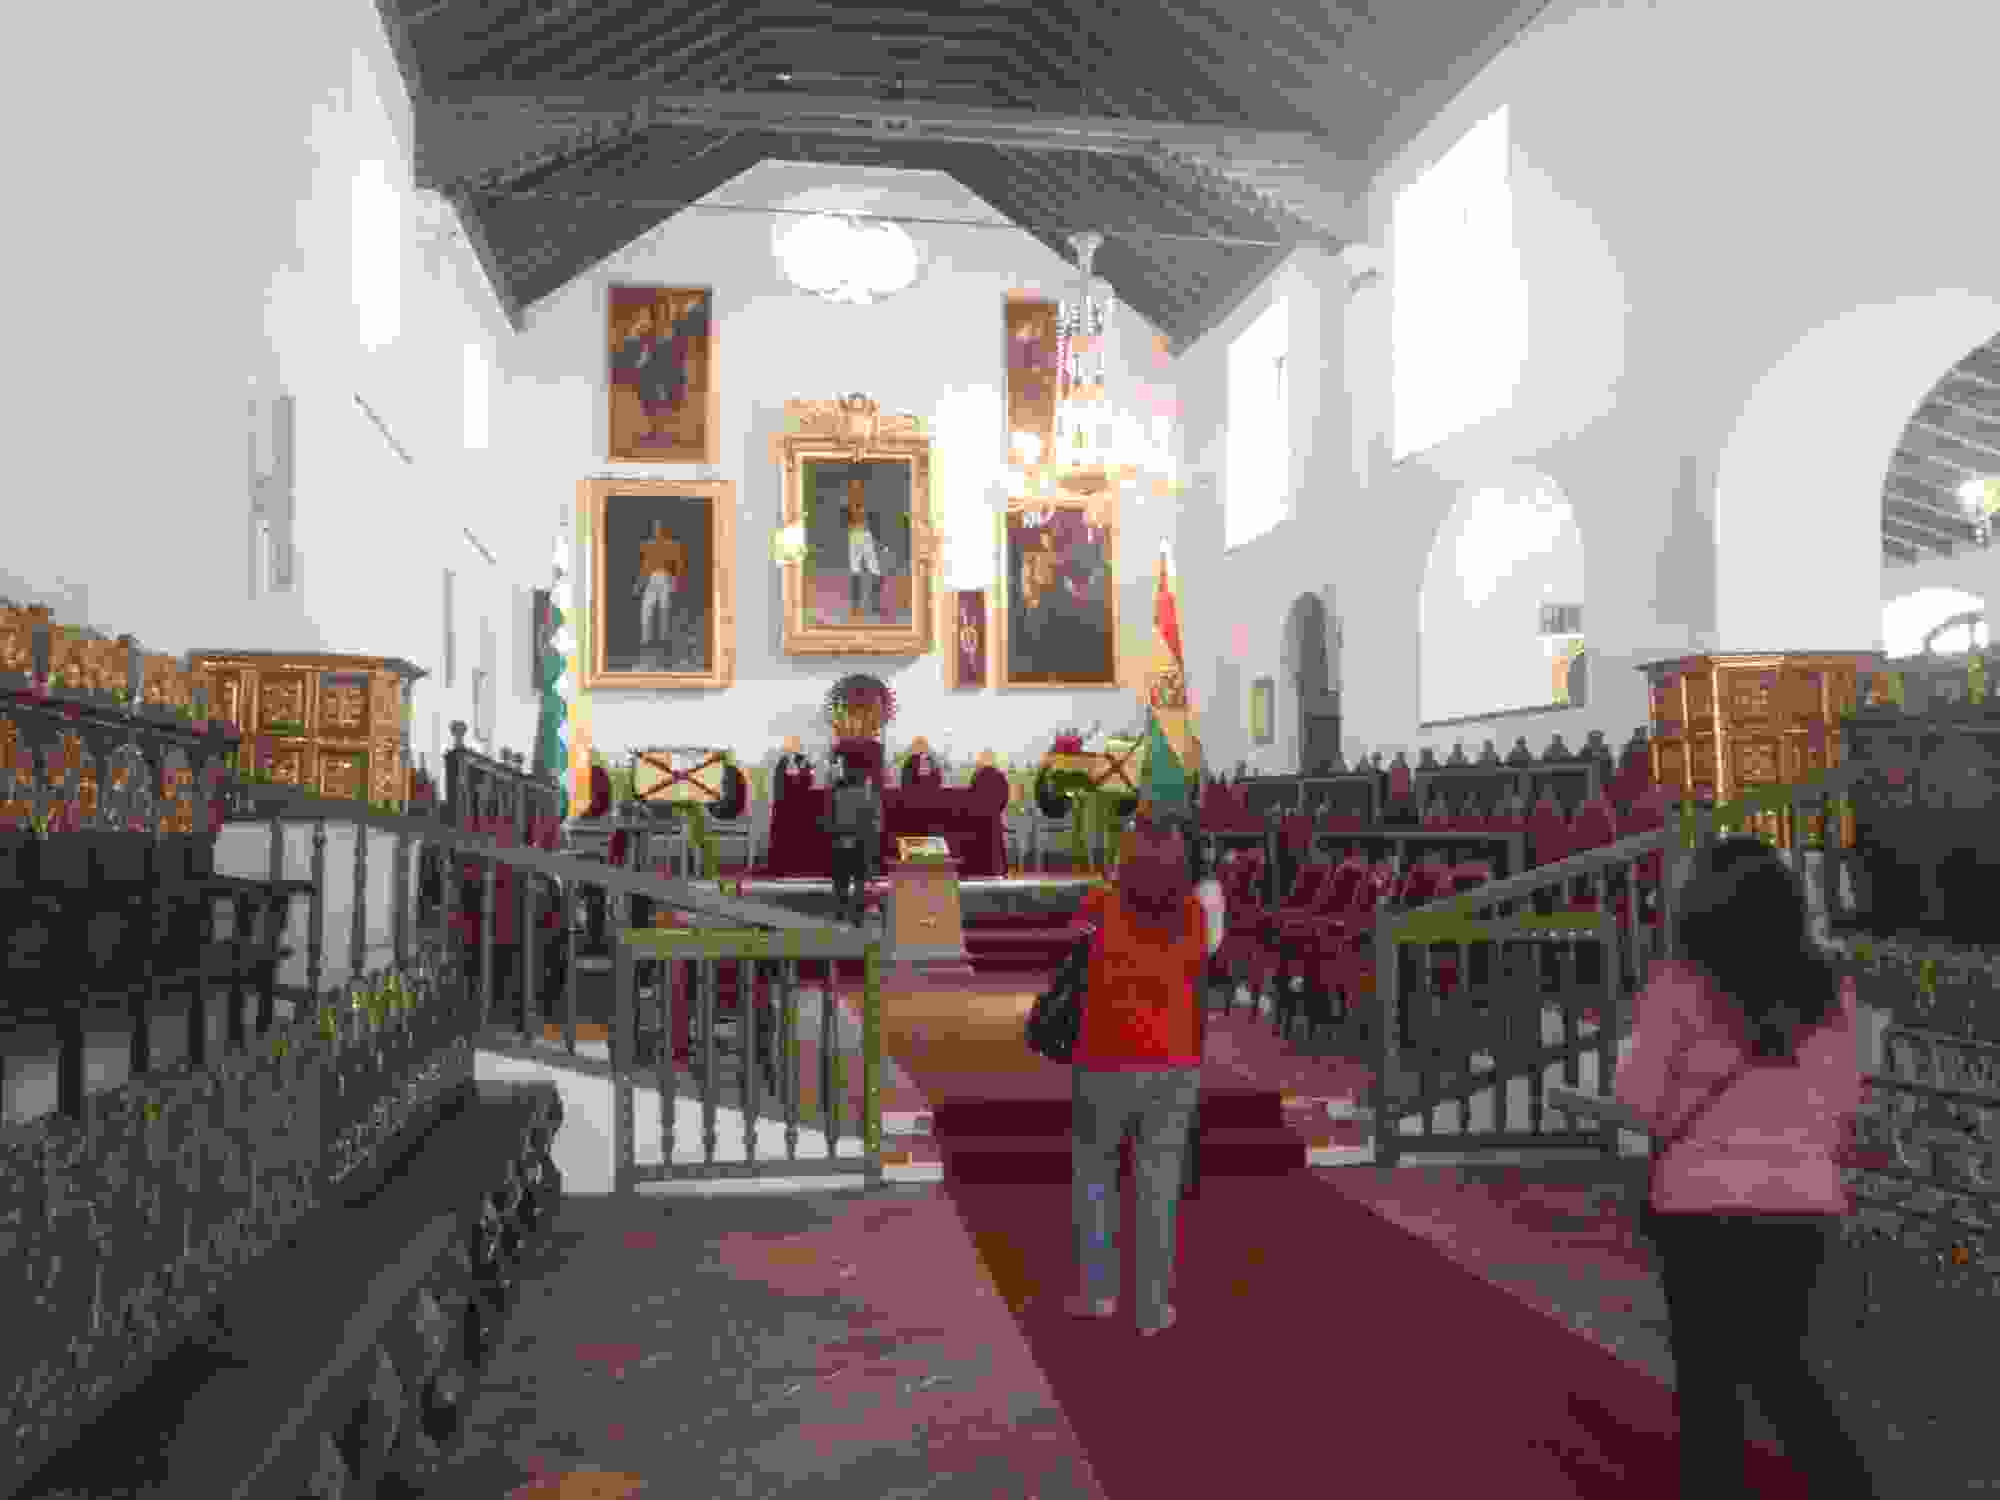
\includegraphics[width=\mywidth]{../wp-content/uploads/2015/04/wpid-wp-1429120135293.jpg} } 
 \newline
 La cathédrale et de belles églises \newline
 \newline
\centerline{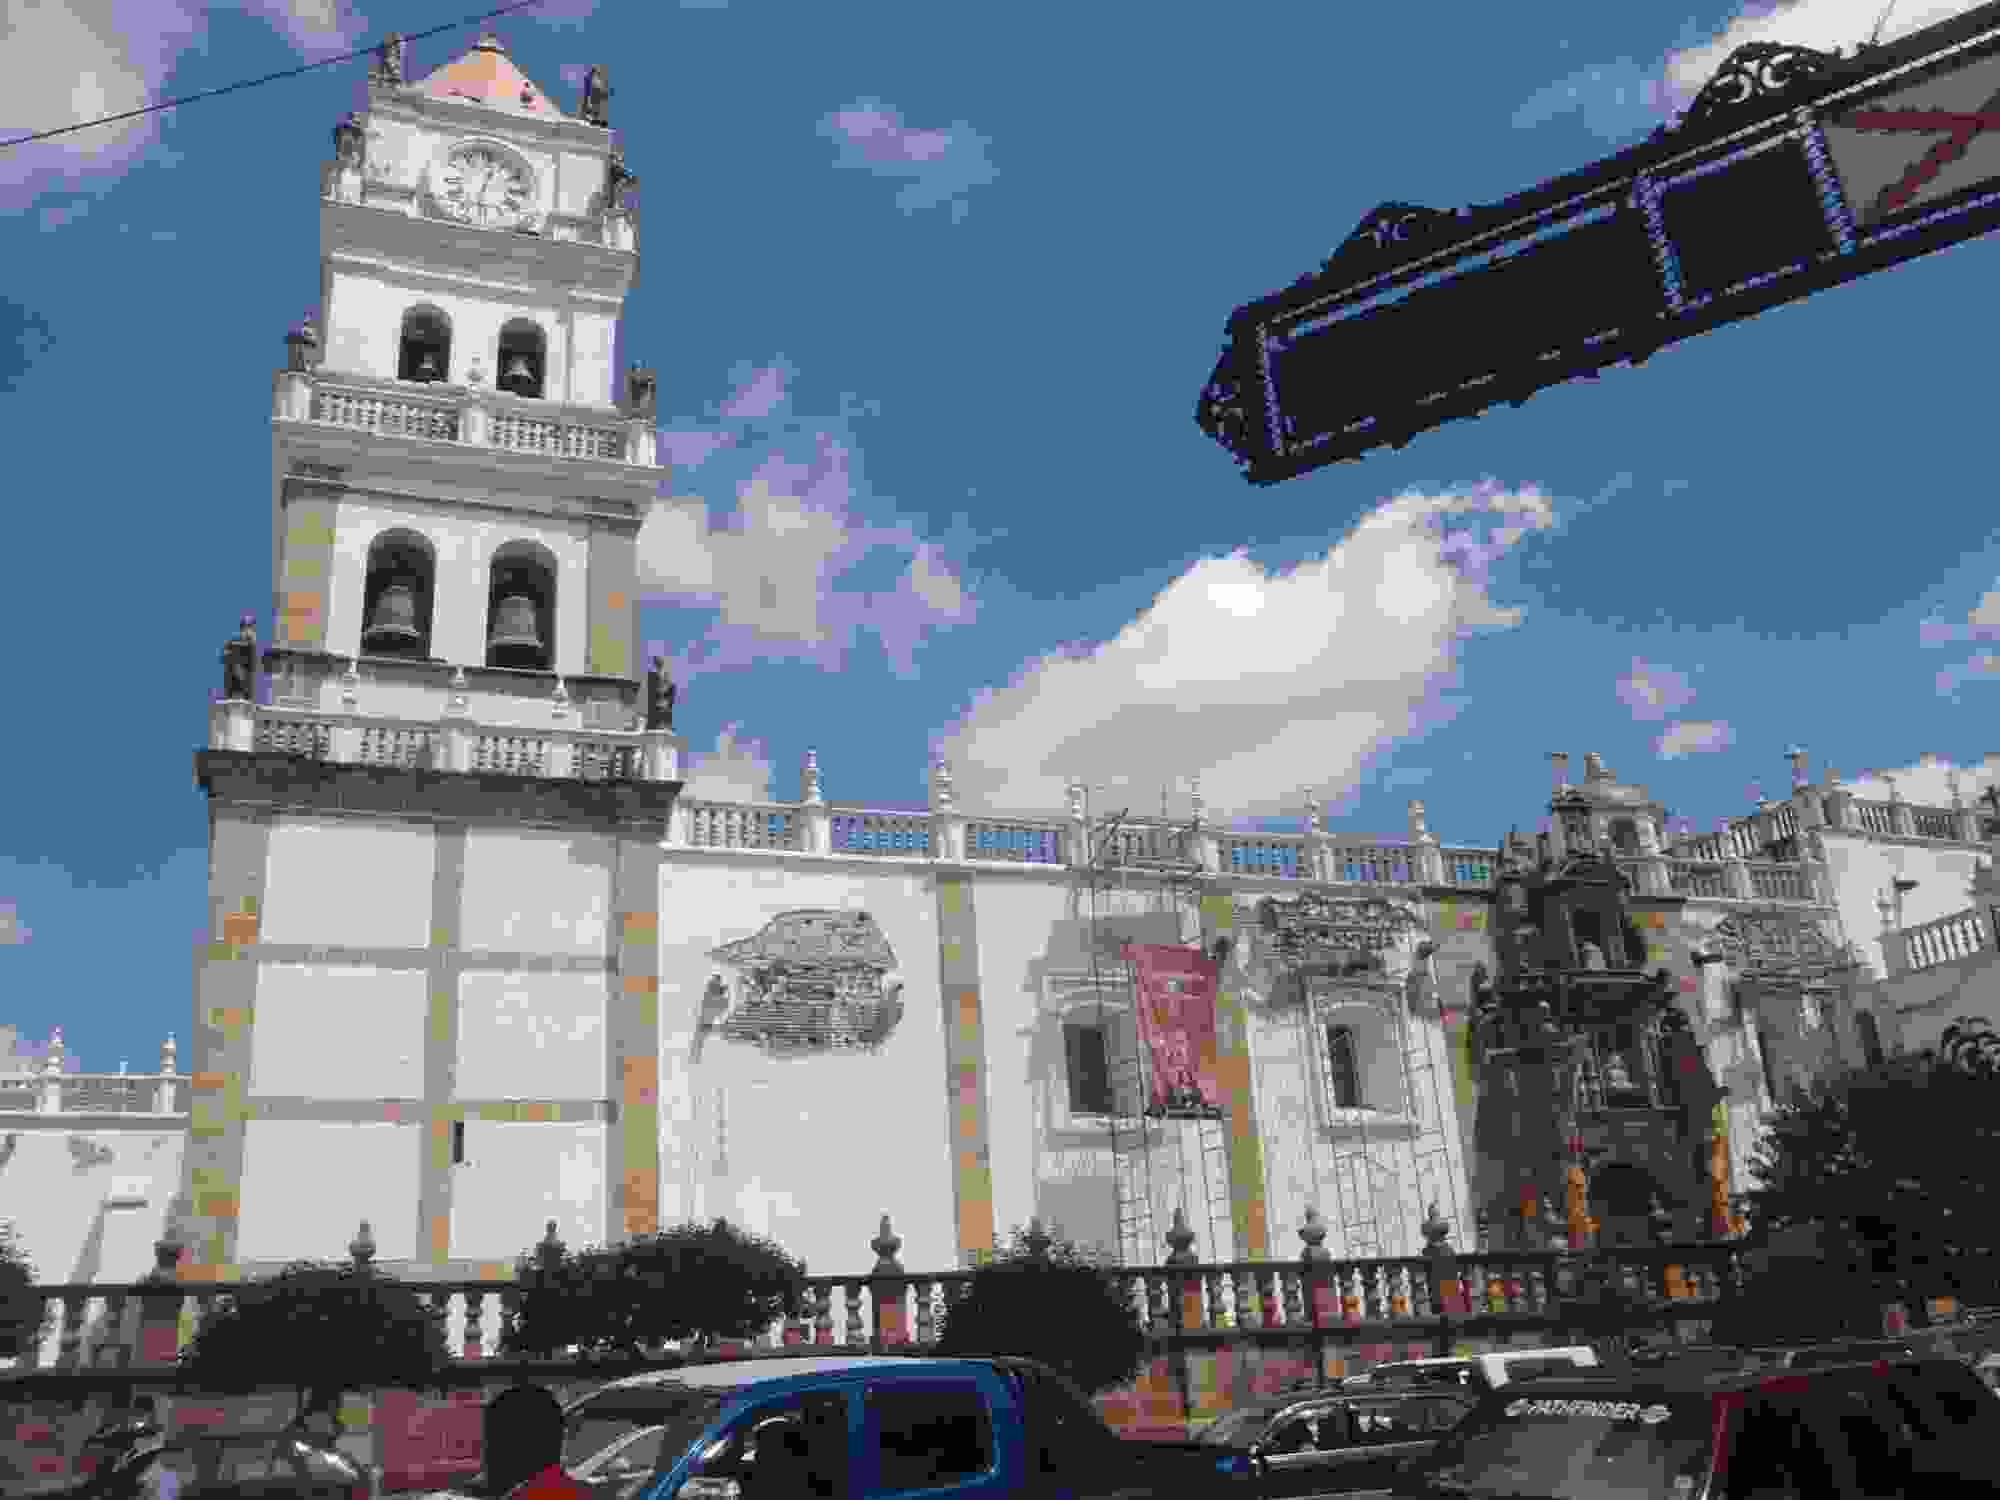
\includegraphics[width=\mywidth]{../wp-content/uploads/2015/04/wpid-wp-1429063401622.jpg} } 
 \newline
 \newline
\centerline{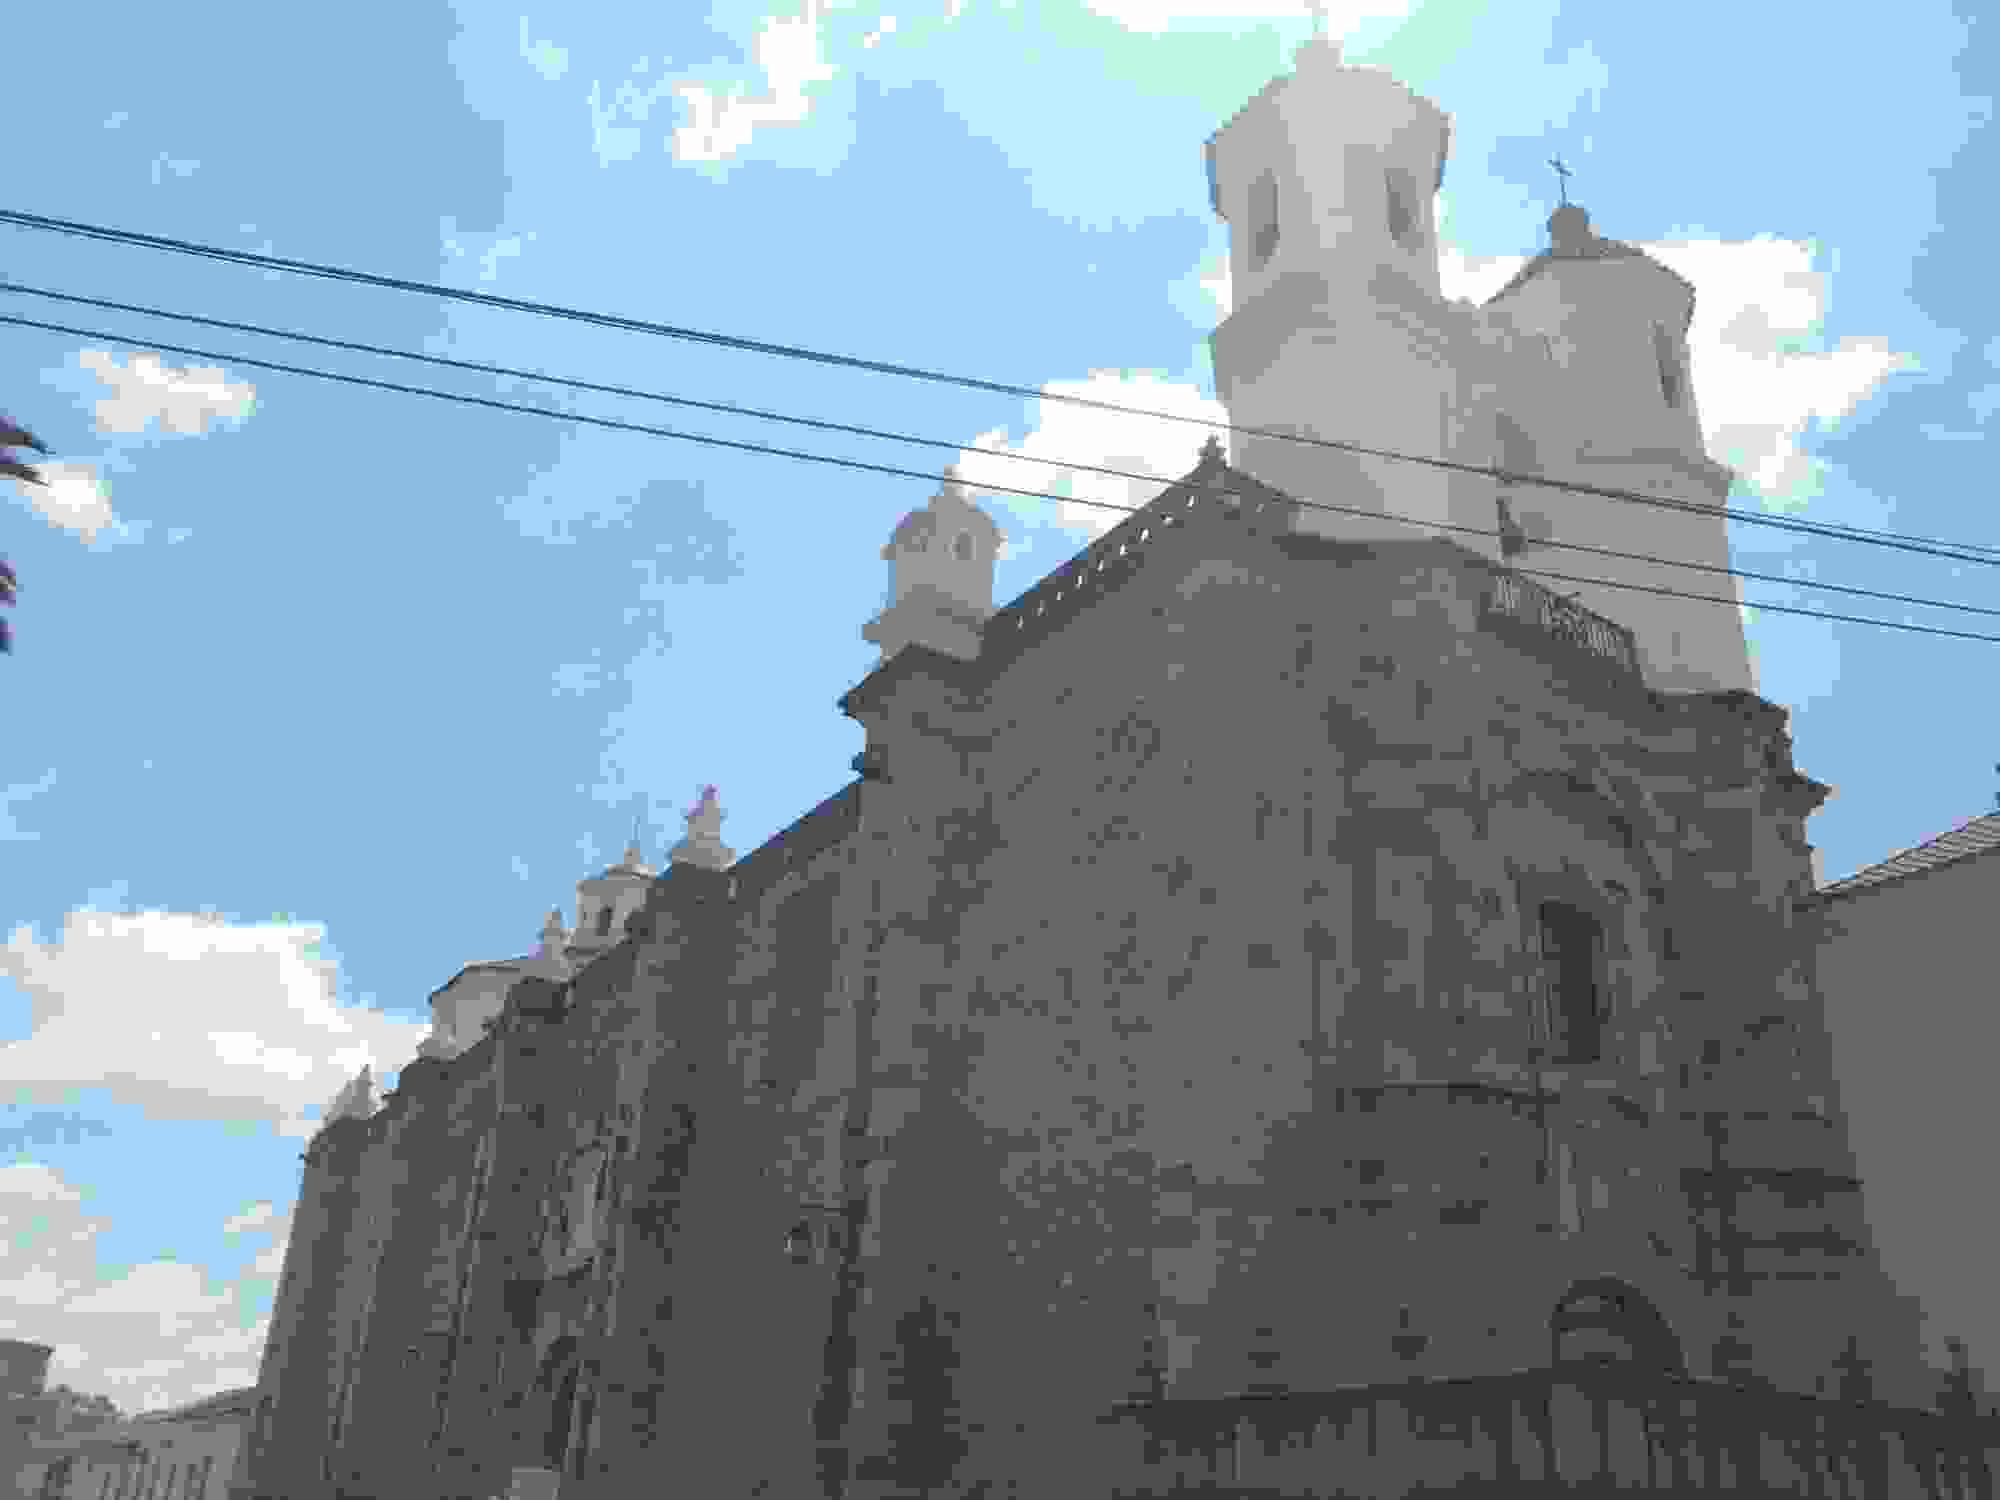
\includegraphics[width=\mywidth]{../wp-content/uploads/2015/04/wpid-wp-1429063437281.jpg} } 
 \newline
 \newline
\centerline{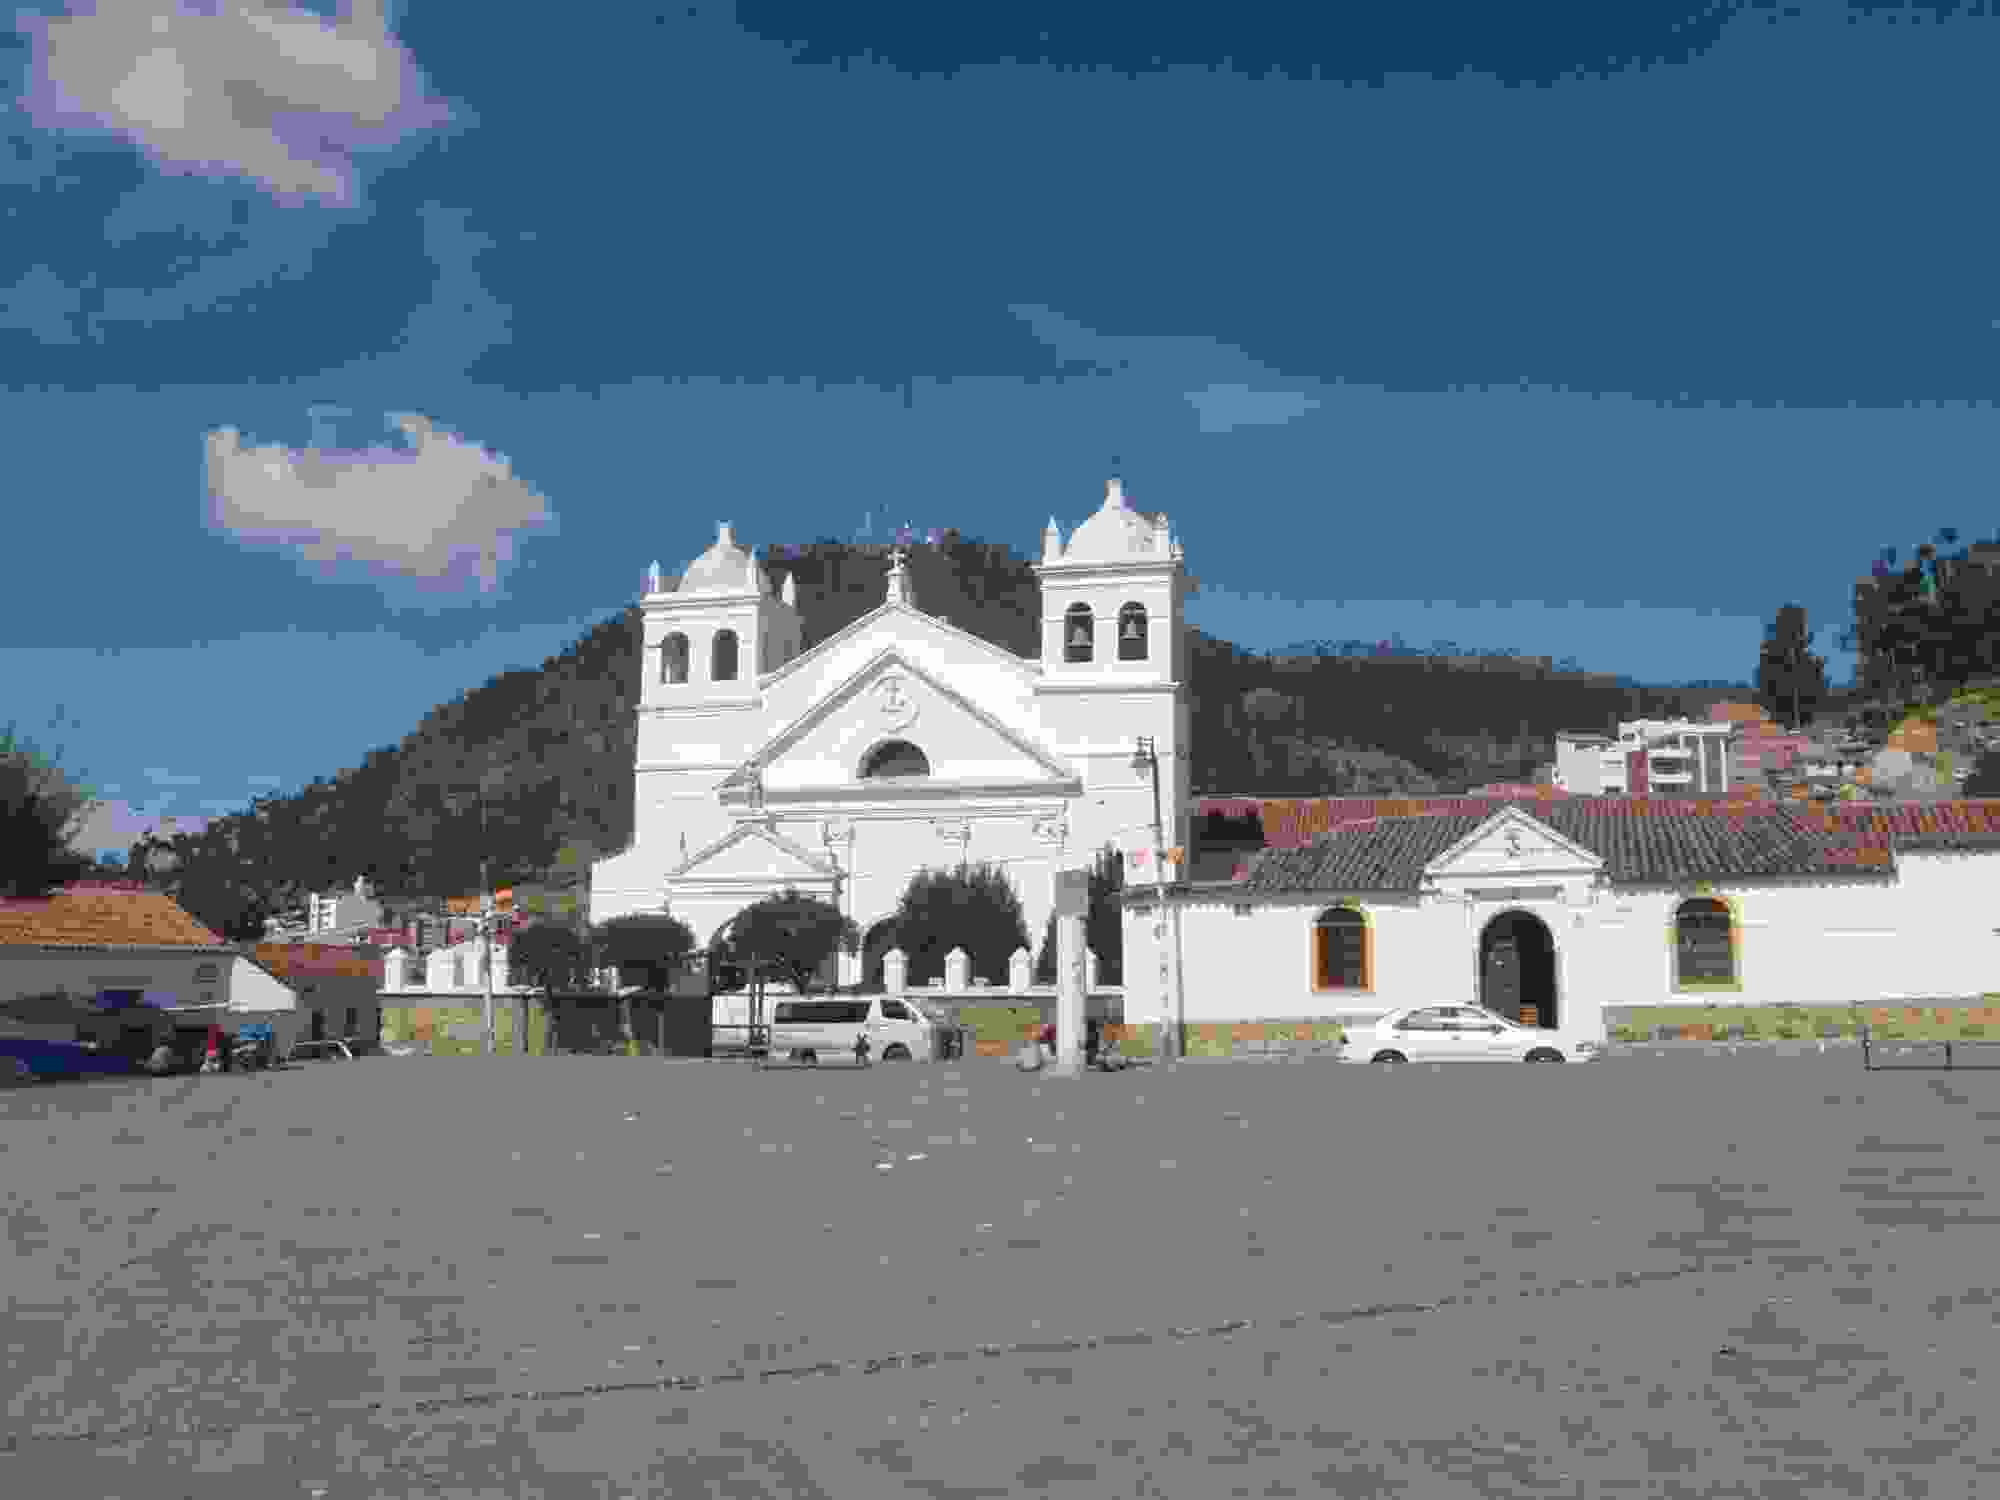
\includegraphics[width=\mywidth]{../wp-content/uploads/2015/04/wpid-wp-1429063894588.jpg} } 
 \newline
 Le marché central de Sucre, une merveille on trouve de tout.  \newline
 \newline
\centerline{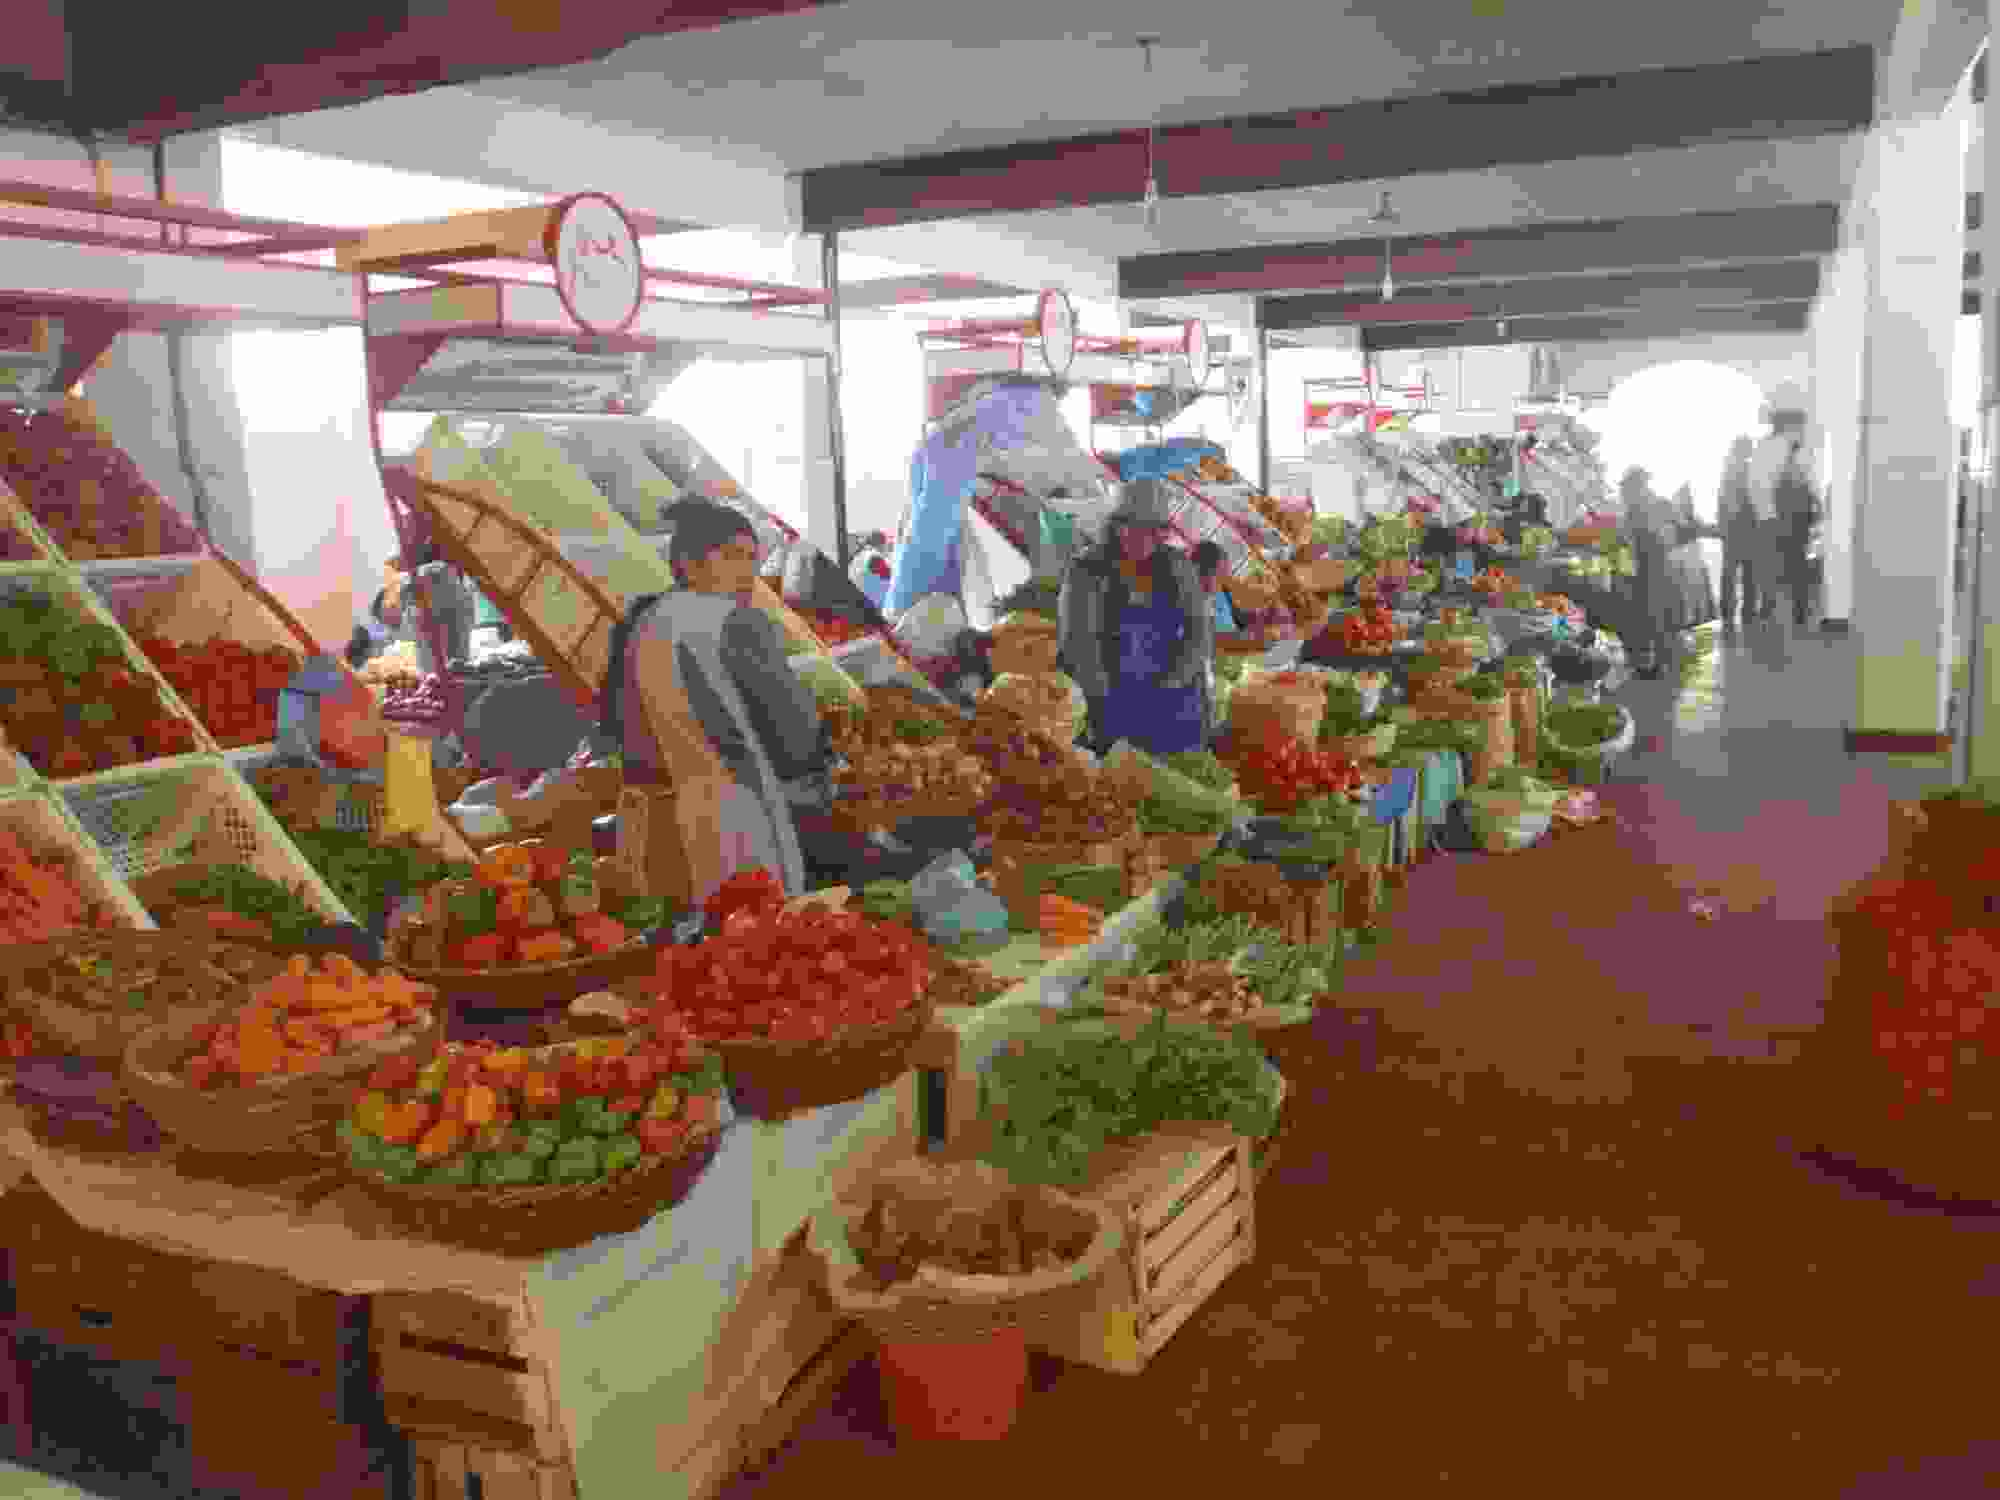
\includegraphics[width=\mywidth]{../wp-content/uploads/2015/04/wpid-wp-1429062883937.jpg} } 
 \newline
 \newline
\centerline{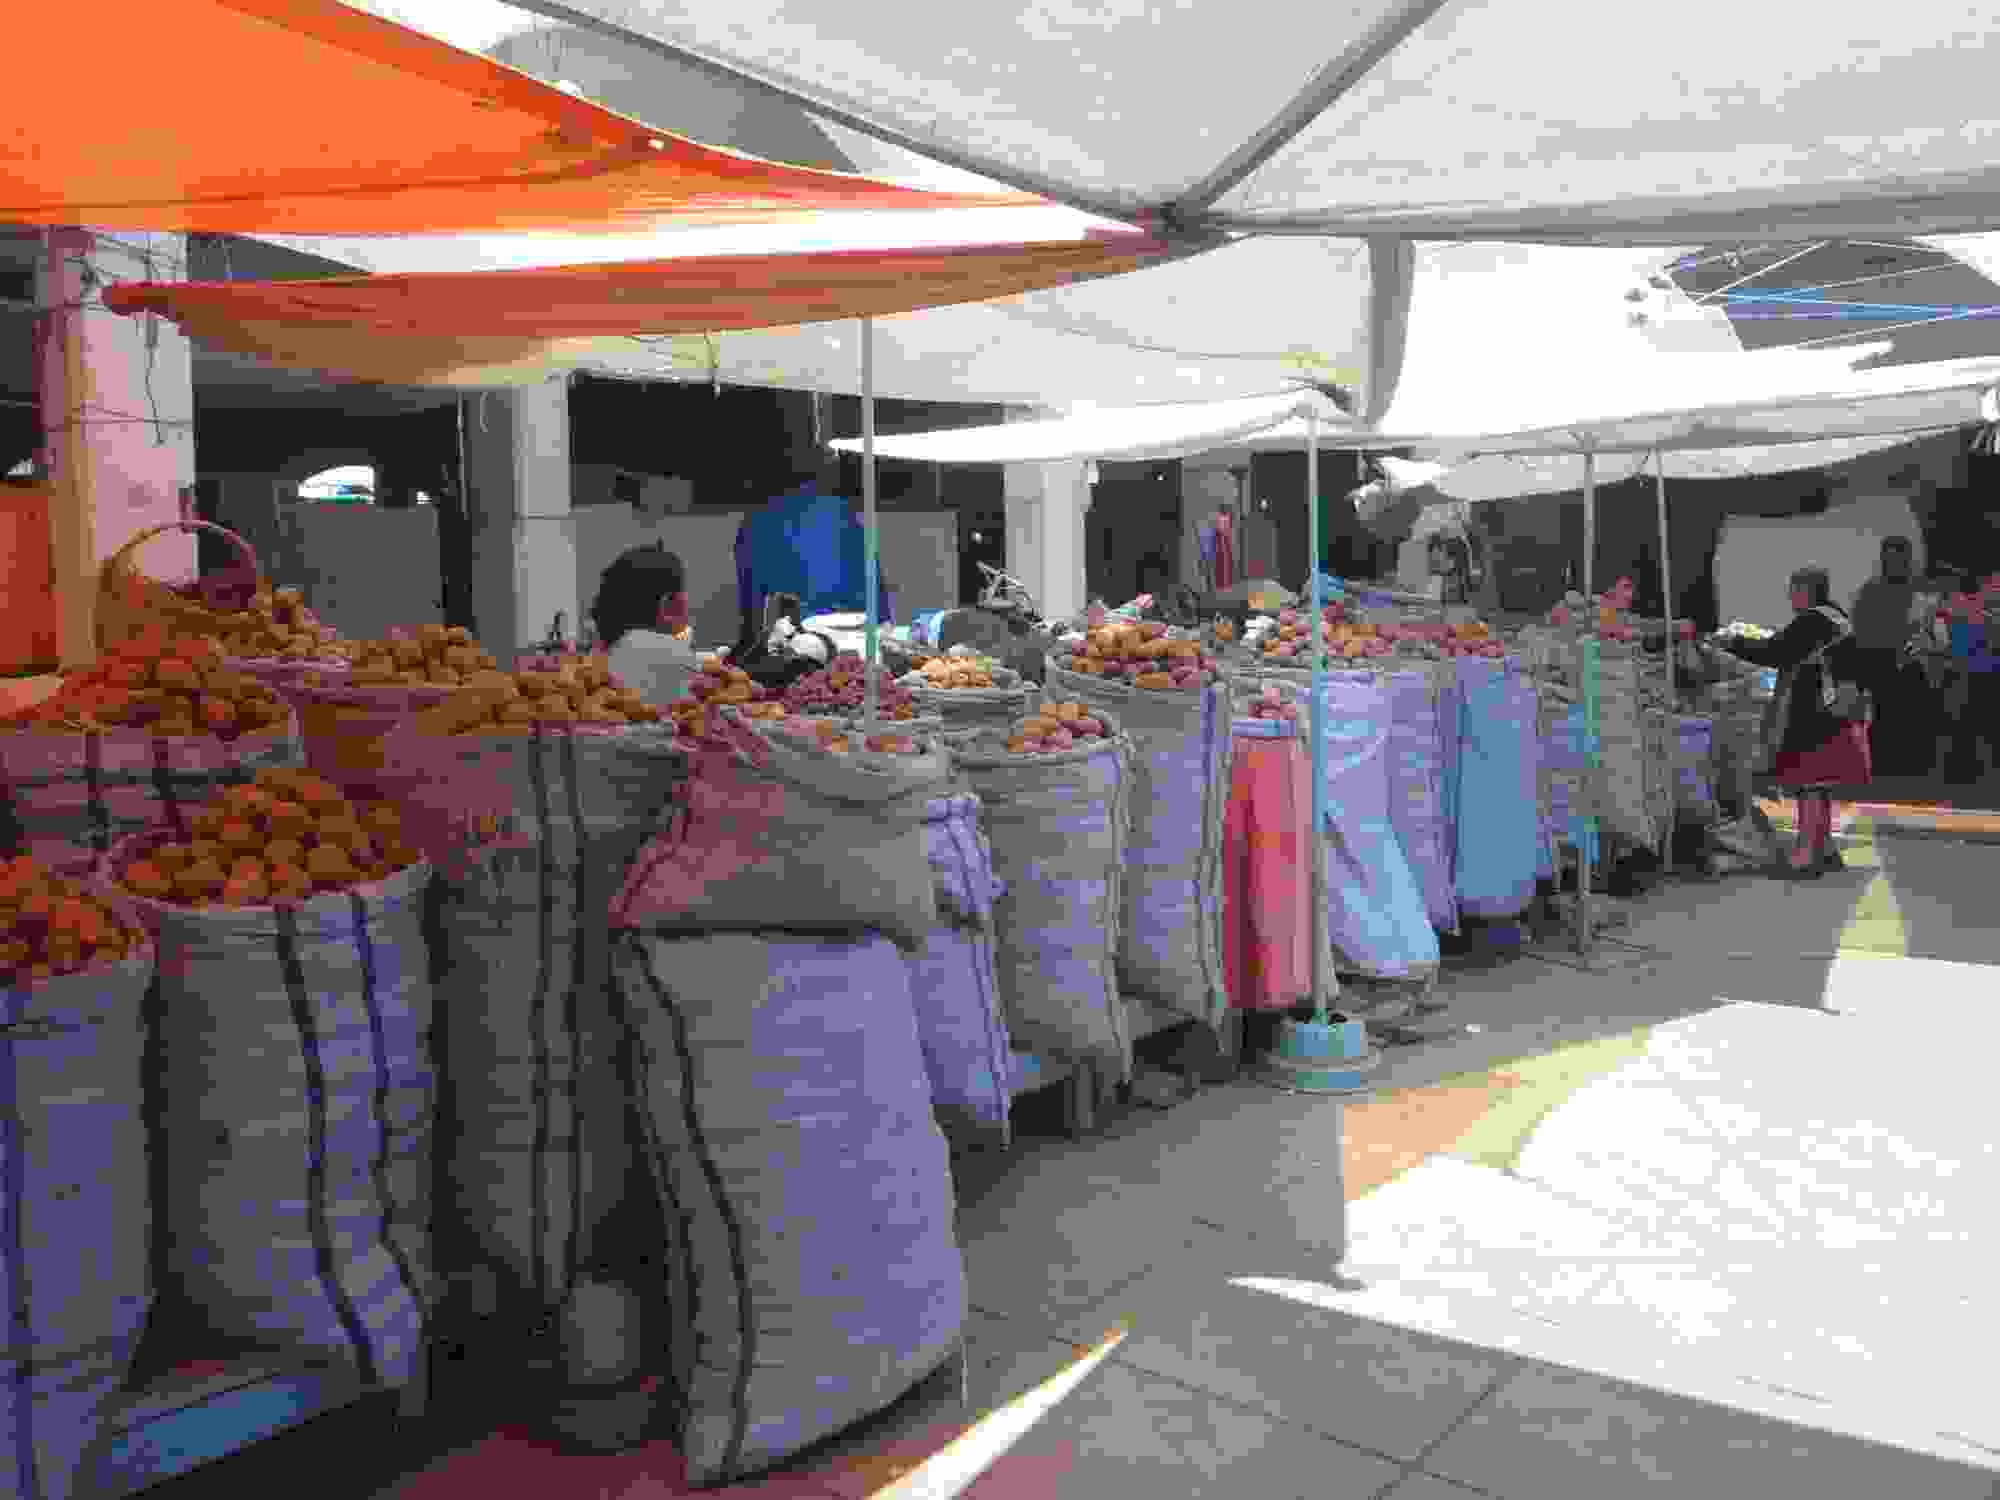
\includegraphics[width=\mywidth]{../wp-content/uploads/2015/04/wpid-wp-1429062898209.jpg} } 
 \newline
 \newline
\centerline{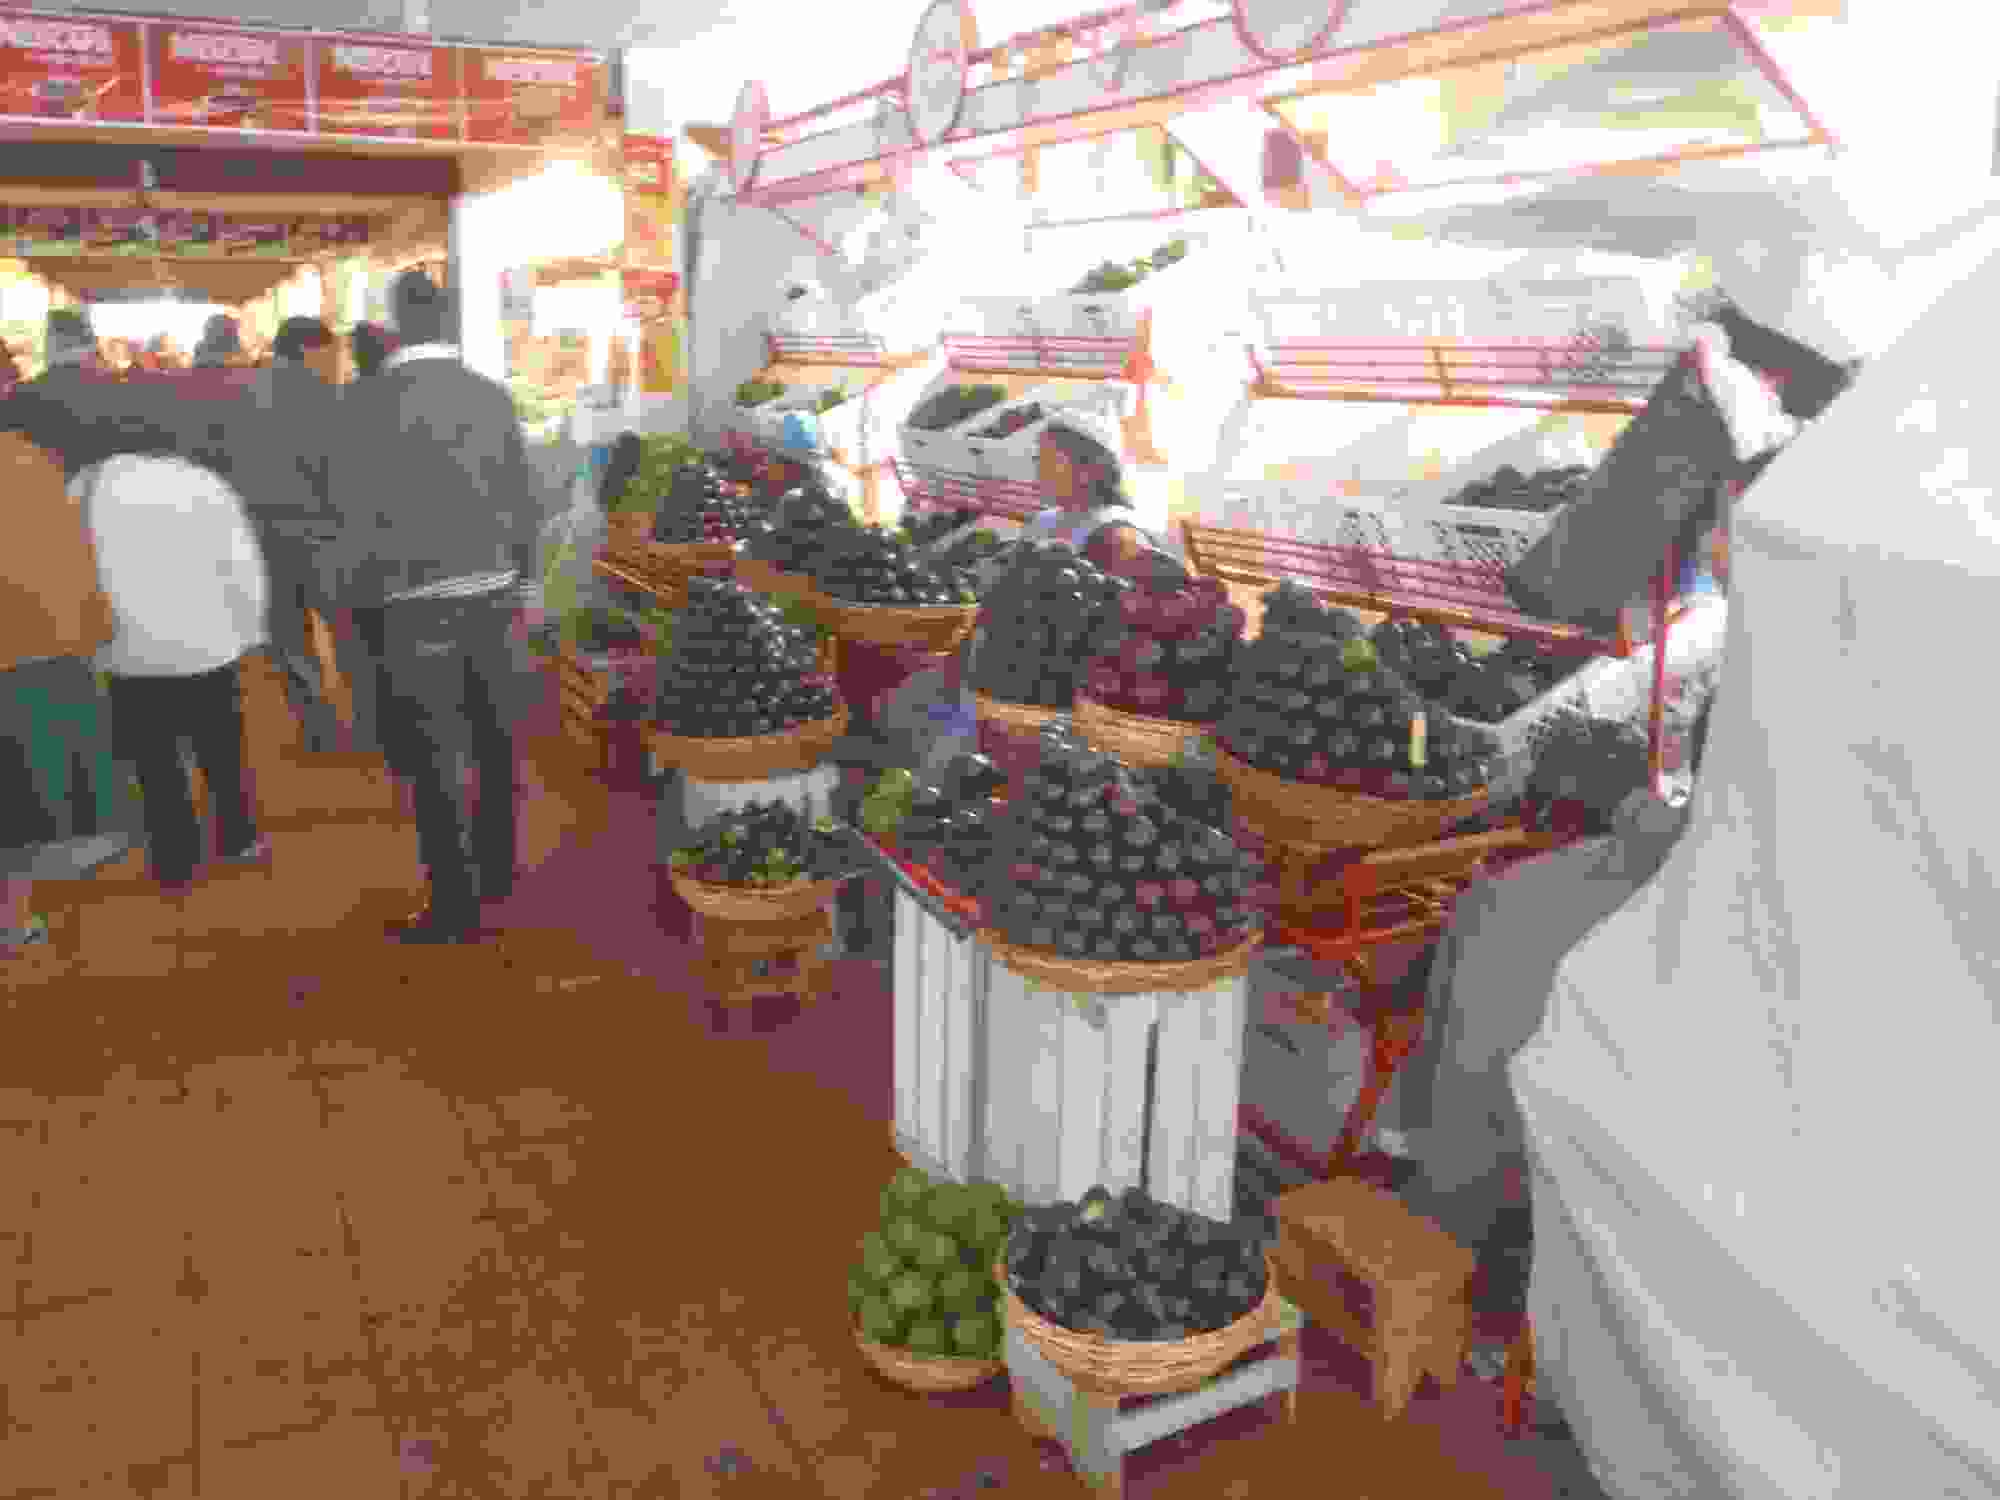
\includegraphics[width=\mywidth]{../wp-content/uploads/2015/04/wpid-wp-1429062910596.jpg} } 
 \newline
 \newline
\centerline{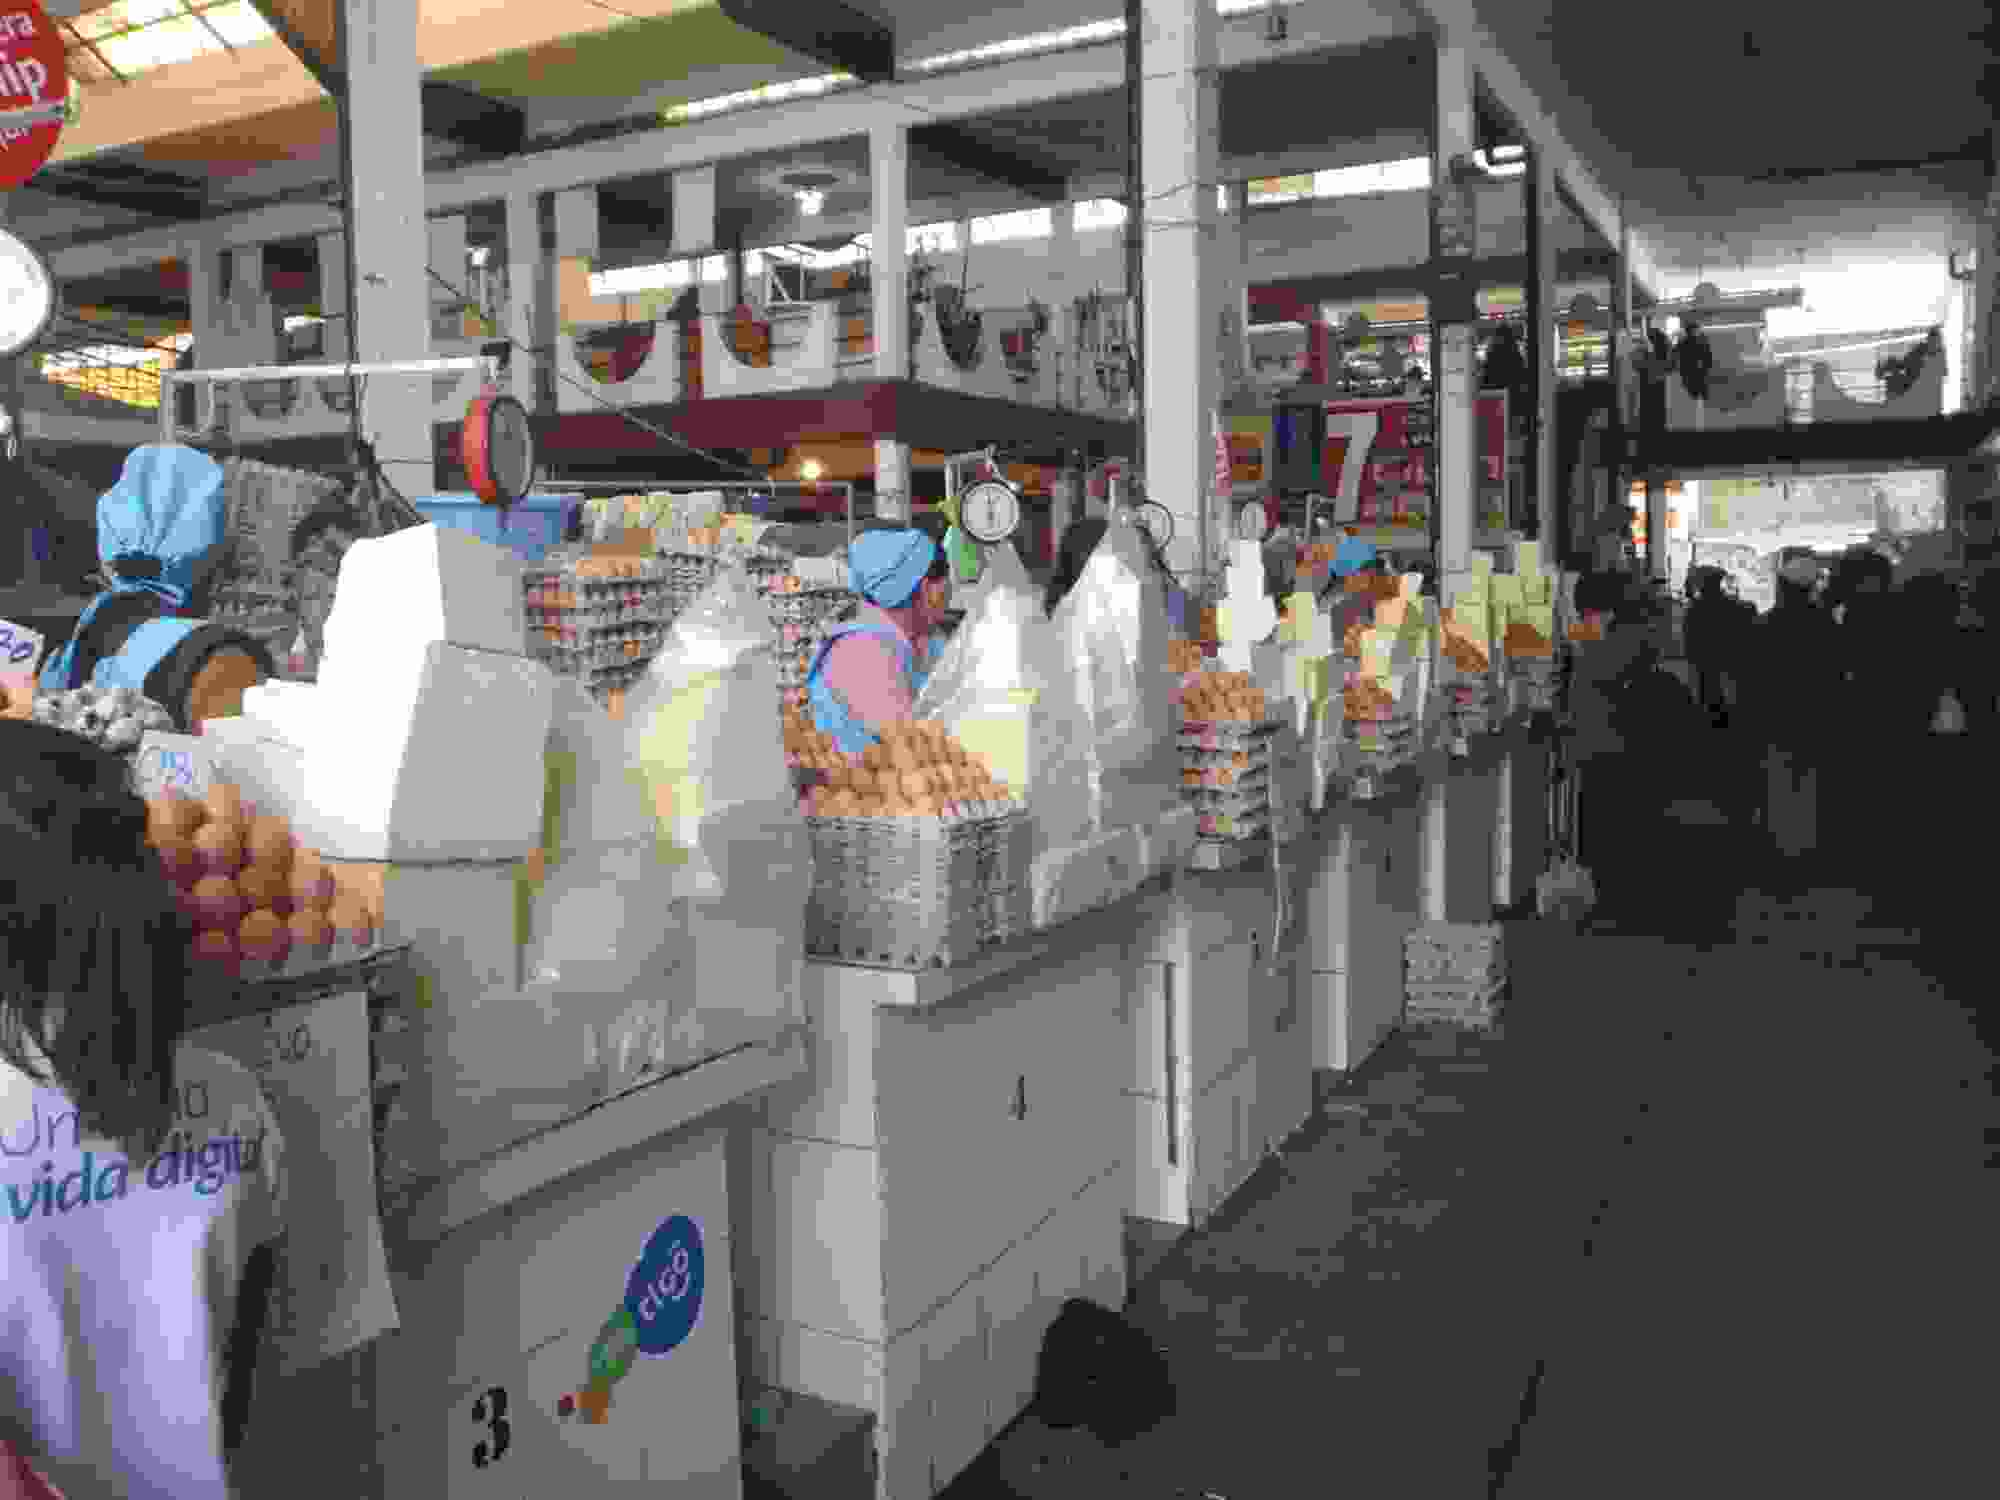
\includegraphics[width=\mywidth]{../wp-content/uploads/2015/04/wpid-wp-1429062969618.jpg} } 
 \newline
 \newline
\centerline{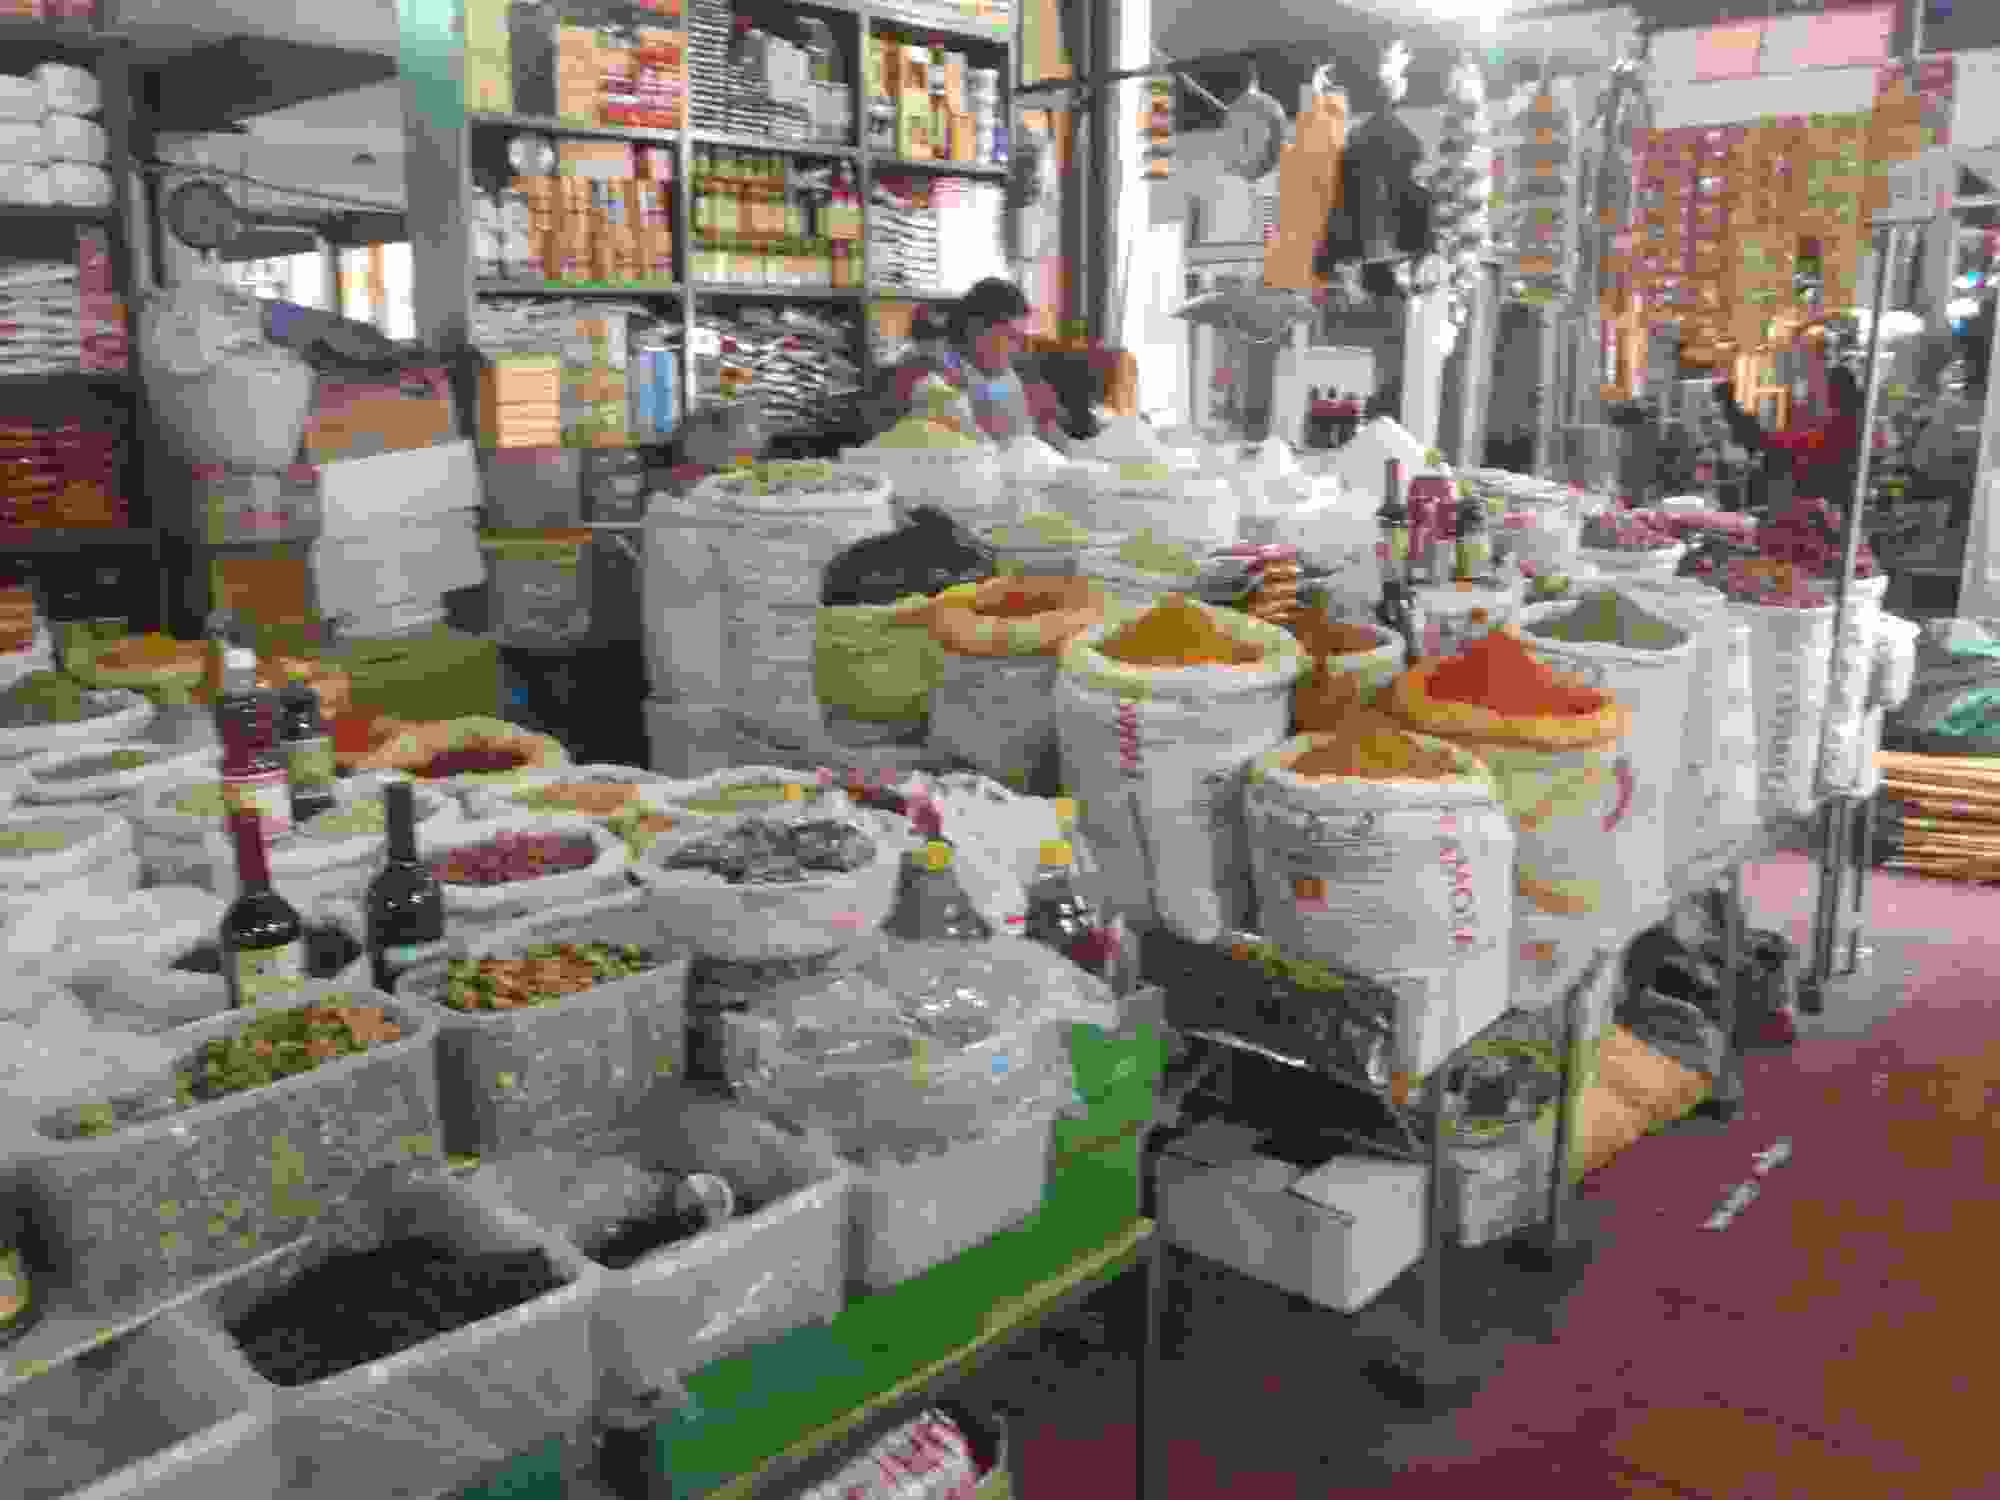
\includegraphics[width=\mywidth]{../wp-content/uploads/2015/04/wpid-wp-1429062996837.jpg} } 
 \newline
 \newline
\centerline{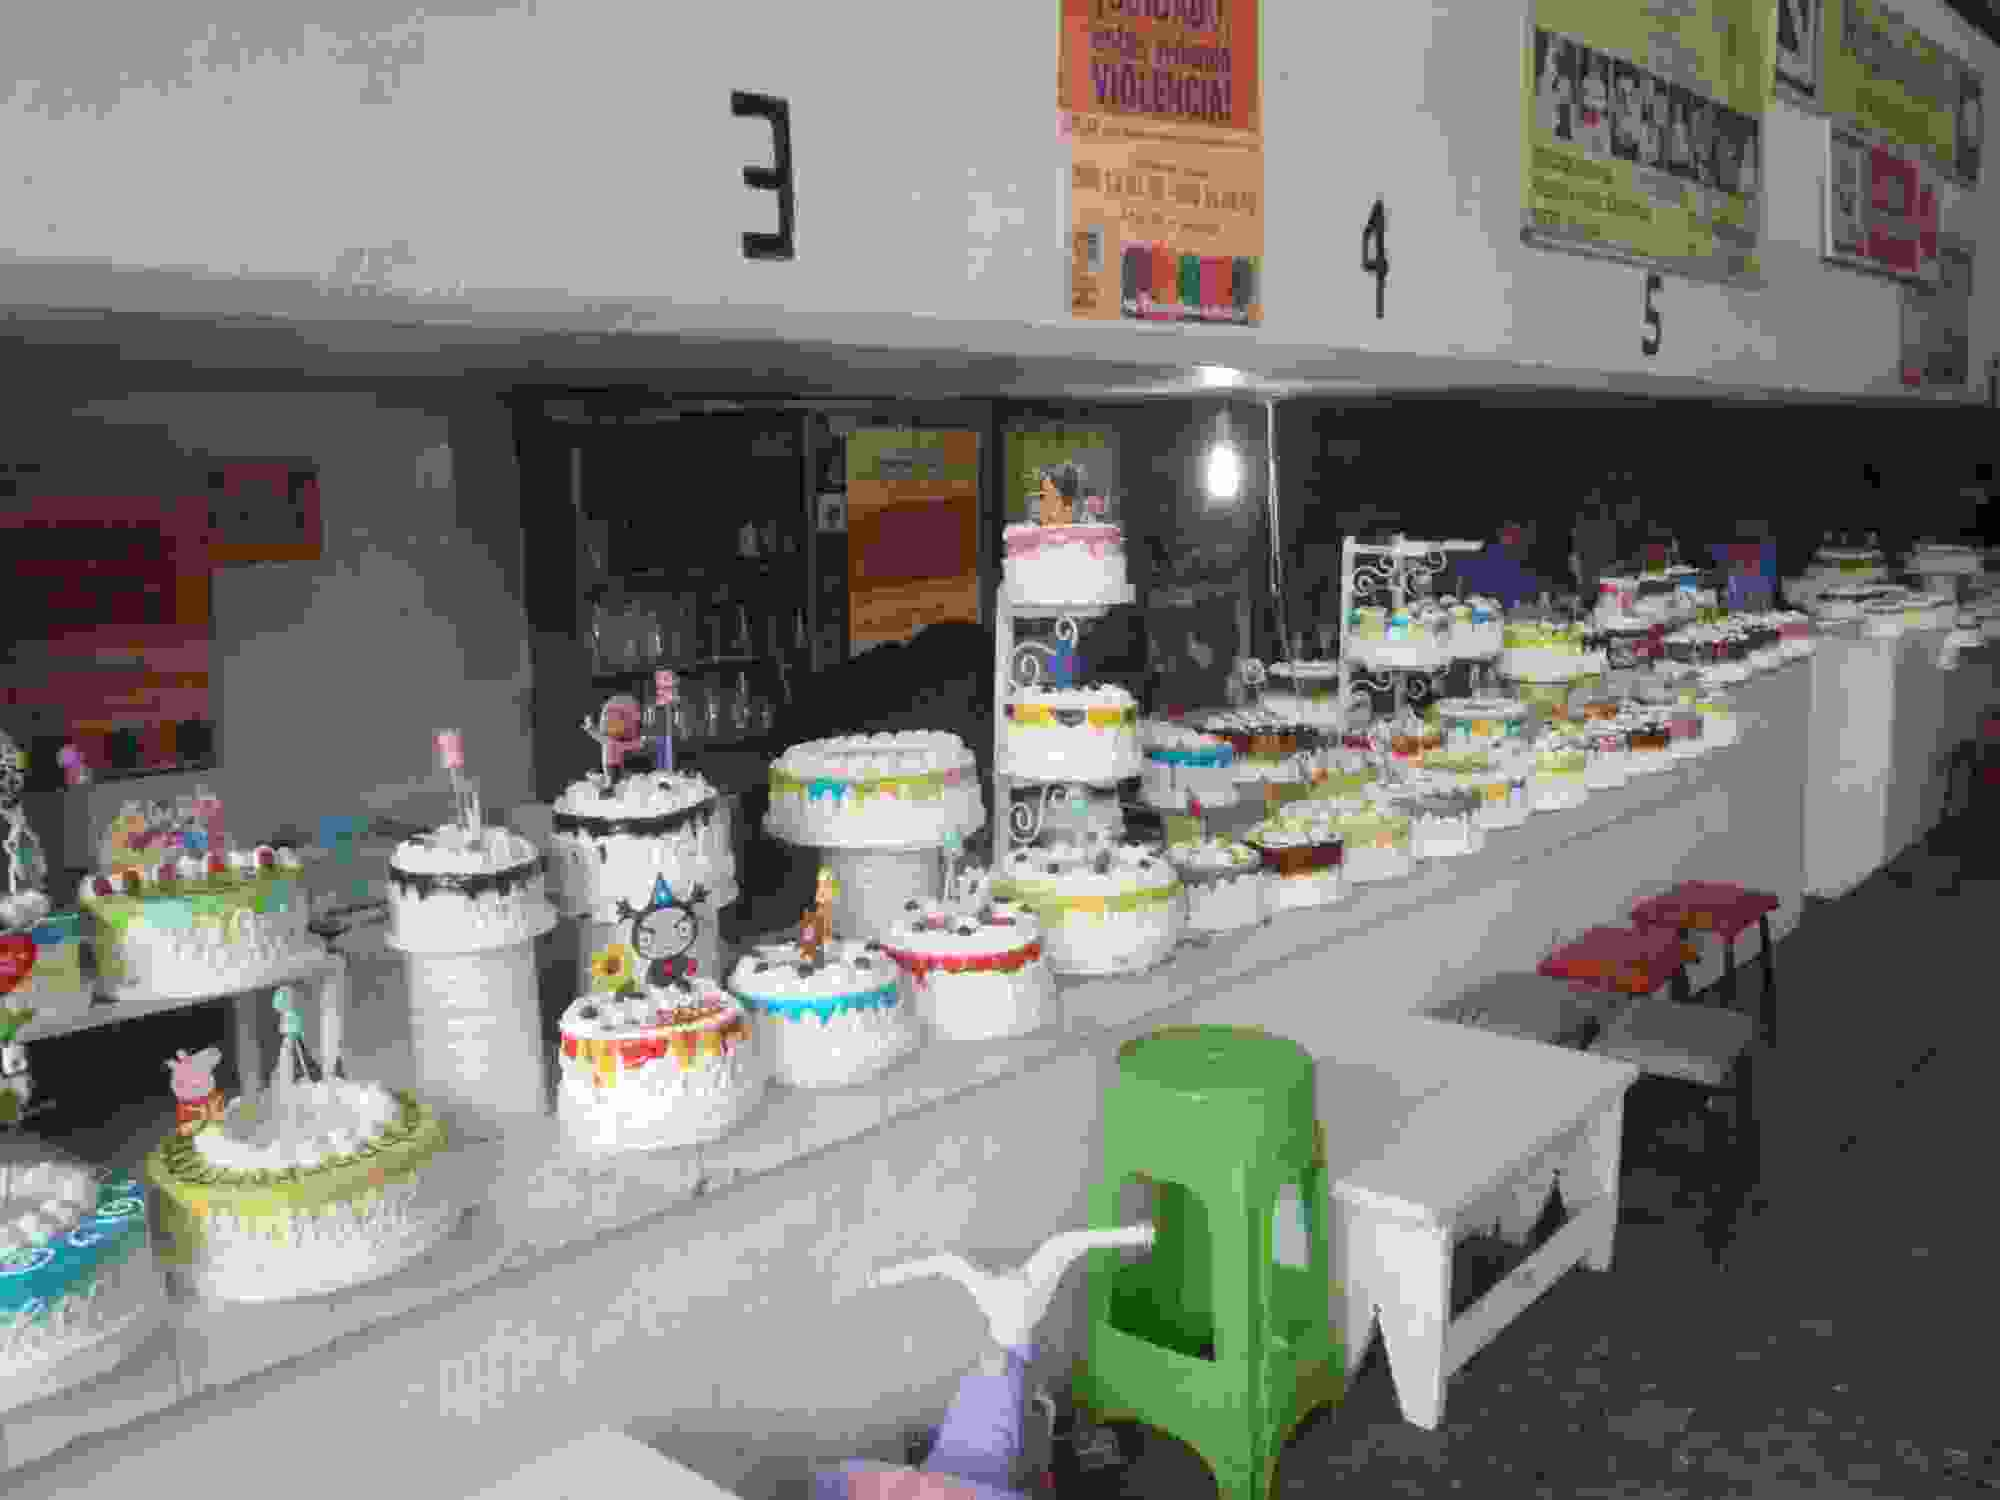
\includegraphics[width=\mywidth]{../wp-content/uploads/2015/04/wpid-wp-1429063009158.jpg} } 
 \newline
 Les stands qui servent des jus et des salades de fruits : un régal et pas cher.  \newline
 \newline
\centerline{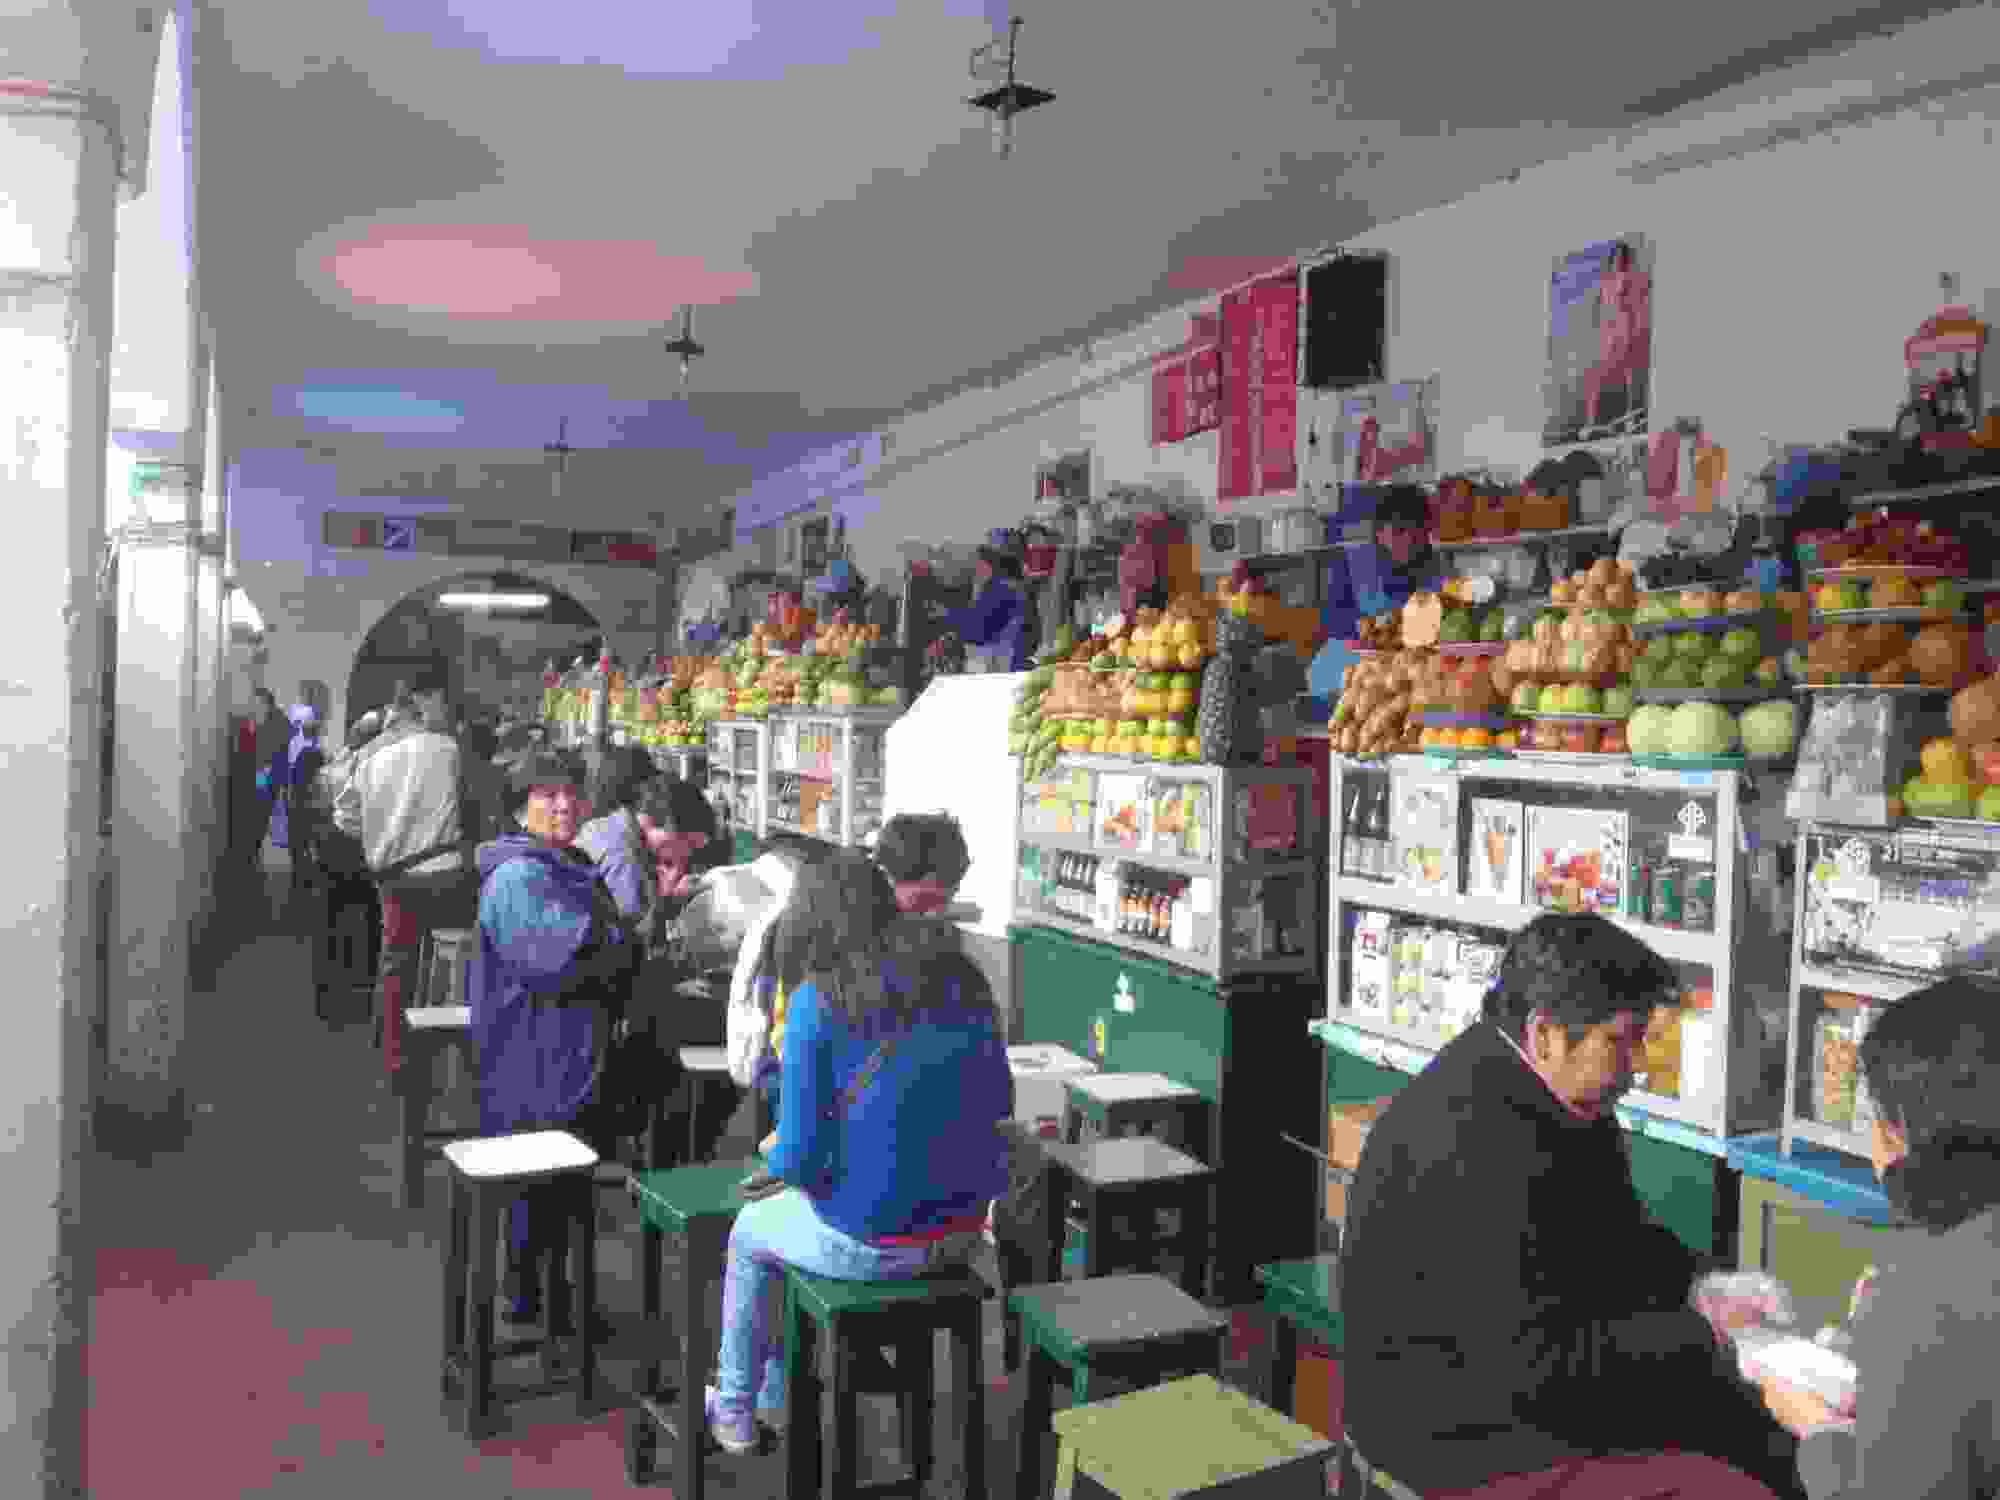
\includegraphics[width=\mywidth]{../wp-content/uploads/2015/04/wpid-wp-1429063121415.jpg} } 
 \newline
 \newline
\centerline{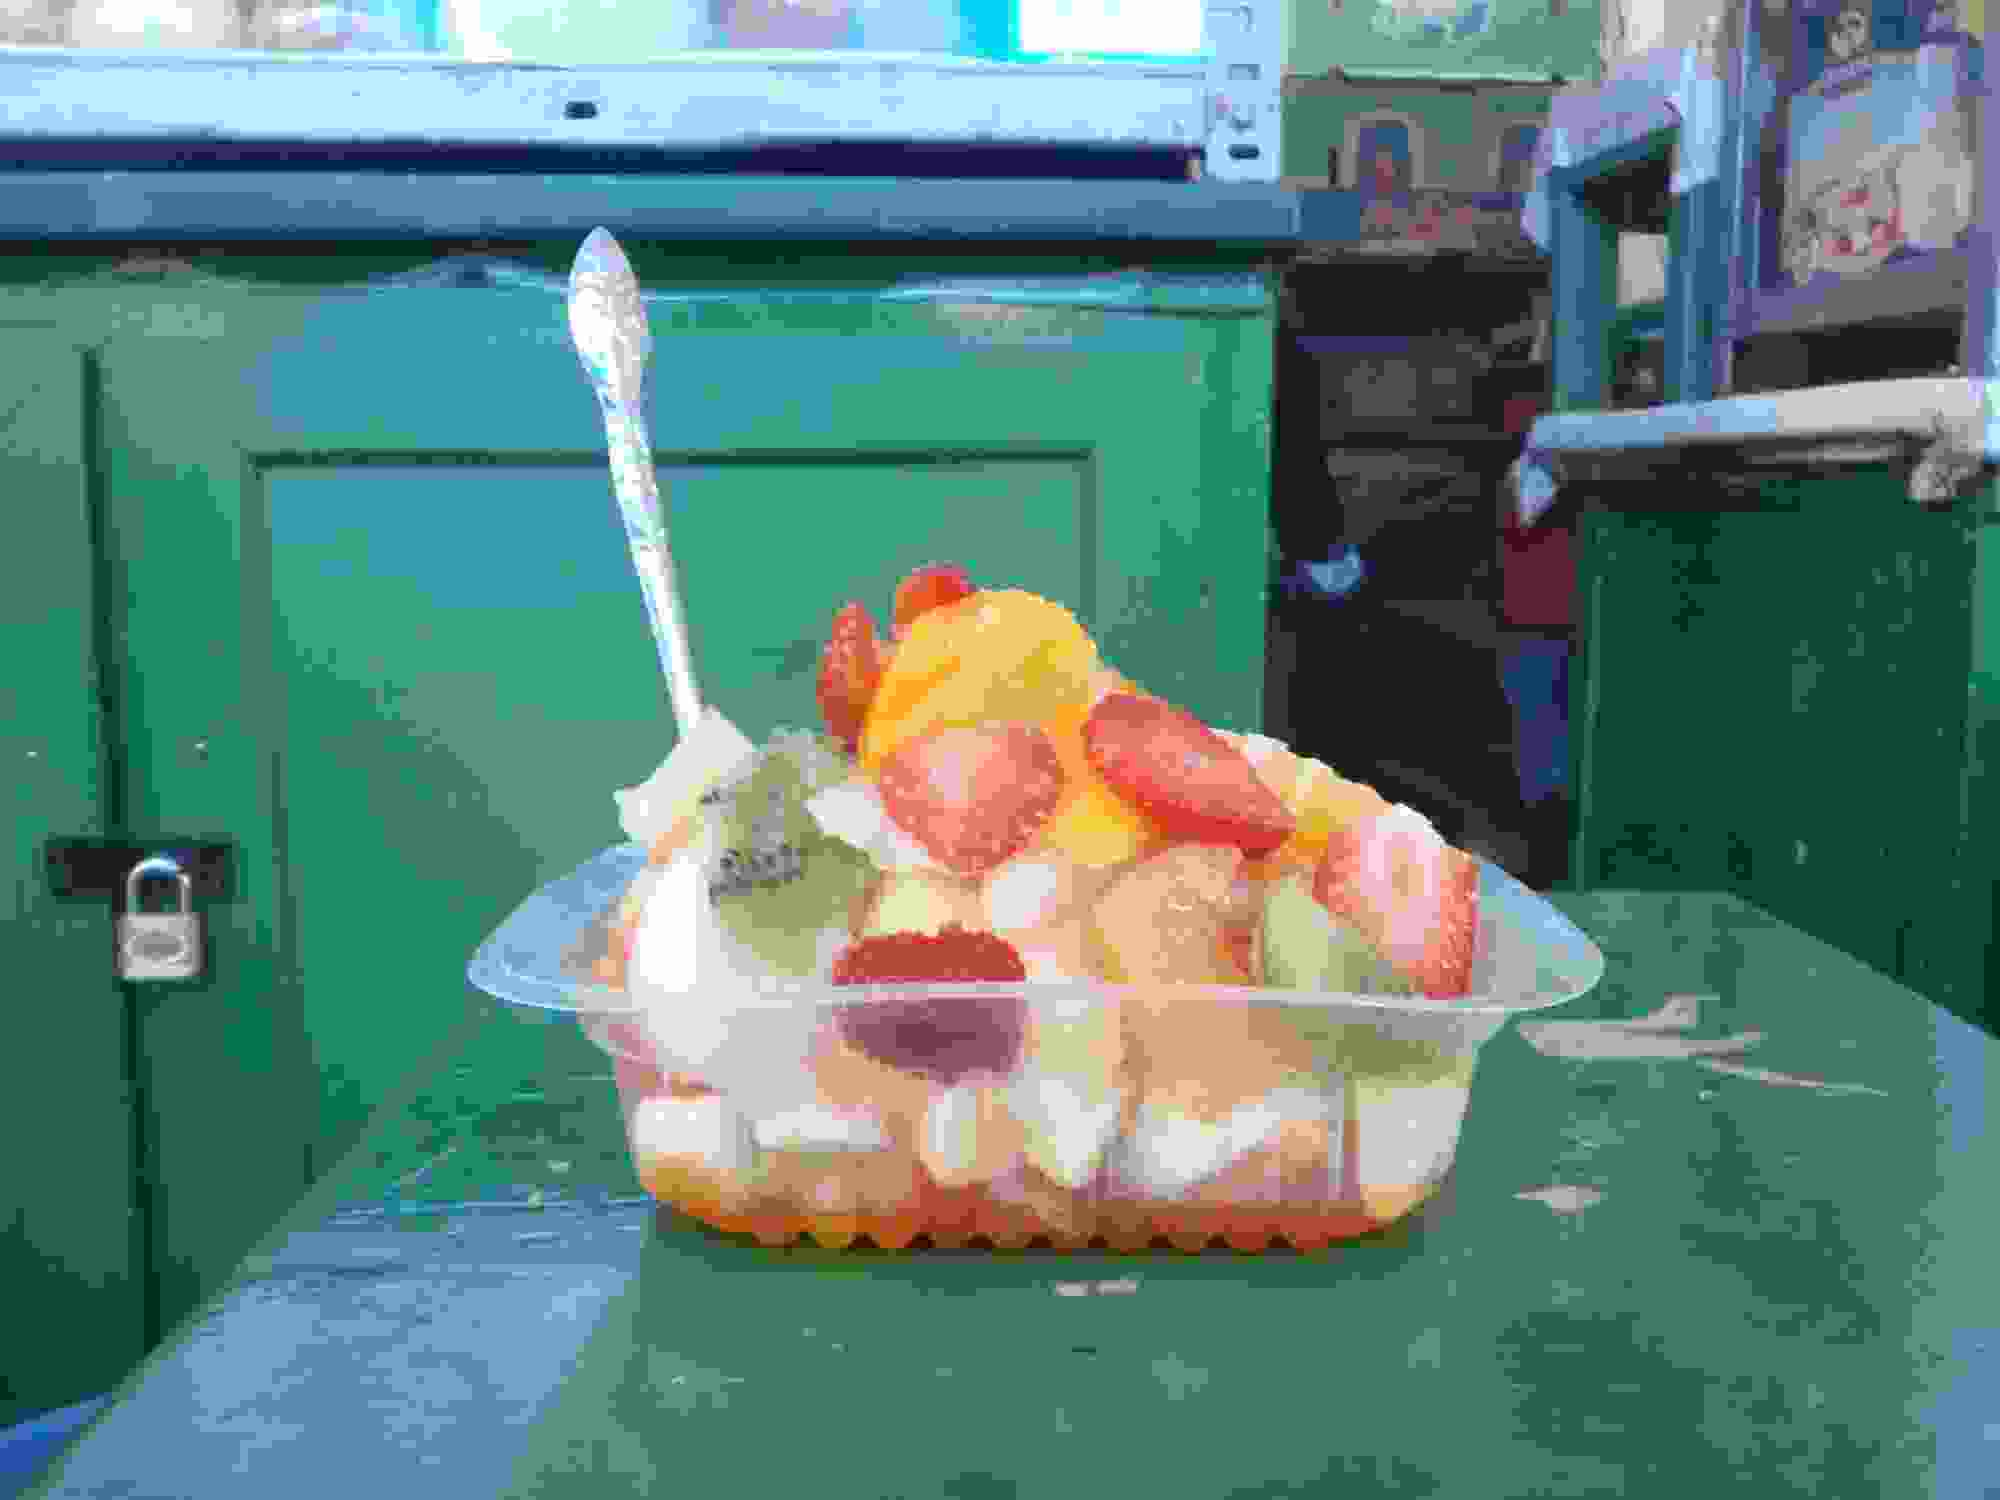
\includegraphics[width=\mywidth]{../wp-content/uploads/2015/04/wpid-wp-1429063146866.jpg} } 
 \newline
 La Recoleta, un beau point de vue sur la ville \newline
 \newline
\centerline{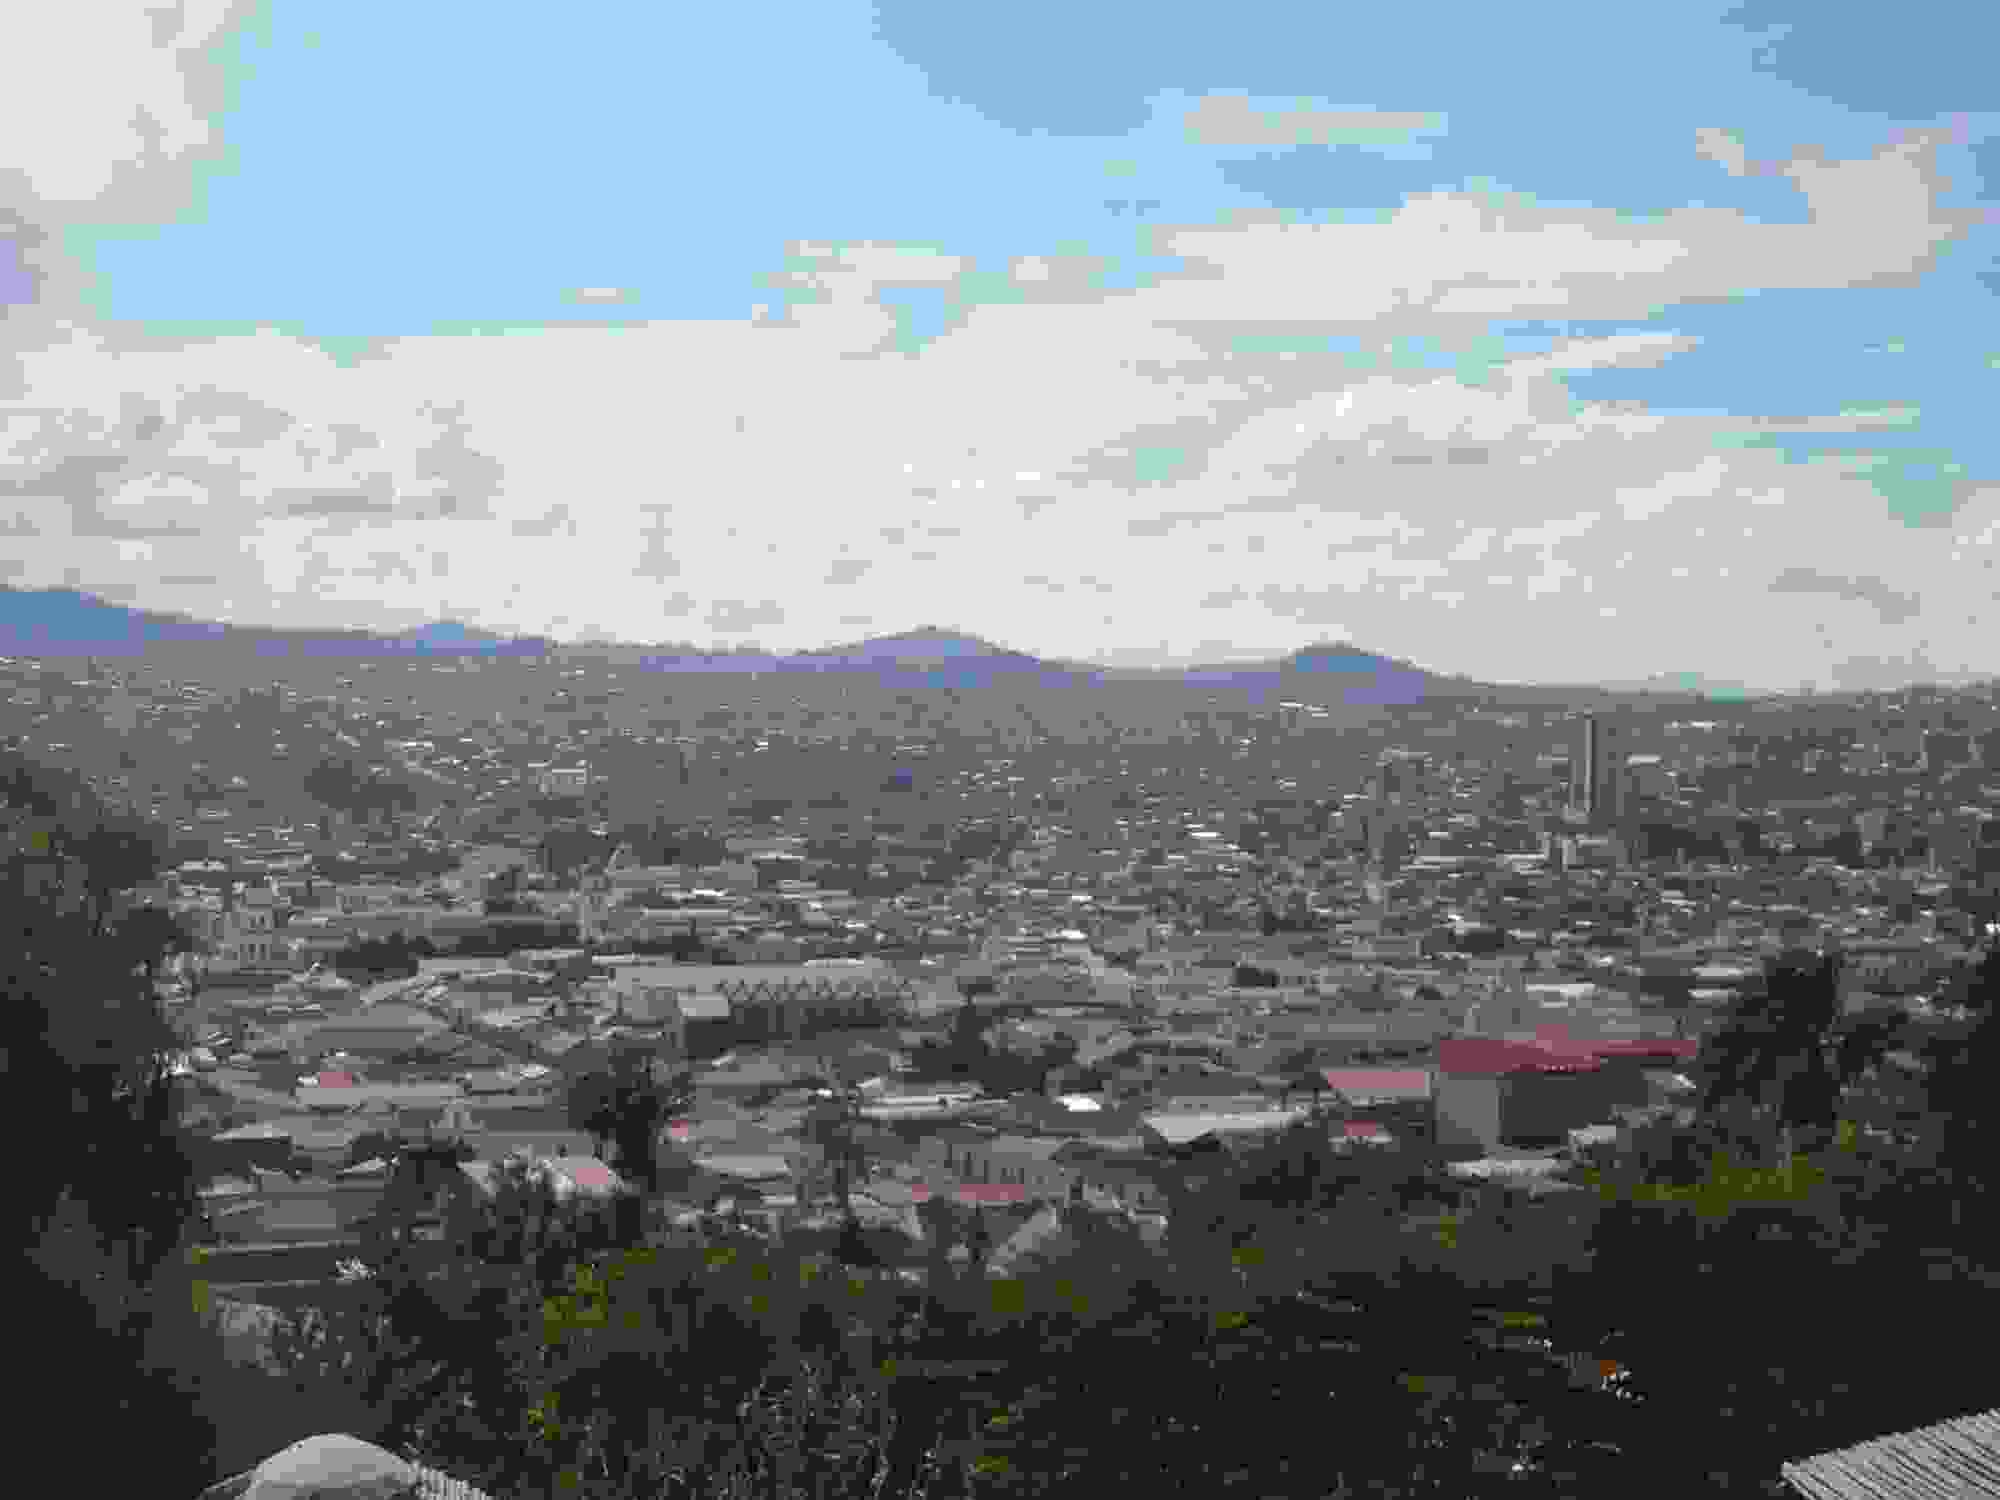
\includegraphics[width=\mywidth]{../wp-content/uploads/2015/04/wpid-wp-1429063611807.jpg} } 
 \newline
 Le parc Bolivar et sa mini tour Eiffel \newline
 \newline
\centerline{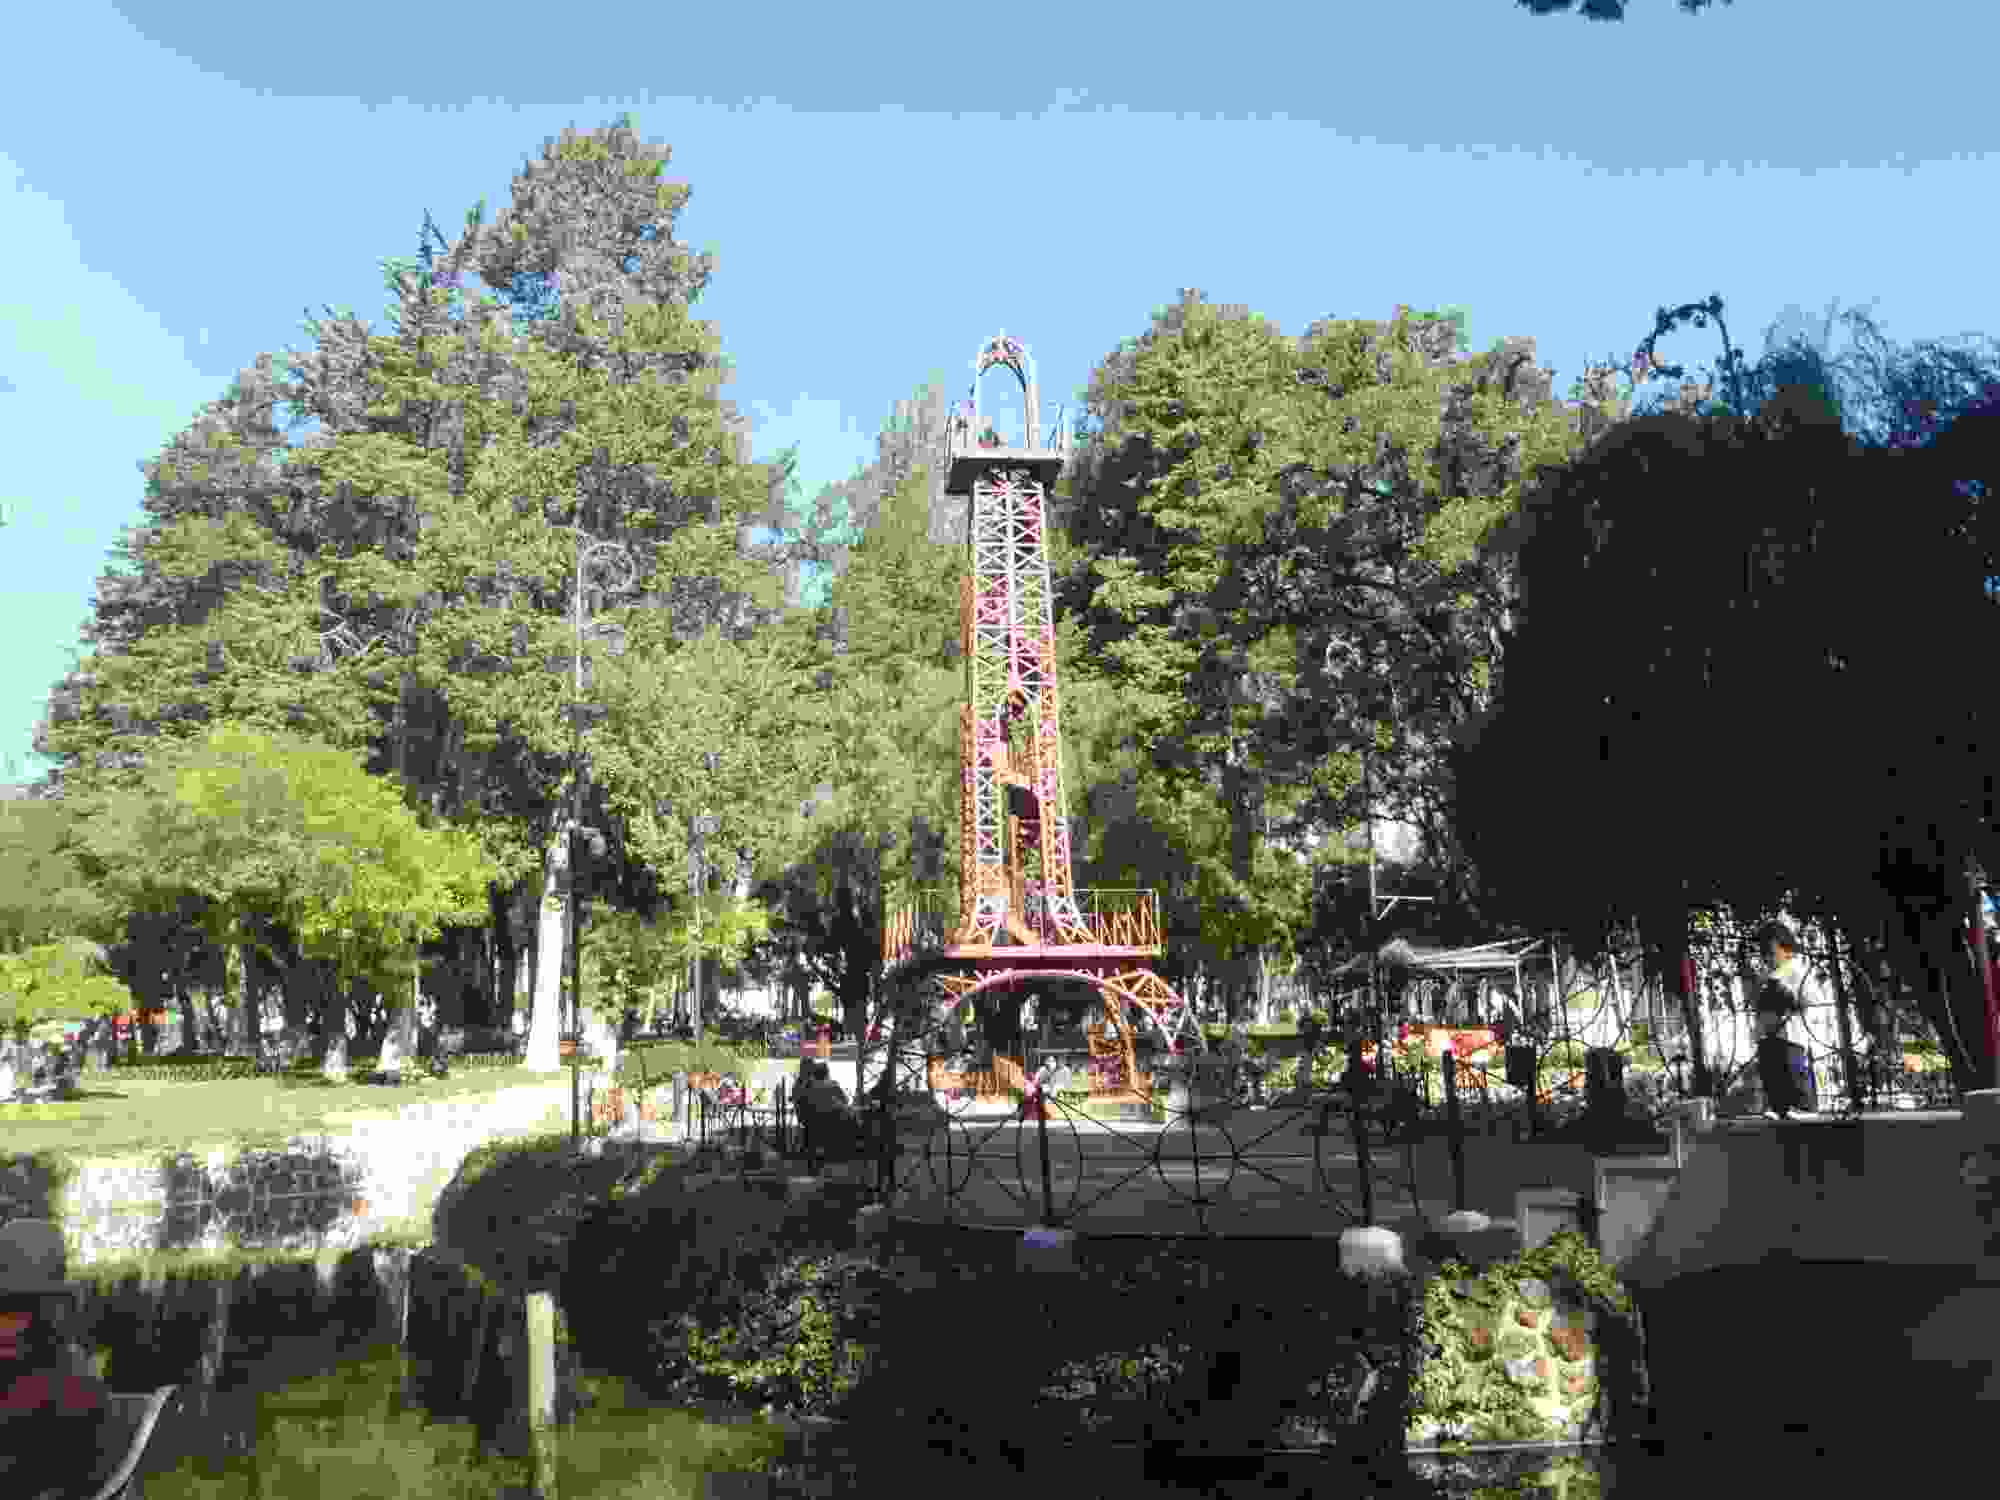
\includegraphics[width=\mywidth]{../wp-content/uploads/2015/04/wpid-wp-1429063685140.jpg} } 
 \newline
 Le Cementario General \newline
 \newline
\centerline{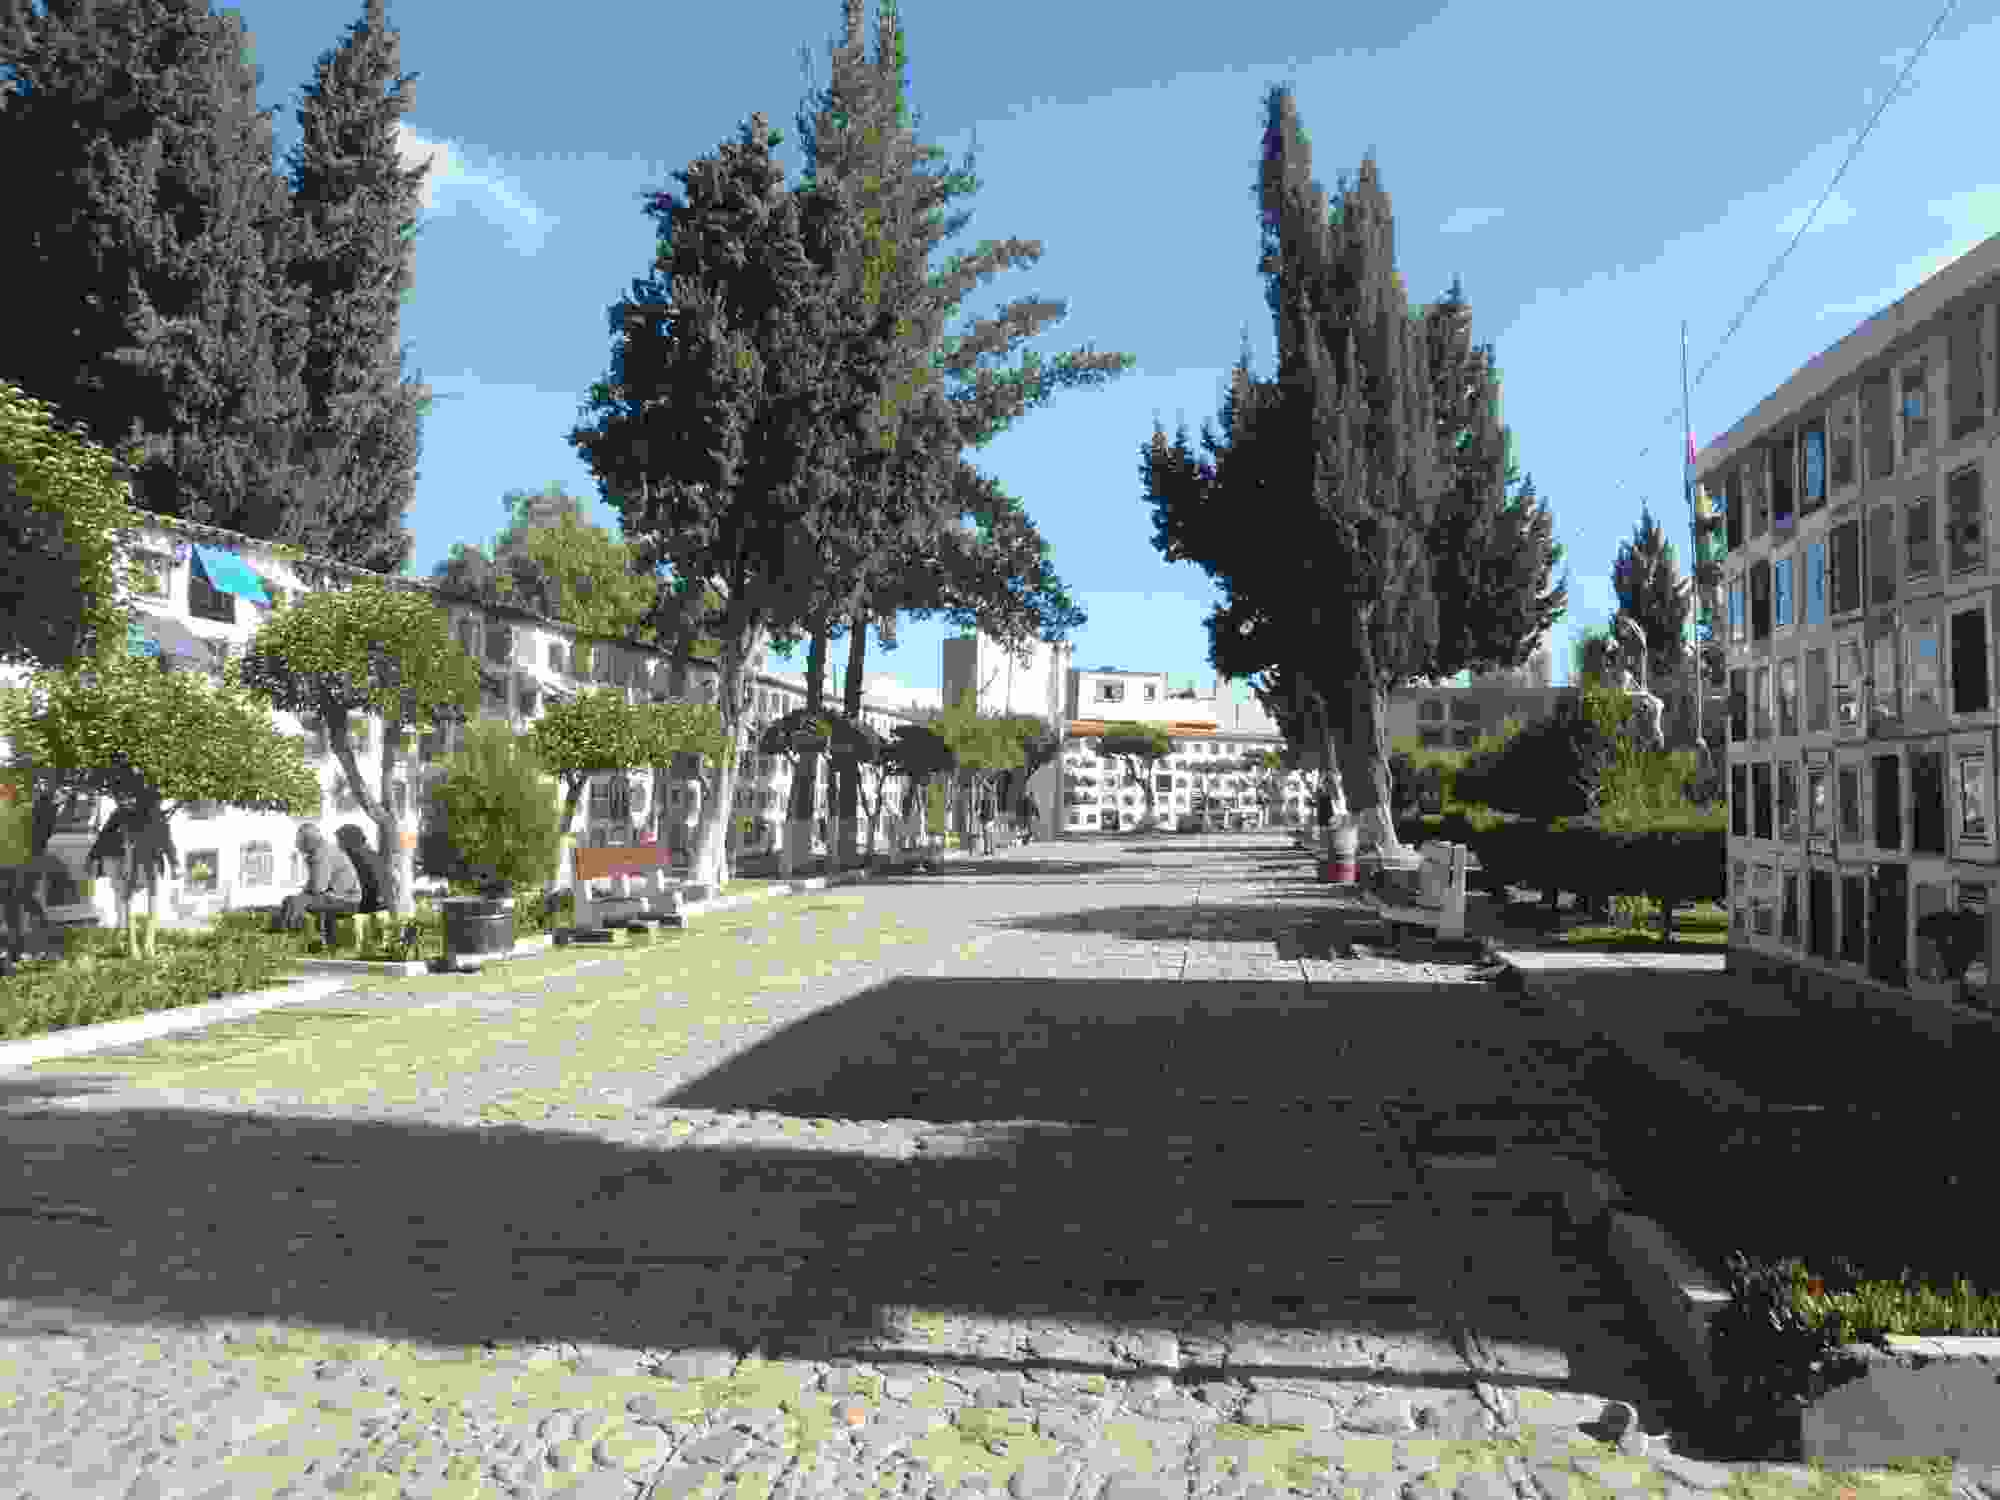
\includegraphics[width=\mywidth]{../wp-content/uploads/2015/04/wpid-wp-1429063755883.jpg} } 
 \newline
 \newline
\centerline{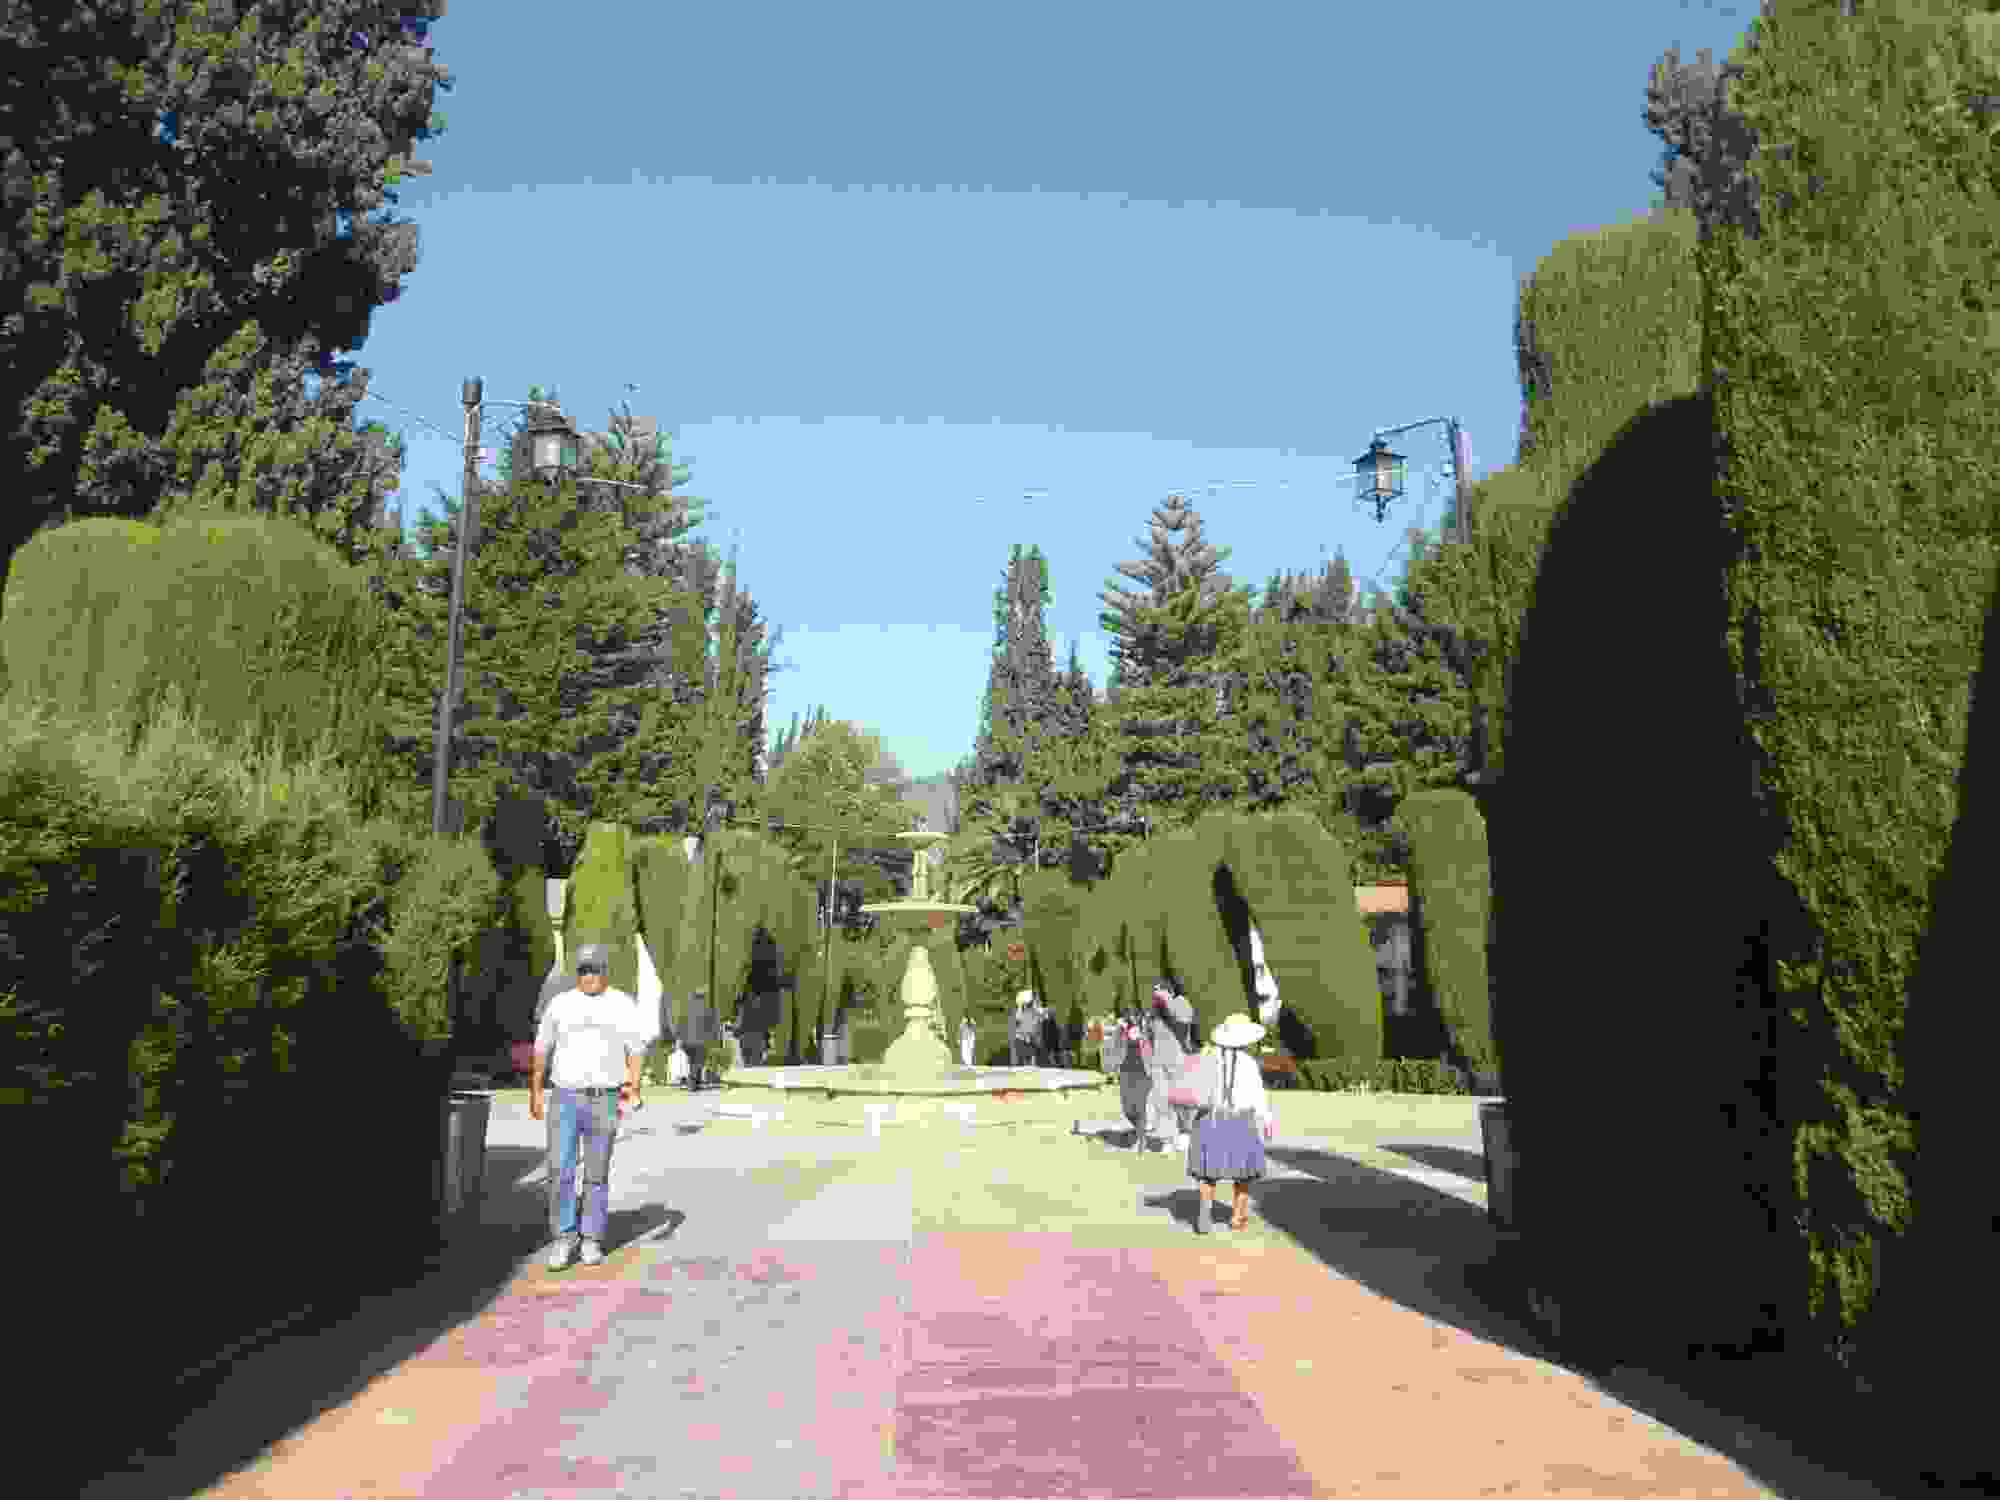
\includegraphics[width=\mywidth]{../wp-content/uploads/2015/04/wpid-wp-1429063782119.jpg} } 
 \newline
 Grâce à Couchsurfing j'ai rencontré Omar un étudiant bolivien. Avec 2 de ses amis, on a visité le parc des dinosaures : \newline
 \newline
\centerline{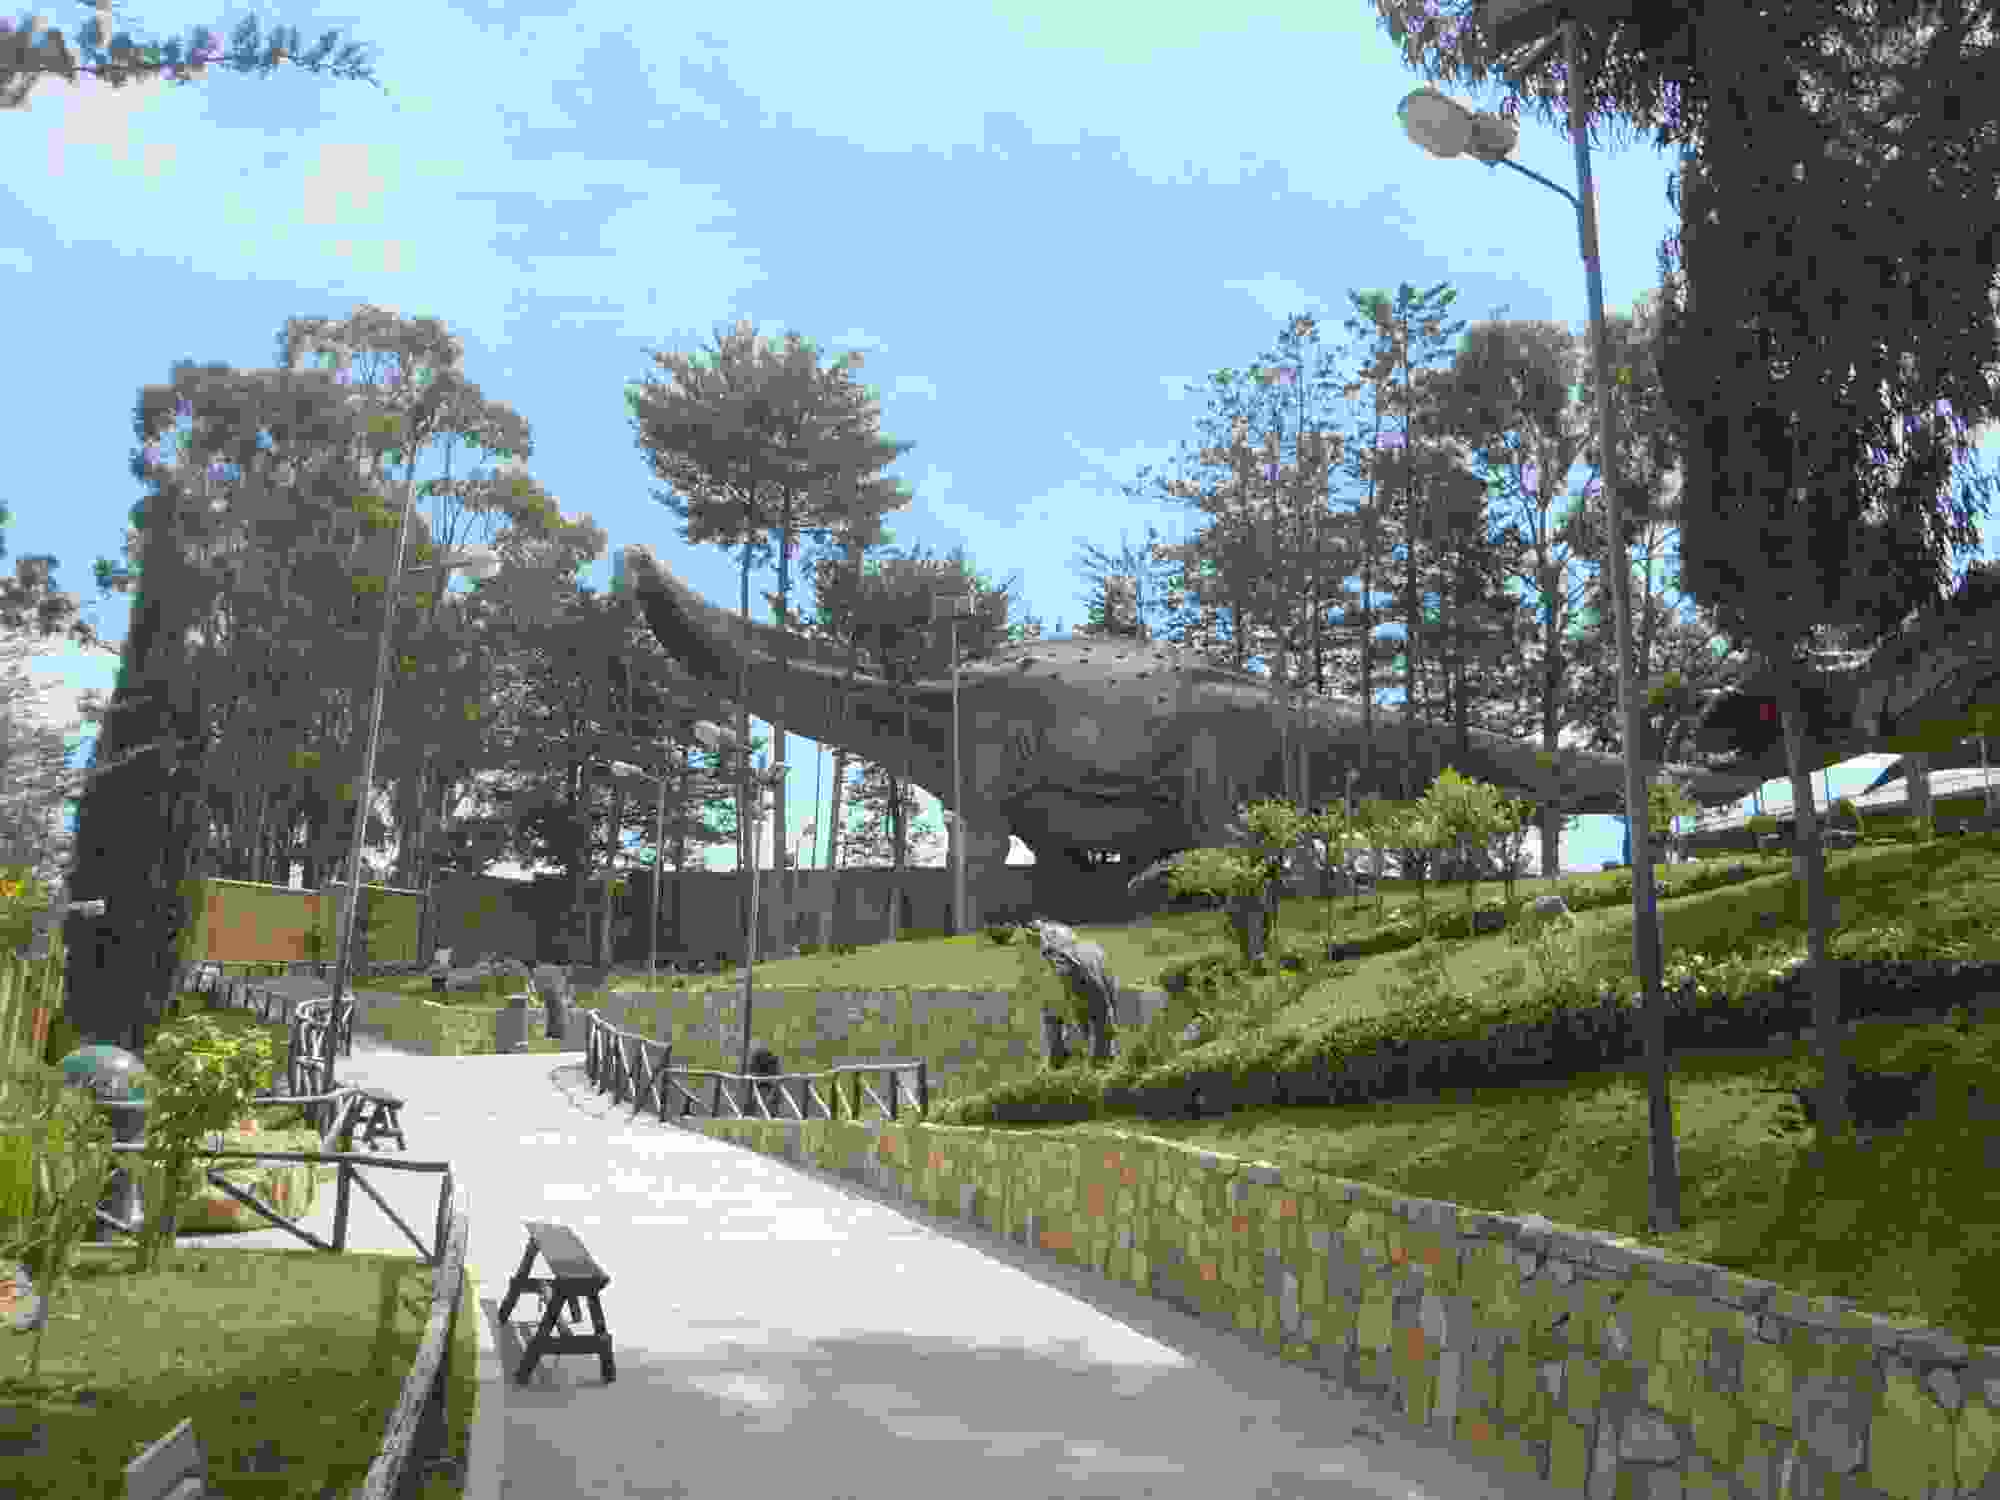
\includegraphics[width=\mywidth]{../wp-content/uploads/2015/04/wpid-wp-1429064168634.jpg} } 
 \newline
 \newline
\centerline{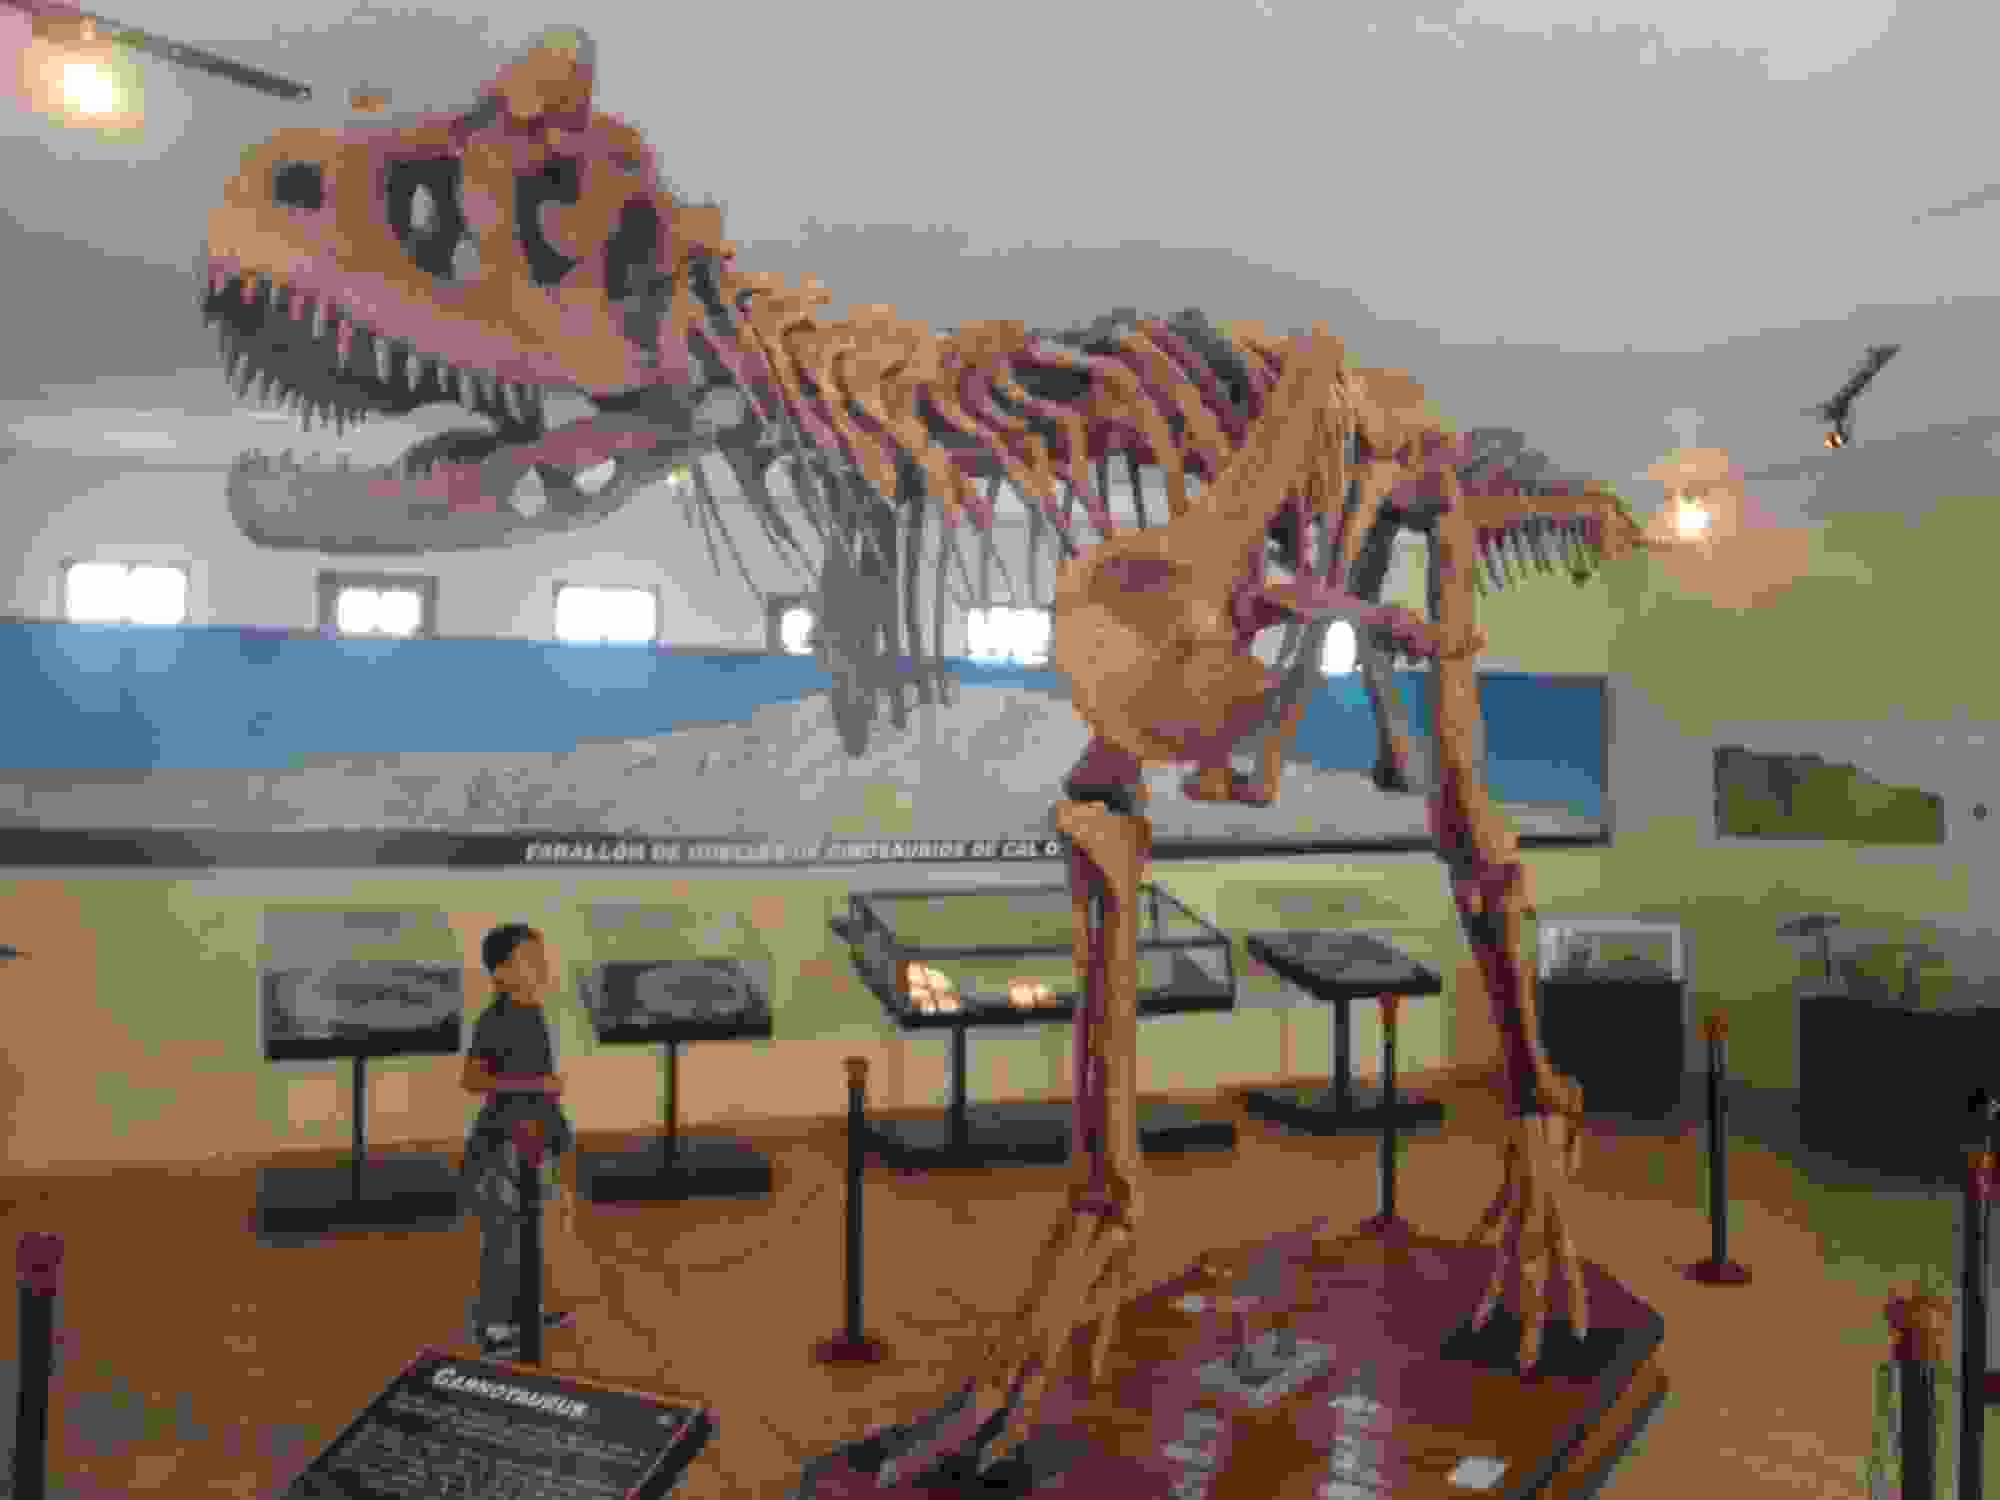
\includegraphics[width=\mywidth]{../wp-content/uploads/2015/04/wpid-wp-1429064265257.jpg} } 
 \newline
 La tectonique des plaques a fait passer cette immense falaise de l'horizontale à la verticale. Puis l'exploitation du site pour la fabrication de ciment a permis de découvrir des centaines d'empreintes de dinosaures.  \newline
 \newline
\centerline{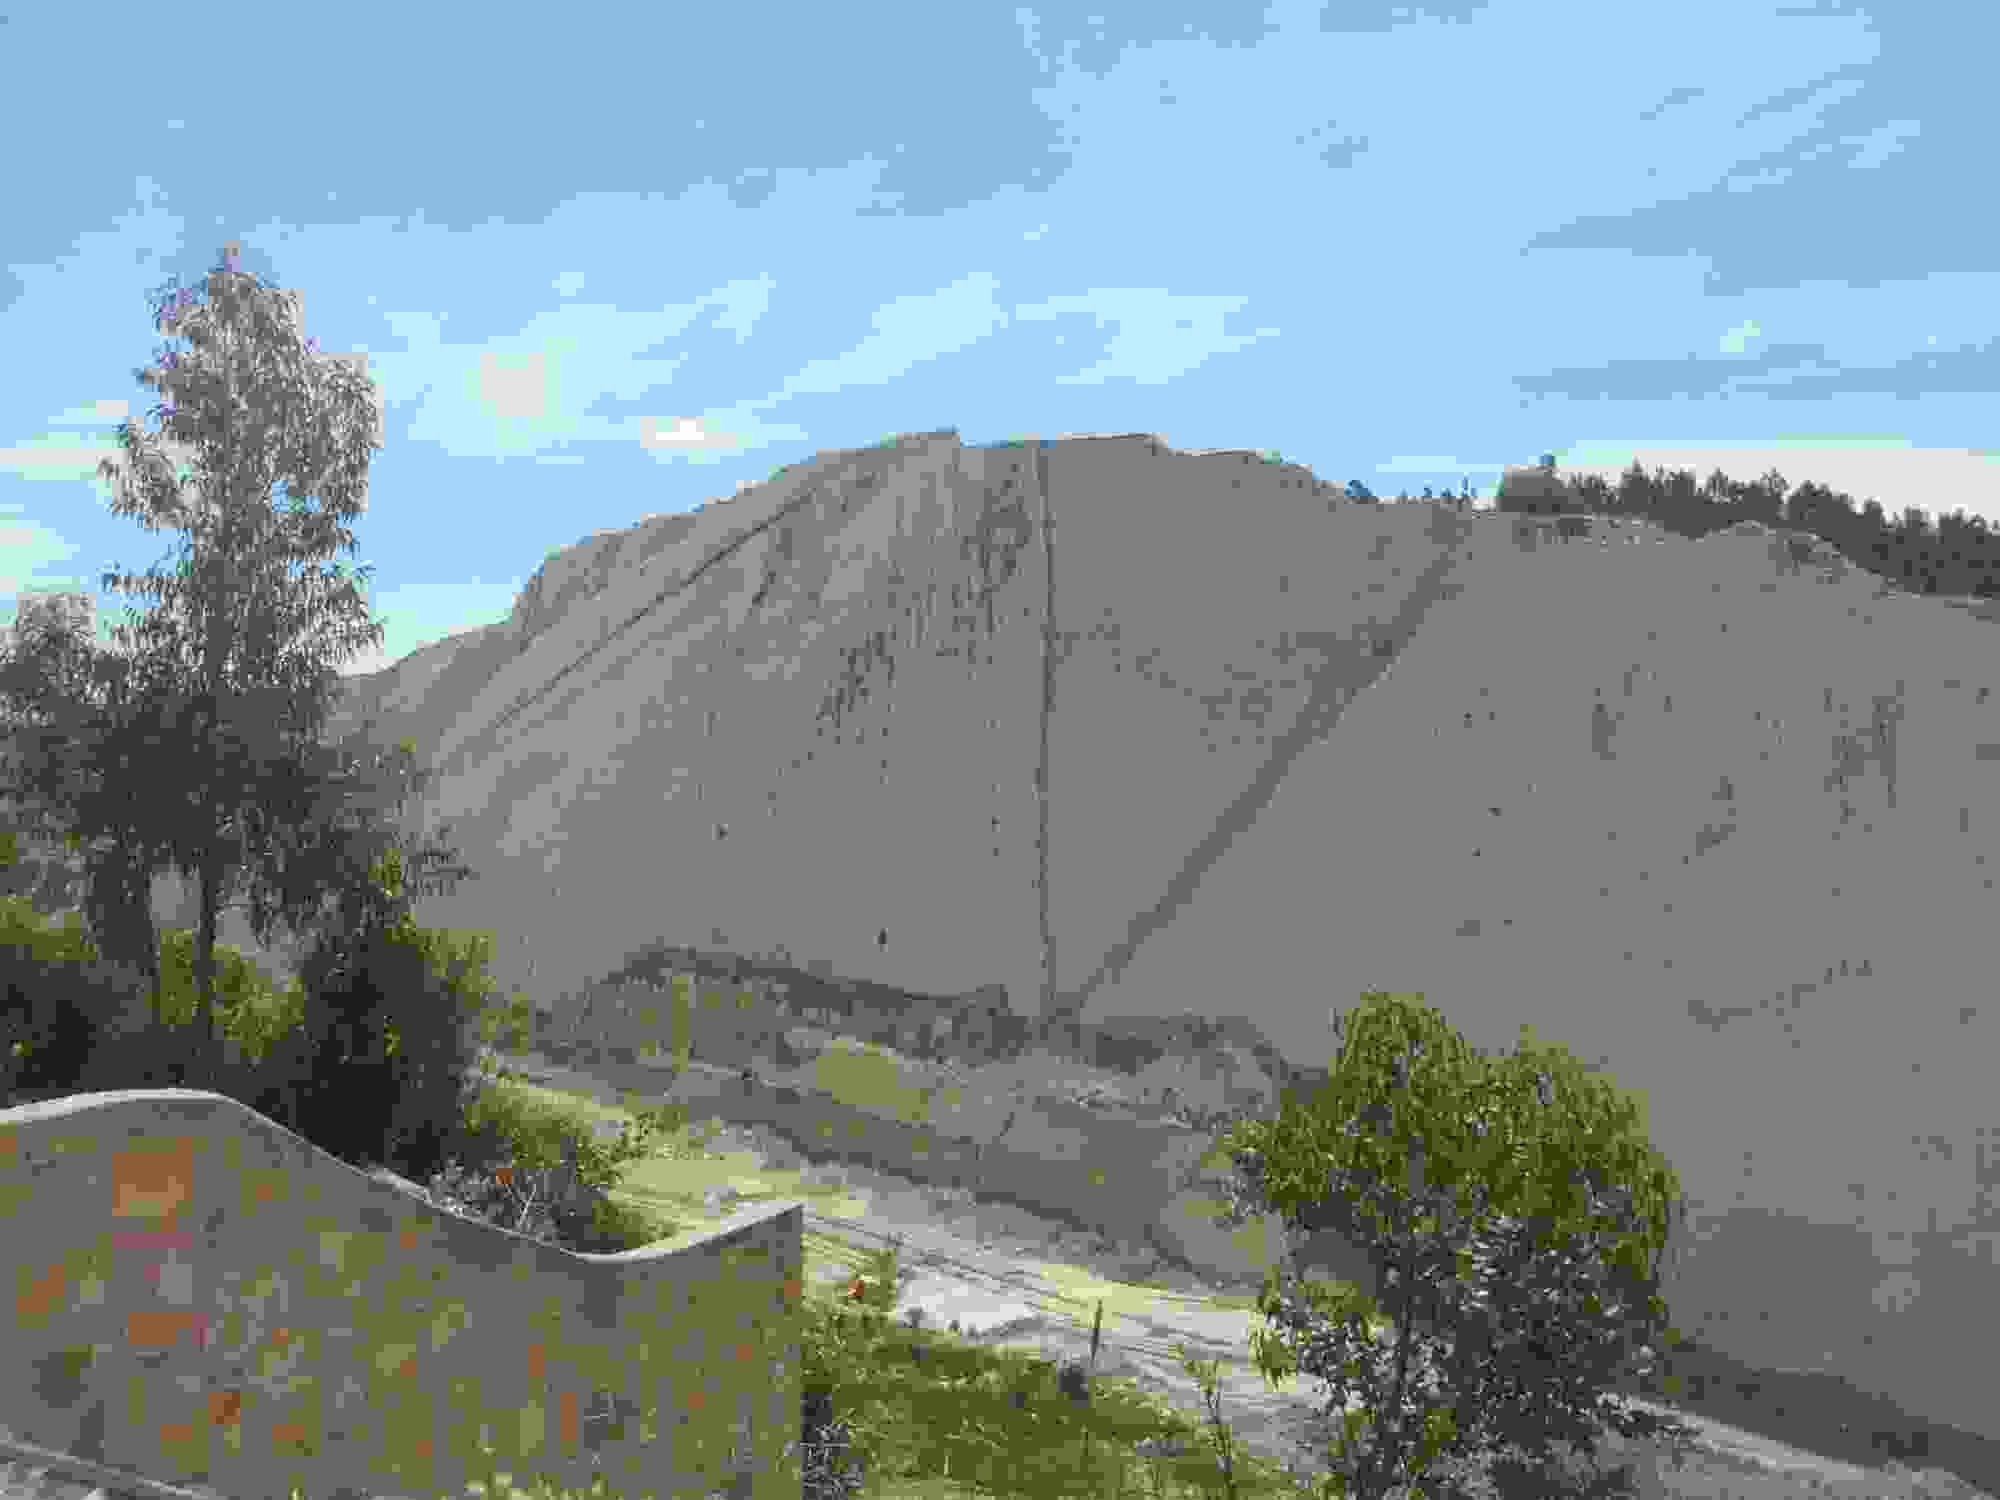
\includegraphics[width=\mywidth]{../wp-content/uploads/2015/04/wpid-wp-1429064563362.jpg} } 
 \newline
 \newline
\centerline{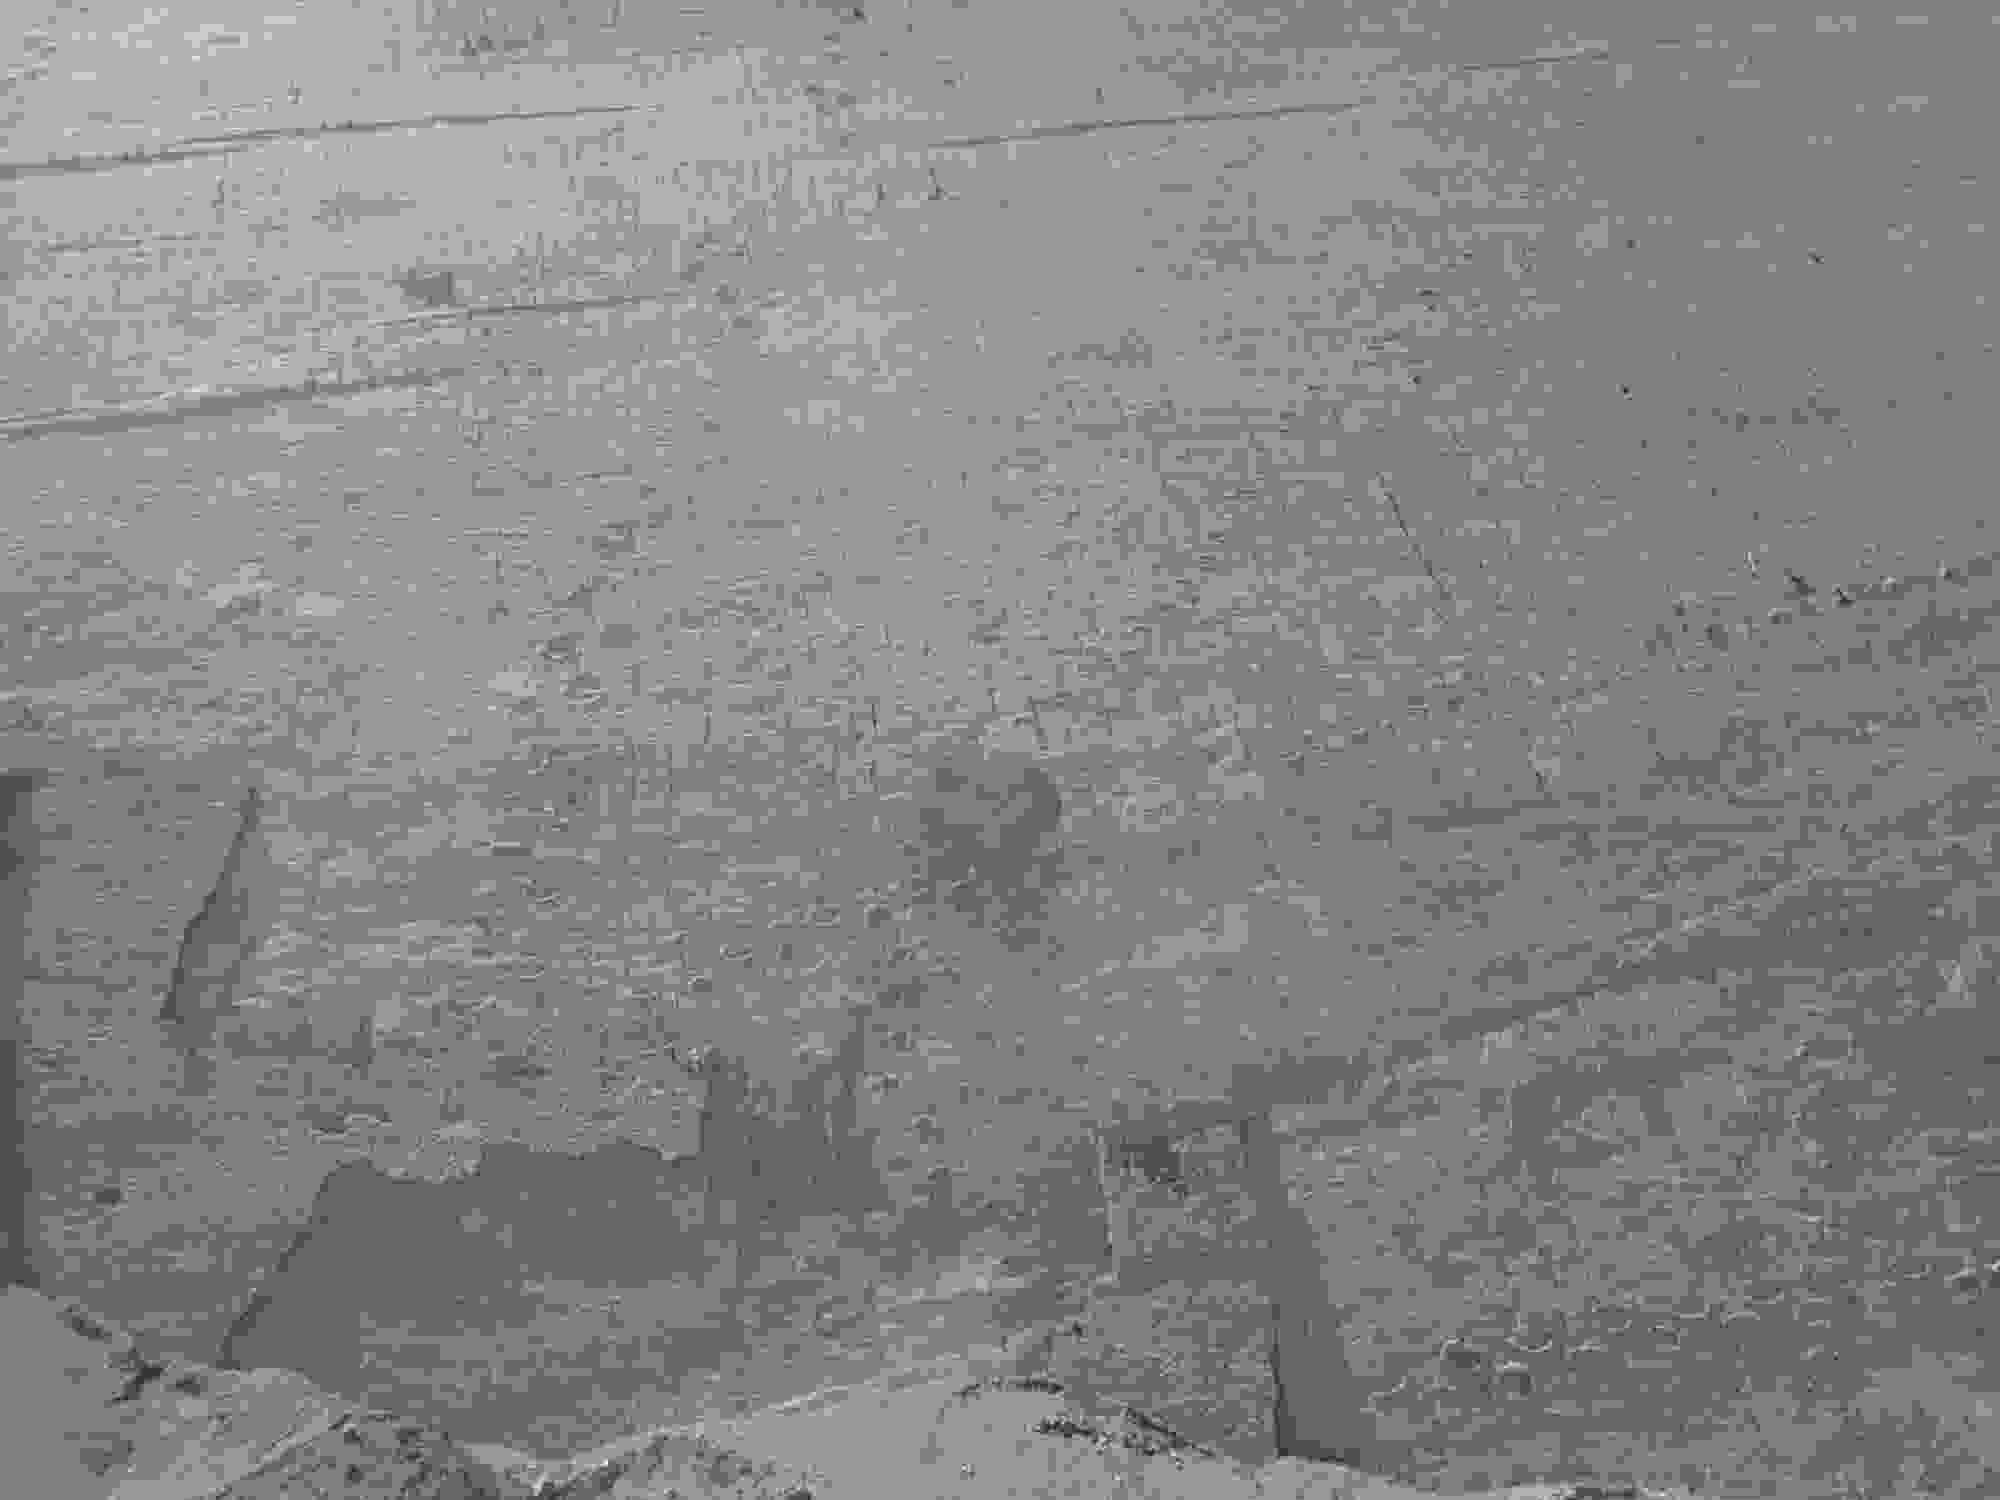
\includegraphics[width=\mywidth]{../wp-content/uploads/2015/04/wpid-wp-1429064631714.jpg} } 
 \newline
 \newline
\centerline{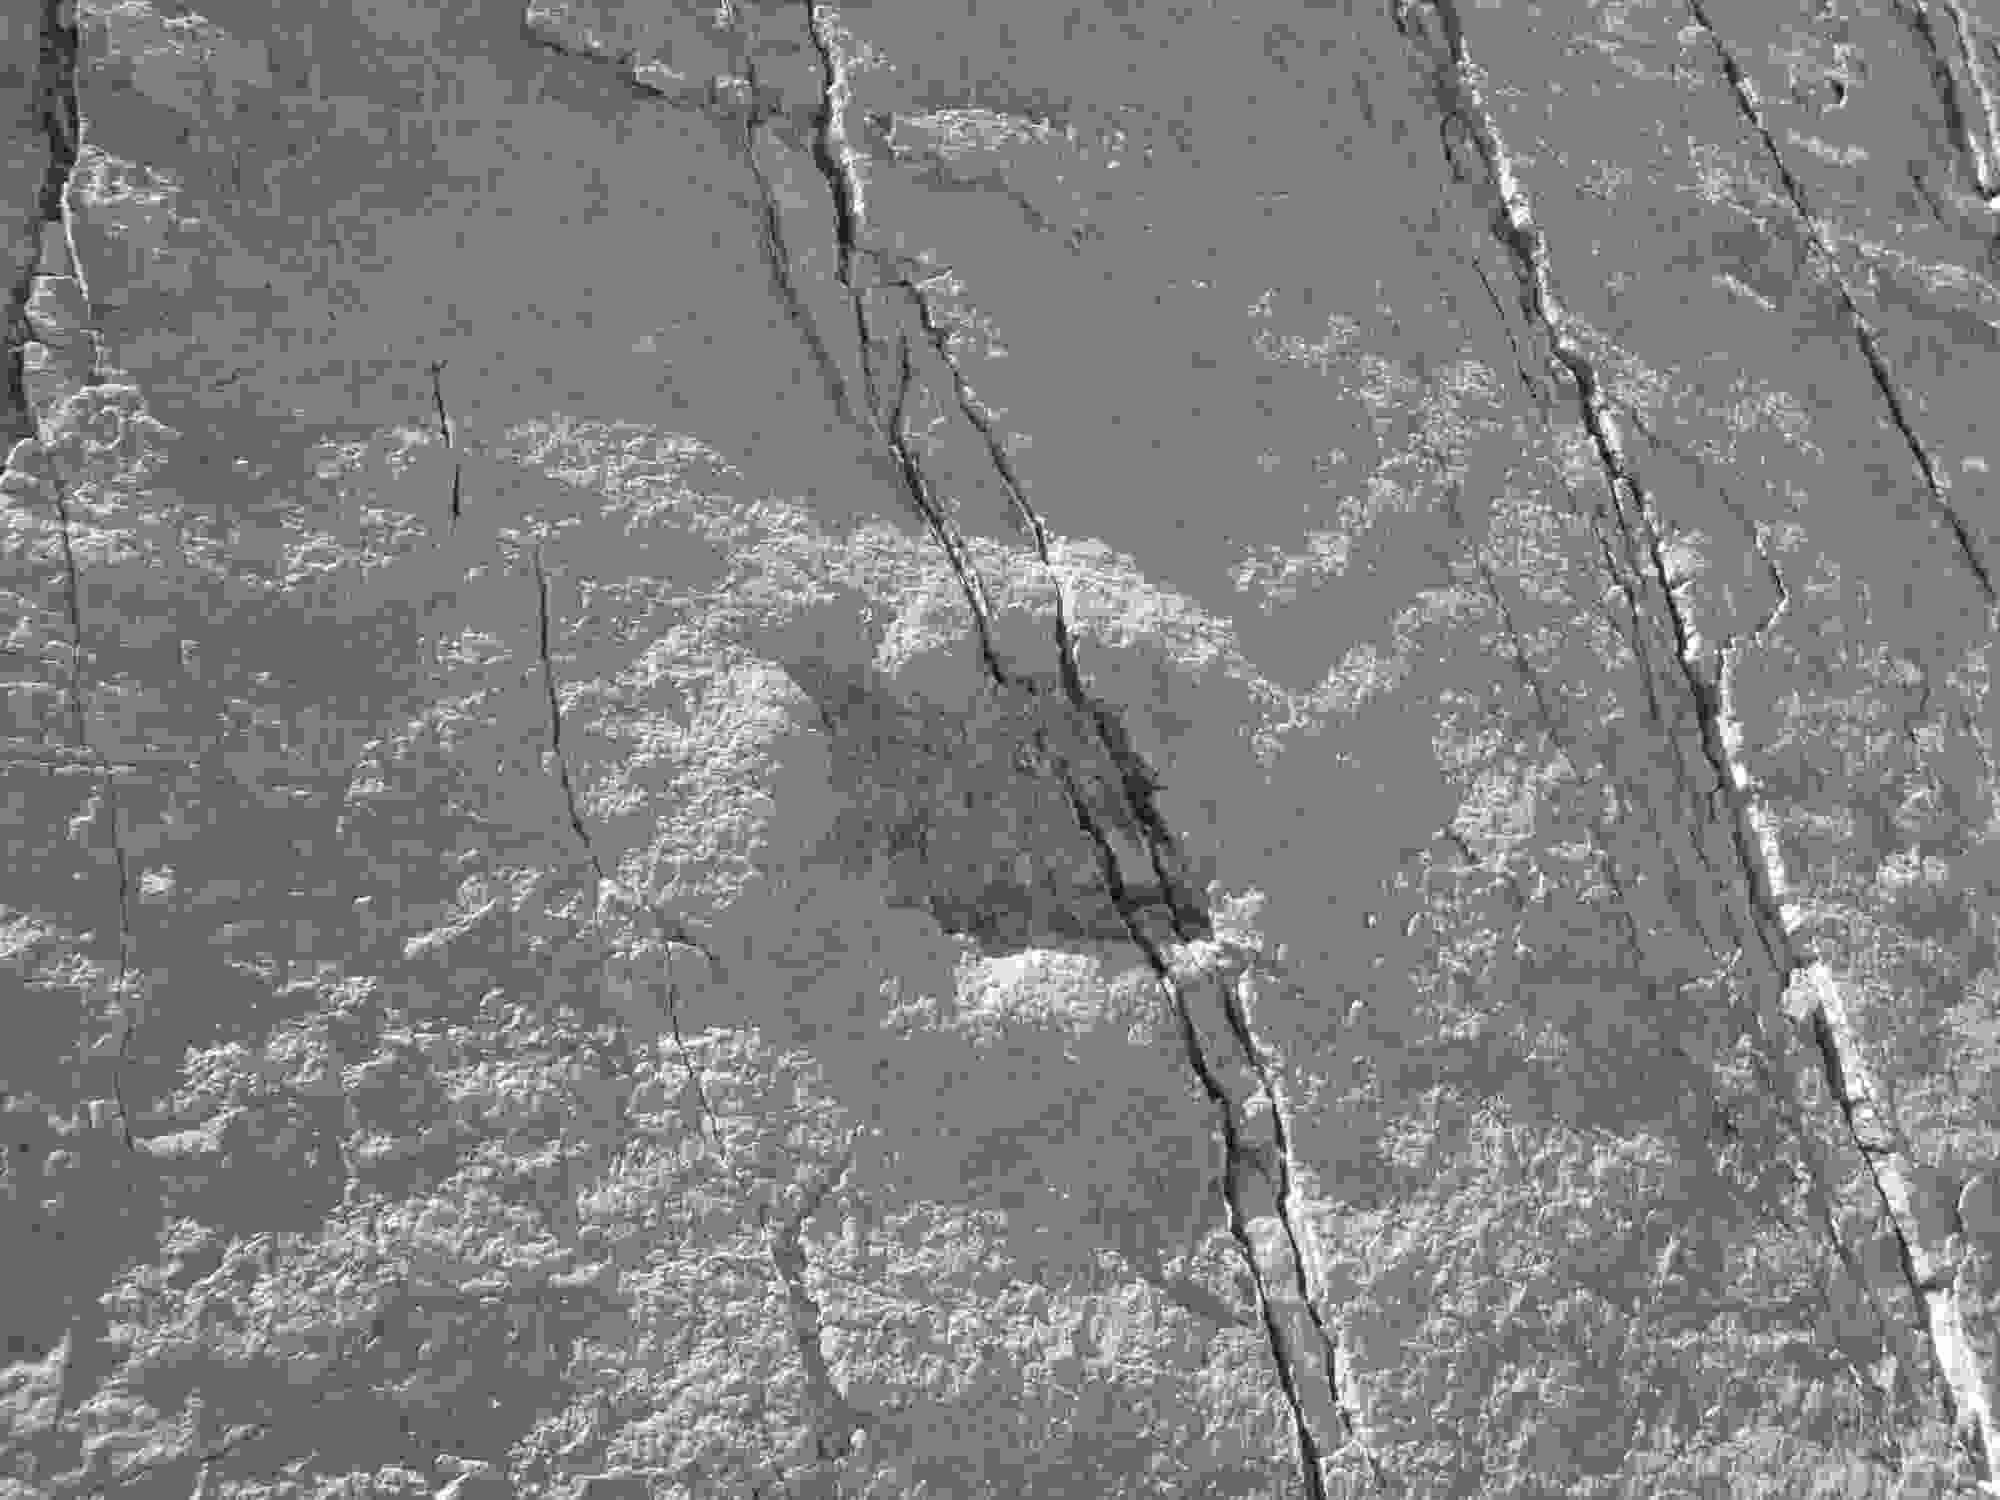
\includegraphics[width=\mywidth]{../wp-content/uploads/2015/04/wpid-wp-1429064717017.jpg} } 
 \newline
 \newline
\centerline{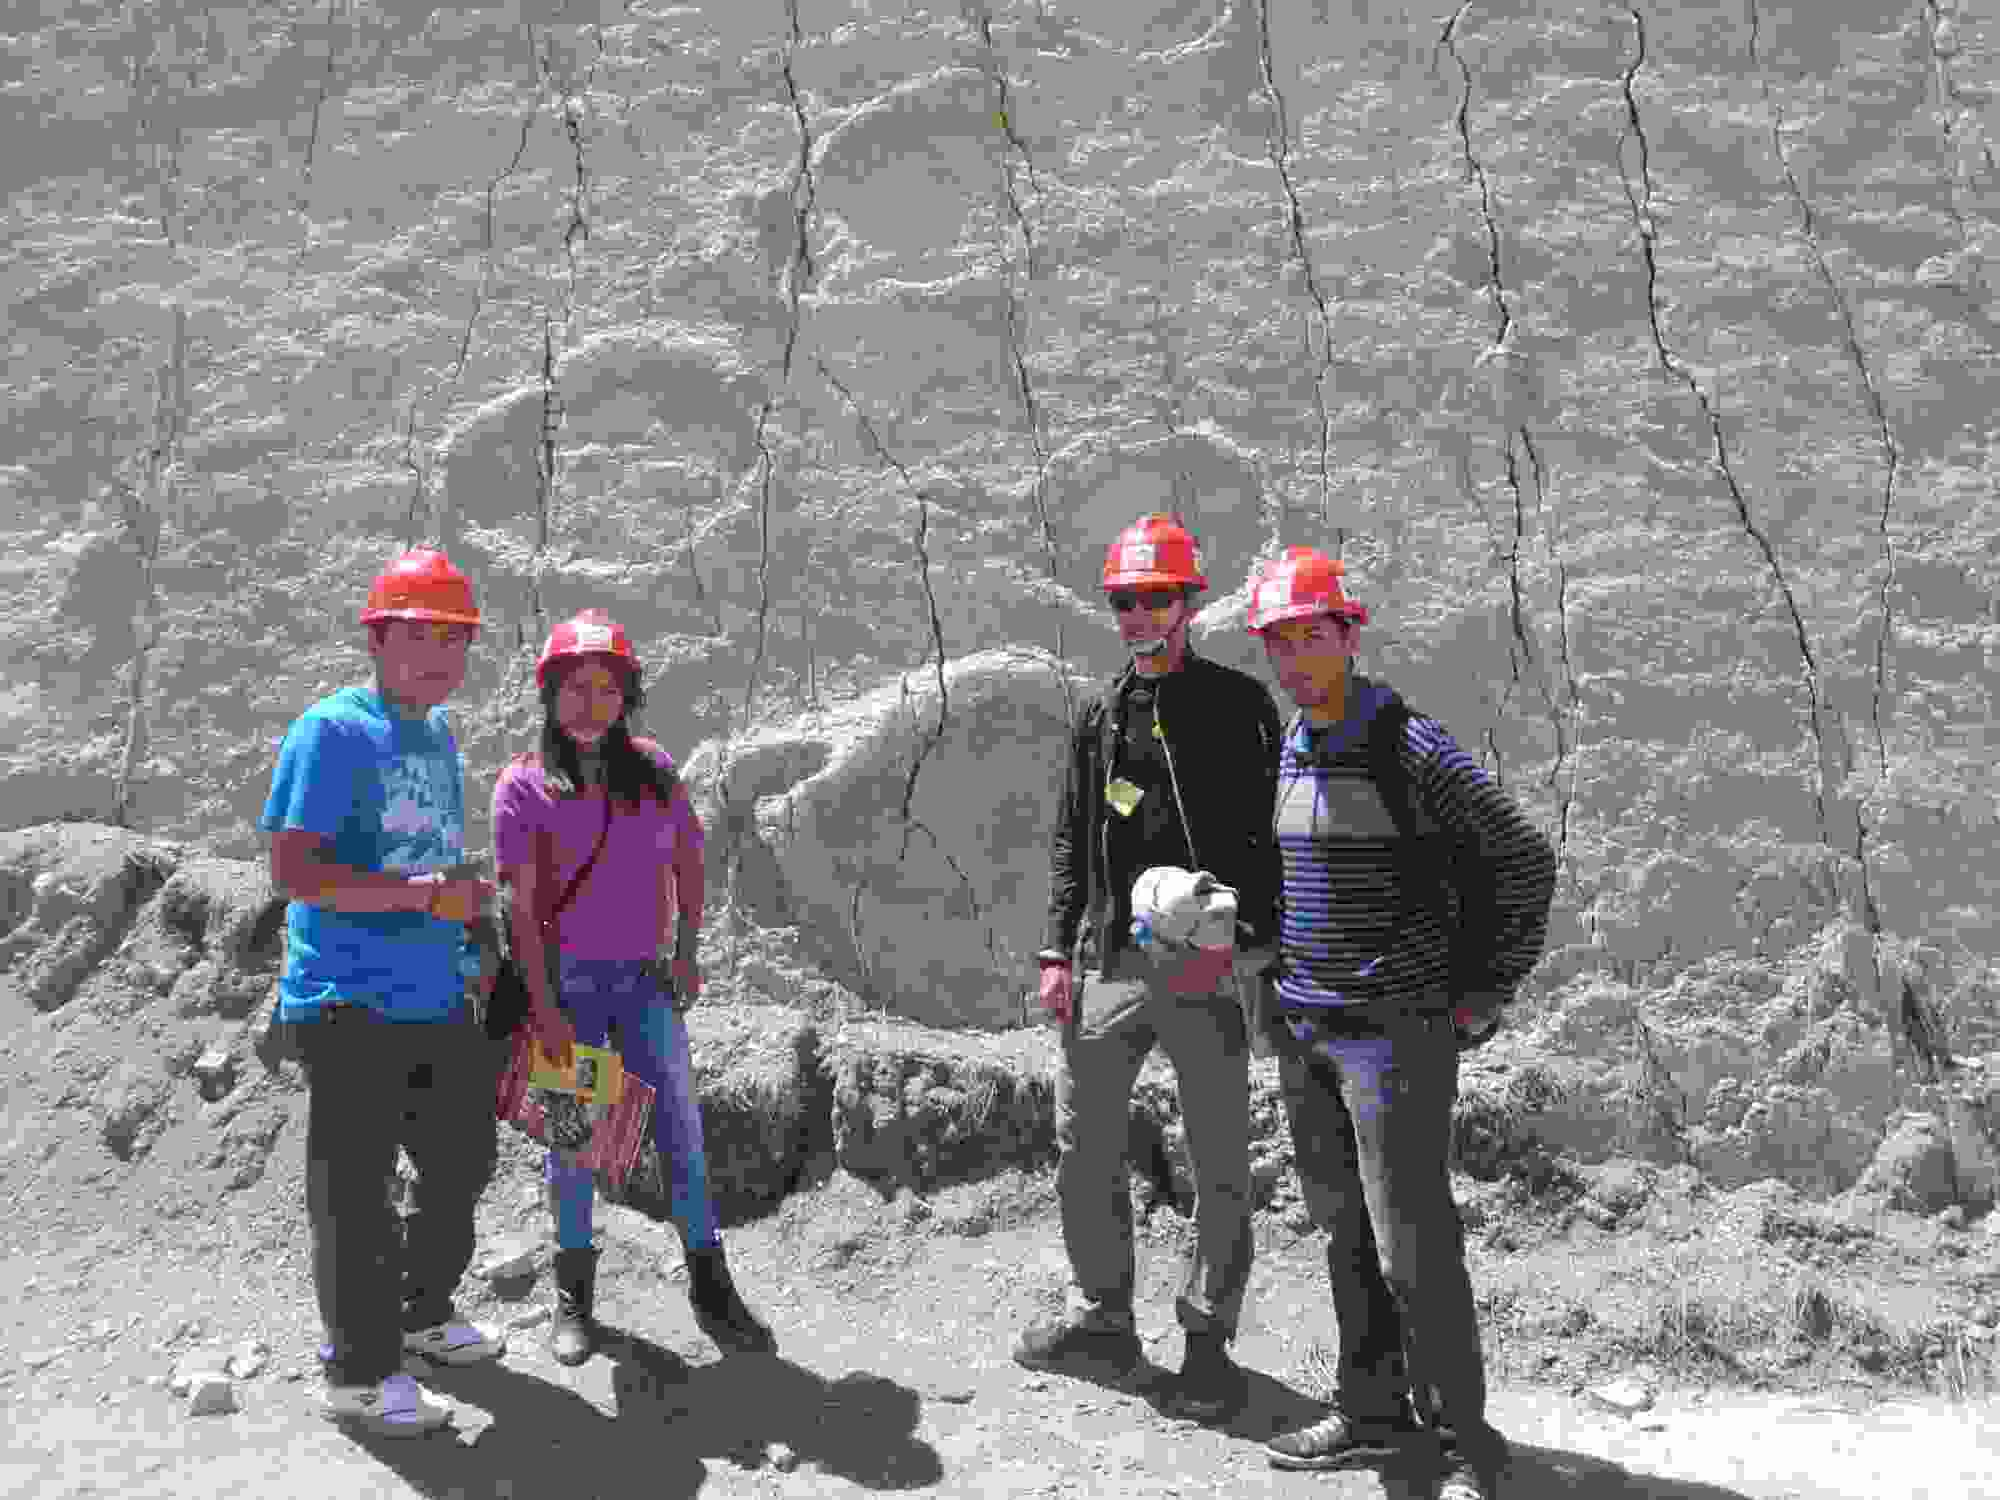
\includegraphics[width=\mywidth]{../wp-content/uploads/2015/04/wpid-wp-1429064728965.jpg} } 
 \newline

\newpage
 
